% This LaTeX document needs to be compiled with XeLaTeX.
\documentclass[
  10
]{article}
\usepackage[margin=2cm,includehead=true,includefoot=true,centering,]{geometry}
\usepackage{xcolor}
\usepackage{ucharclasses}
\usepackage{hyperref}
\usepackage{amsmath,amssymb}
\usepackage{amsfonts}
\usepackage[version=4]{mhchem}
\usepackage{stmaryrd}
\usepackage{bbold}
\usepackage{polyglossia}
\usepackage{fontspec}
\usepackage{ctex}
\usepackage[export]{adjustbox}
\usepackage{tabularx}
\usepackage{booktabs}

\usepackage{setspace}
\setstretch{1.2}

\makeatletter
\@ifundefined{KOMAClassName}{% if non-KOMA class
  \IfFileExists{parskip.sty}{%
    \usepackage{parskip}
  }{% else
    \setlength{\parindent}{0pt}
    \setlength{\parskip}{6pt plus 2pt minus 1pt}}
}{% if KOMA class
  \KOMAoptions{parskip=half}}
\makeatother
\usepackage{color}
\usepackage{fancyvrb}
\newcommand{\VerbBar}{|}
\newcommand{\VERB}{\Verb[commandchars=\\\{\}]}
\DefineVerbatimEnvironment{Highlighting}{Verbatim}{commandchars=\\\{\}}
% Add ',fontsize=\small' for more characters per line
\newenvironment{Shaded}{}{}
\newcommand{\AlertTok}[1]{\textcolor[rgb]{1.00,0.00,0.00}{\textbf{#1}}}
\newcommand{\AnnotationTok}[1]{\textcolor[rgb]{0.38,0.63,0.69}{\textbf{\textit{#1}}}}
\newcommand{\AttributeTok}[1]{\textcolor[rgb]{0.49,0.56,0.16}{#1}}
\newcommand{\BaseNTok}[1]{\textcolor[rgb]{0.25,0.63,0.44}{#1}}
\newcommand{\BuiltInTok}[1]{\textcolor[rgb]{0.00,0.50,0.00}{#1}}
\newcommand{\CharTok}[1]{\textcolor[rgb]{0.25,0.44,0.63}{#1}}
\newcommand{\CommentTok}[1]{\textcolor[rgb]{0.38,0.63,0.69}{\textit{#1}}}
\newcommand{\CommentVarTok}[1]{\textcolor[rgb]{0.38,0.63,0.69}{\textbf{\textit{#1}}}}
\newcommand{\ConstantTok}[1]{\textcolor[rgb]{0.53,0.00,0.00}{#1}}
\newcommand{\ControlFlowTok}[1]{\textcolor[rgb]{0.00,0.44,0.13}{\textbf{#1}}}
\newcommand{\DataTypeTok}[1]{\textcolor[rgb]{0.56,0.13,0.00}{#1}}
\newcommand{\DecValTok}[1]{\textcolor[rgb]{0.25,0.63,0.44}{#1}}
\newcommand{\DocumentationTok}[1]{\textcolor[rgb]{0.73,0.13,0.13}{\textit{#1}}}
\newcommand{\ErrorTok}[1]{\textcolor[rgb]{1.00,0.00,0.00}{\textbf{#1}}}
\newcommand{\ExtensionTok}[1]{#1}
\newcommand{\FloatTok}[1]{\textcolor[rgb]{0.25,0.63,0.44}{#1}}
\newcommand{\FunctionTok}[1]{\textcolor[rgb]{0.02,0.16,0.49}{#1}}
\newcommand{\ImportTok}[1]{\textcolor[rgb]{0.00,0.50,0.00}{\textbf{#1}}}
\newcommand{\InformationTok}[1]{\textcolor[rgb]{0.38,0.63,0.69}{\textbf{\textit{#1}}}}
\newcommand{\KeywordTok}[1]{\textcolor[rgb]{0.00,0.44,0.13}{\textbf{#1}}}
\newcommand{\NormalTok}[1]{#1}
\newcommand{\OperatorTok}[1]{\textcolor[rgb]{0.40,0.40,0.40}{#1}}
\newcommand{\OtherTok}[1]{\textcolor[rgb]{0.00,0.44,0.13}{#1}}
\newcommand{\PreprocessorTok}[1]{\textcolor[rgb]{0.74,0.48,0.00}{#1}}
\newcommand{\RegionMarkerTok}[1]{#1}
\newcommand{\SpecialCharTok}[1]{\textcolor[rgb]{0.25,0.44,0.63}{#1}}
\newcommand{\SpecialStringTok}[1]{\textcolor[rgb]{0.73,0.40,0.53}{#1}}
\newcommand{\StringTok}[1]{\textcolor[rgb]{0.25,0.44,0.63}{#1}}
\newcommand{\VariableTok}[1]{\textcolor[rgb]{0.10,0.09,0.49}{#1}}
\newcommand{\VerbatimStringTok}[1]{\textcolor[rgb]{0.25,0.44,0.63}{#1}}
\newcommand{\WarningTok}[1]{\textcolor[rgb]{0.38,0.63,0.69}{\textbf{\textit{#1}}}}
\usepackage{longtable,booktabs,array}
\newcounter{none} % for unnumbered tables
\usepackage{multirow}
\usepackage{calc} % for calculating minipage widths
% Correct order of tables after \paragraph or \subparagraph
\usepackage{etoolbox}
\makeatletter
\patchcmd\longtable{\par}{\if@noskipsec\mbox{}\fi\par}{}{}
\makeatother
% Allow footnotes in longtable head/foot
\IfFileExists{footnotehyper.sty}{\usepackage{footnotehyper}}{\usepackage{footnote}}
\makesavenoteenv{longtable}
\usepackage{graphicx}
\makeatletter
\newsavebox\pandoc@box
\newcommand*\pandocbounded[1]{% scales image to fit in text height/width
  \sbox\pandoc@box{#1}%
  \Gscale@div\@tempa{\textheight}{\dimexpr\ht\pandoc@box+\dp\pandoc@box\relax}%
  \Gscale@div\@tempb{\linewidth}{\wd\pandoc@box}%
  \ifdim\@tempb\p@<\@tempa\p@\let\@tempa\@tempb\fi% select the smaller of both
  \ifdim\@tempa\p@<\p@\scalebox{\@tempa}{\usebox\pandoc@box}%
  \else\usebox{\pandoc@box}%
  \fi%
}
% Set default figure placement to htbp
\def\fps@figure{htbp}
\makeatother
\setlength{\emergencystretch}{3em} % prevent overfull lines
\providecommand{\tightlist}{%
  \setlength{\itemsep}{0pt}\setlength{\parskip}{0pt}}


\hypersetup{colorlinks=true, linkcolor=blue, filecolor=magenta, urlcolor=cyan,}
\urlstyle{same}

\usepackage{colortbl}
\definecolor{table-row-color}{HTML}{999999}
\definecolor{table-rule-color}{HTML}{999999}
%\arrayrulecolor{black!40}
\arrayrulecolor{table-rule-color}     % color of \toprule, \midrule, \bottomrule
\setlength{\aboverulesep}{0pt}
\setlength{\belowrulesep}{0pt}


\setotherlanguages{english}
\IfFontExistsTF{Source Han Serif CN}
{\newfontfamily\chinesefont{Source Han Serif CN}}
{\IfFontExistsTF{Noto Serif CJK SC}
  {\newfontfamily\chinesefont{Noto Serif CJK SC}}
  {\IfFontExistsTF{SimSun}
    {\newfontfamily\chinesefont{SimSun}}
    {\IfFontExistsTF{FangSong}
      {\newfontfamily\chinesefont{FangSong}}
      {\newfontfamily\chinesefont{Arial Unicode MS}}
}}}
\IfFontExistsTF{Times New Roman}
{\newfontfamily\englishfont{Times New Roman}}
{\IfFontExistsTF{Liberation Serif}
  {\newfontfamily\englishfont{Liberation Serif}}
  {\IfFontExistsTF{DejaVu Serif}
    {\newfontfamily\englishfont{DejaVu Serif}}
    {\newfontfamily\englishfont{Arial}}
}}


\author{}
\date{}

\begin{document}


\section{MusaCoder: Native GPU Kernel Generation with Full-Stack
Training on Moore Threads
GPUs}\label{musacoder-native-gpu-kernel-generation-with-full-stack-training-on-moore-threads-gpus}

Kun Cheng1, Songshuo Lu1, Sicong Liao1, Tankun Li1, Yafei Zhang1 Dong
Yang, Qiheng Lv, Hua Wang, Zhi Chen2, Yaohua Tang

Moore Threads AI tangyaohua28@gmail.com

\pandocbounded{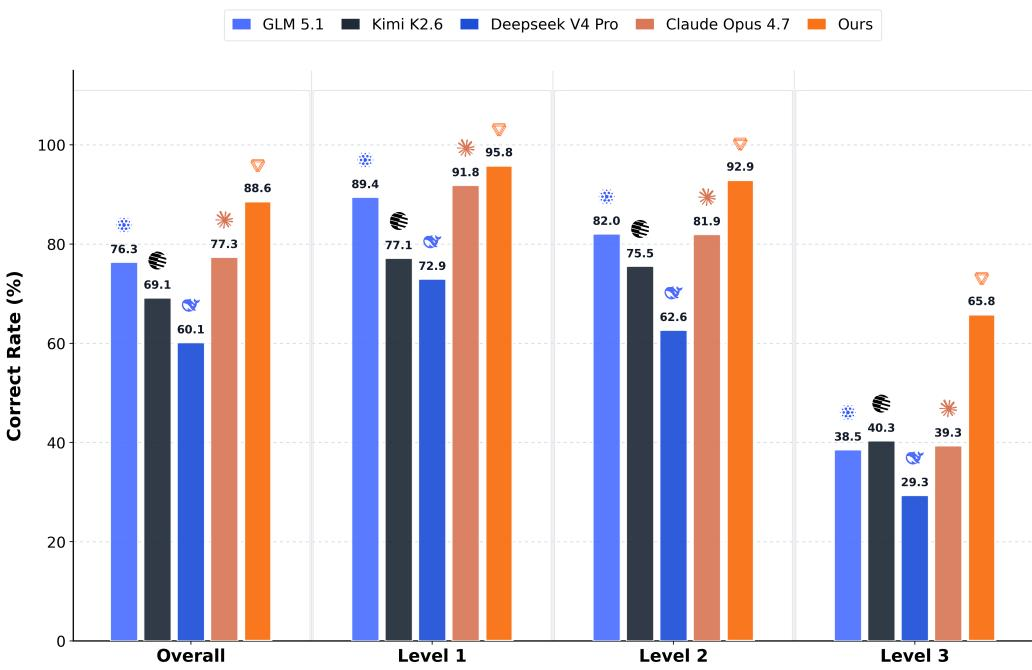
\includegraphics[keepaspectratio,alt={image}]{images/e381057e18bf06d53c5d4b48795a6f959d41e44b6310b10e6f11010766eac8f4.jpg}}

Figure 1: KernelBench performance comparison.

\subsection{ABSTRACT}\label{abstract}

Native GPU kernel generation turns high-level tensor programs into
executable, efficient low-level code. Existing Large Language Models
(LLMs) struggle with this task, while execution-based reinforcement
learning suffers from sparse rewards, reward hacking, and training
instability. We present MusaCoder, a full-stack training framework for
native GPU kernel generation on CUDA and MUSA backends. MusaCoder
combines progressive kernel-oriented data synthesis, diversitypreserving
rejection fine-tuning, and execution-feedback Reinforcement Learning
(RL) through MooreEval, a distributed verifier and reward environment.
To stabilize RL, MusaCoder introduces PrimeEcho for first-turn-anchored
multi-turn rewards, Buffered Dynamic Retry for recovering signals from
all-failed hard samples, and MirrorPop for off-policy sequence
filtering. Experiments on KernelBench and a MUSA-ported variant show
that MusaCoder outperforms strong open-source and proprietary baselines
in both correctness and empirical speedup, with the 9B model matching or
exceeding frontier closed-source models and the 27B model establishing a
new state of the art. These results demonstrate not only the
effectiveness of full-stack execution-feedback training for native
kernel generation, but also the capability of Moore Threads GPUs to
support the complete LLM post-training stack, providing a practical
foundation for large-model training and optimization on emerging
accelerators.

\subsection{1 INTRODUCTION}\label{introduction}

Modern neural networks increasingly rely on highly optimized GPU kernels
to fully utilize accelerator hardware. While vendor-specific libraries
(e.g., NVIDIA's cuBLAS and cuDNN) and static templates (e.g., CUTLASS)
deliver near-optimal performance for canonical operators, they struggle
to keep pace with the rapid proliferation of novel and long-tail
operator fusions in frontier AI models. Consequently, native GPU kernel
generation---translating high-level tensor computations directly into
optimized low-level device code---has become increasingly important.
Recently, Large Language Models (LLMs) have shown promising potential
for automating this process, offering a scalable alternative to
labor-intensive manual kernel engineering.

However, translating high-level PyTorch semantics into executable GPU
kernels with LLMs remains fundamentally challenging. Unlike
general-purpose code generation, synthesizing native kernels from
scratch suffers from extremely low initial success rates. Without
explicit domain grounding, off-the-shelf LLMs frequently struggle with
GPU execution semantics, mathematical derivations, and multi-dimensional
index mapping. Moreover, GPU kernels must satisfy strict correctness
constraints, requiring the generated code to be compilable, numerically
stable across edge cases, and compliant with hardware execution
semantics. As a result, even minor logical or mathematical errors can
lead to widespread compilation failures, illegal memory accesses, or
incorrect numerical outputs.

Recent years have witnessed the widespread adoption of reinforcement
learning (RL) with execution-based feedback in code generation. However,
extending these paradigms to GPU kernel generation introduces several
major challenges. First, reward sparsity: the high failure rate of
generated kernels often produces ``all-failed'' rollout groups, yielding
limited useful learning signal. Second, reward hacking: models tend to
exploit high-level API fallbacks (e.g., invoking torch.matmul or aten::*
routines) instead of generating fully native kernels. Third, off-policy
drift: the asynchronous and multi-turn nature of execution-based
rollouts amplifies gradient instability during training. These
challenges become even more pronounced in emerging non-CUDA accelerator
ecosystems, where large-scale training corpora and reliable verification
infrastructures remain limited.

To address these challenges, we present MusaCoder, an end-to-end
LLM-driven framework for native GPU kernel synthesis developed on Moore
Threads GPU clusters (Fig. 2). To deal with the extremely low initial
success rate of kernel generation and establish a strong policy
initialization, we design a comprehensive three-stage data synthesis
pipeline. Rather than relying on naive code translation, the pipeline
first expands task diversity and injects foundational CUDA/MUSA
knowledge to improve the model's understanding of GPU programming
semantics. It then introduces explicit tensor shape annotations and a
structured six-step reasoning format to guide the mapping from
high-level tensor operations to thread- and memory-level execution
semantics. Finally, the pipeline incorporates profiling analysis and
multi-turn interactive trajectories to reduce syntactic, logical, and
execution-level errors that would otherwise undermine the stability and
effectiveness of the overall synthesis pipeline.

Leveraging this progressive data pipeline, we first perform Multi-task
Supervised Fine-Tuning (SFT) to teach the model canonical kernel
generation patterns and error diagnosis behaviors. To further align the
model with execution correctness prior to RL, we subsequently apply
Diversity-Preserving Rejection Sampling Fine-Tuning (RFT). Conventional
RFT typically retains only the single fastest implementation, which can
lead to rapid entropy collapse and reduced exploration diversity. In
contrast, our approach employs an execution sandbox to filter
deterministic failures while deliberately preserving a heterogeneous set
of verified correct implementations. This stage substantially improves
absolute correctness while maintaining the behavioral diversity
necessary for effective downstream reinforcement learning

Building upon this diverse initialization, we formulate kernel synthesis
as a verifiable reinforcement learning problem. At the core of our RL
stage is MooreEval, a scalable distributed execution sandbox for
automated kernel evaluation. MooreEval enforces a strict
correctness-first verification hierarchy and incorporates anti-hacking
mechanisms to detect and penalize forbidden PyTorch fallbacks. Guided by
execution feedback from MooreEval, we employ a two-stage RL training
strategy consisting of a single-turn execution warmup followed by
iterative multi-turn feedback rollouts.

To improve the robustness and stability of execution-based RL, we
introduce three complementary stabilization mechanisms:

• PrimeEcho: A first-turn-anchored trajectory reward formulation that
incorporates multi-turn corrective feedback to improve exploration while
mitigating multi-turn reward hacking, without degrading zero-shot
generation quality.

• Buffered Dynamic Retry (BDR): A dynamic resampling strategy that
converts terminal all-failed groups into feedback-conditioned repair
tasks, recovering useful learning signals from difficult long-tail
samples and alleviating reward sparsity.

\pandocbounded{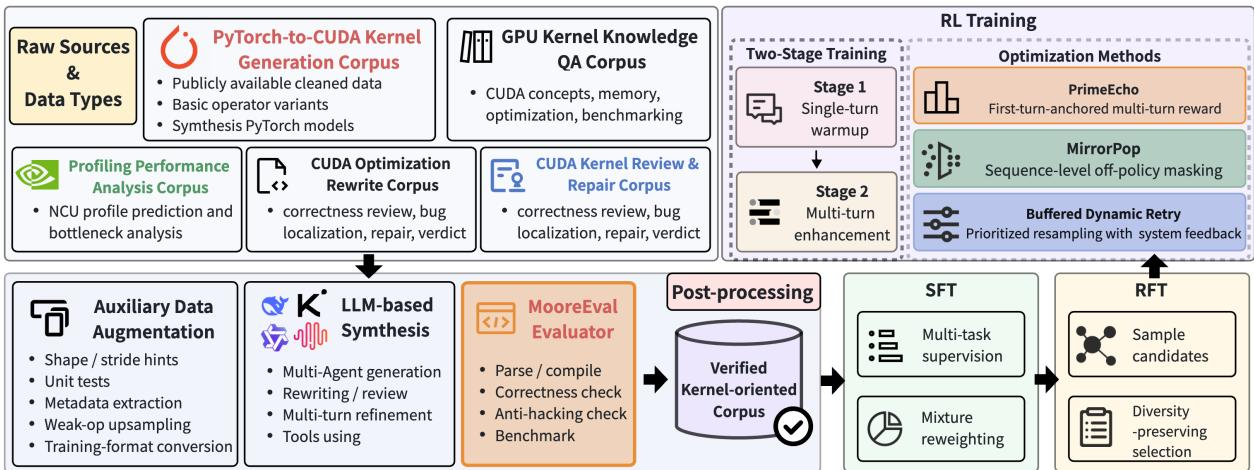
\includegraphics[keepaspectratio,alt={image}]{images/88f61ca6b2a473c6533f704bf2ca1da4384e2ca47bc2d6f9b7765b4363057200.jpg}}

Figure 2: Overview of the MusaCoder training pipeline. The pipeline
first constructs a kernel-oriented corpus from diverse raw sources,
including PyTorch-to-CUDA/MUSA generation data, GPU kernel knowledge QA,
profiling analysis, optimization rewrite, and kernel review/repair data.
The data are further augmented through shape/stride hints, unit tests,
metadata extraction, weak-operator upsampling, LLM-based synthesis, and
MooreEval-based verification. After post-processing, the verified corpus
is used for multi-task SFT and diversity-preserving RFT. Finally,
MusaCoder is optimized with a two-stage RL procedure, consisting of
single-turn warmup and multi-turn enhancement, together with three
stabilization techniques: PrimeEcho, MirrorPop, and Buffered Dynamic
Retry.

• MirrorPop: A sequence-level off-policy masking strategy that more
accurately estimates distributional drift magnitude, improving the
detection of severe off-policy samples and enabling more stable RL
training.

Empirical evaluations on the KernelBench suite and its MUSA-ported
variant show that MusaCoder significantly outperforms leading
proprietary and open-source models, including Claude Opus 4.7 and
DeepSeek-V4-Pro (Fig. 1). In particular, the 27B variant of MusaCoder
achieves state-of-the-art kernel correctness and runtime speedups. These
results demonstrate the effectiveness of our end-to-end alignment
pipeline in enabling hardware-aware GPU kernel generation, paving the
way toward fully automated kernel synthesis across platforms.

\subsection{2 RELATED WORK}\label{related-work}

LLM-driven GPU kernel generation has become an important research
direction in code synthesis. High-performance kernels are critical for
maximizing accelerator utilization in modern deep learning systems.
Unlike general-purpose program synthesis, GPU kernel generation imposes
strict execution requirements: generated kernels must compile
successfully, produce numerically correct outputs, avoid prohibited
high-level framework fallbacks, and deliver measurable runtime
improvements on real hardware. Consequently, recent research has
increasingly focused not only on code generation itself, but also on
execution-based evaluation, reward verification, and training models to
perform iterative error correction and repair.

\subsection{2.1 VENDOR LIBRARIES, COMPILERS, AND
DSLS}\label{vendor-libraries-compilers-and-dsls}

Existing approaches to high-performance GPU computing largely fall into
two paradigms. The first relies on highly optimized vendor libraries
such as NVIDIA's cuBLAS and cuDNN, as well as template-based frameworks
like CUT-LASS. While these libraries deliver excellent performance for
canonical operations such as GEMM and convolution, extending them to
support rapidly evolving model architectures, novel operators, and fused
computation patterns often requires substantial manual engineering
effort (Jaber and Jaber, 2026; Zhu et al., 2025). Moreover, modern deep
learning models introduce new computation patterns (e.g., SwiGLU and
Grouped-Query Attention) at a pace that frequently exceeds the update
cycles of vendor-maintained libraries and template frameworks.

To address this inflexibility, the systems community has heavily
invested in the second paradigm: bare-metal code generation (or native
kernel synthesis). Deep learning compilers and Domain-Specific Languages
(DSLs) were proposed to generate low-level code directly from
computational graphs (Chen et al., 2018; Zheng et al., 2020; Hsu et al.,

2024; Liu et al., 2023; Li et al., 2025a; Guo et al., 2026). Methods
like TVM (Chen et al., 2018) and Ansor (Zheng et al., 2020) map
optimization spaces into Intermediate Representations (IRs), using
search algorithms to find optimal implementations. Similarly, the Triton
ecosystem (Tillet et al., 2019) provides a higher abstraction for GPU
programming, with recent works exploring LLM integration within this DSL
space (Hsu et al., 2024; Li et al., 2025a). These pioneering systems
demonstrated that bypassing standard libraries is essential for fusing
operations and maximizing hardware utilization.

MusaCoder inherits this bare-metal synthesis philosophy. However,
instead of generating code that calls cuDNN/CUT-LASS or searching for
schedules in explicit IRs, MusaCoder is trained to write native
CUDA/MUSA kernels from scratch. By learning the mapping from PyTorch
reference programs to underlying hardware instructions, MusaCoder helps
developers support long-tail and novel operators without relying on
standard libraries, directly mastering lowlevel kernel design and
optimization.

\subsection{2.2 LLM-DRIVEN KERNEL GENERATION AND ITERATIVE
REFINEMENT}\label{llm-driven-kernel-generation-and-iterative-refinement}

Recent post-training methods for code and kernel generation have
expanded from supervised fine-tuning to verifierguided reinforcement
learning, multi-turn self-correction, and agent search (Madaan et al.,
2023; Shinn et al., 2023; Baronio et al., 2025; Li et al., 2025b; Dai et
al., 2026; Bai et al., 2026; Zhang et al., 2025; Brabec et al., 2025;
Dong et al., 2026; Yang et al., 2025). Works like Kevin (Baronio et al.,
2025) and CUDA-L1 (Li et al., 2025b) show that mastering kernel
generation requires learning from compiler, runtime, and performance
feedback via RL. Meanwhile, frozen-model agent systems (e.g., CUDA Agent
(Dai et al., 2026), CudaForge (Zhang et al., 2025), QiMeng-Kernel (Zhu
et al., 2025), and AutoKernel (Jaber and Jaber, 2026)) use LLMs at
inference time to interact with profilers and tools. More broadly,
software engineering frameworks like OpenHands and SWE-agent (Wang et
al., 2024; Yang et al., 2024), along with self-correction studies (Ding
et al., 2024; Ye et al., 2025; Wang et al., 2025), show the
effectiveness of using test-time computation to improve code quality.

While agent-based methods achieve strong performance by relying on
massive inference-time computation, MusaCoder internalizes these
capabilities directly into the model weights through an SFT →
single-turn RL → multiturn RL pipeline. By embedding compiler and
runtime feedback into the training loop, MusaCoder empowers much smaller
models (e.g., 9B parameters) to surpass the accuracy of state-of-the-art
closed-source models. This approach fundamentally eliminates the
reliance on extensive test-time search, drastically reducing deployment
and inference costs while retaining the model's ability to autonomously
fix errors and optimize code.

\subsection{2.3 EXECUTABLE EVALUATION AND REWARD
VERIFICATION}\label{executable-evaluation-and-reward-verification}

Benchmarking and verifier design are essential for execution-driven
generation. Frameworks like Kernel-Bench (Ouyang et al., 2025) and
KernelBenchX (Wang et al., 2026), along with other executable
evaluations (Baronio et al., 2025; Li et al., 2025b; Dai et al., 2026;
Bai et al., 2026; Brabec et al., 2025), require outputs to pass actual
compilation, random testing, and synchronized profiling, rather than
just measuring text similarity.

Furthermore, GPU kernel generation is prone to reward hacking, such as
calling forbidden PyTorch operators, using asynchronous execution to
bypass timers, or modifying benchmark settings. Therefore, recent
systems emphasize strict anti-cheating mechanisms (Wang et al., 2026; Li
et al., 2025b; Dai et al., 2026; Zhang et al., 2025; Zhu et al., 2025).
MusaCoder adopts this approach. Our verifier categorizes outputs into
compilation failures, runtime exceptions, correctness failures,
cheating/fallback behaviors, and valid performance metrics. This
structured feedback prevents evaluation loopholes and provides precise
debugging information for multi-turn RL.

\subsection{2.4 EMERGING ACCELERATOR ECOSYSTEMS AND MUSACODER'S
POSITIONING}\label{emerging-accelerator-ecosystems-and-musacoders-positioning}

While CUDA remains the dominant ecosystem, software stacks for emerging
alternative accelerators---such as Huawei's CANN (Huawei, 2026),
Cambricon's BANG (Cambricon, 2026), and Moore Threads' MUSA SDK (Moore
Threads, 2026)---are developing rapidly. A major systems challenge in
these heterogeneous ecosystems is the high manual engineering cost of
migrating and optimizing novel operators across different platforms. A
model that can generate native kernels from scratch can significantly
reduce this cross-platform development cost and mitigate vendor lock-in.
MusaCoder addresses this problem by training CUDA and MUSA kernel
generators within a unified full-stack pipeline on Moore Threads GPUs,
showing that emerging accelerators can support closed-loop LLM
post-training for executable code generation.

\pandocbounded{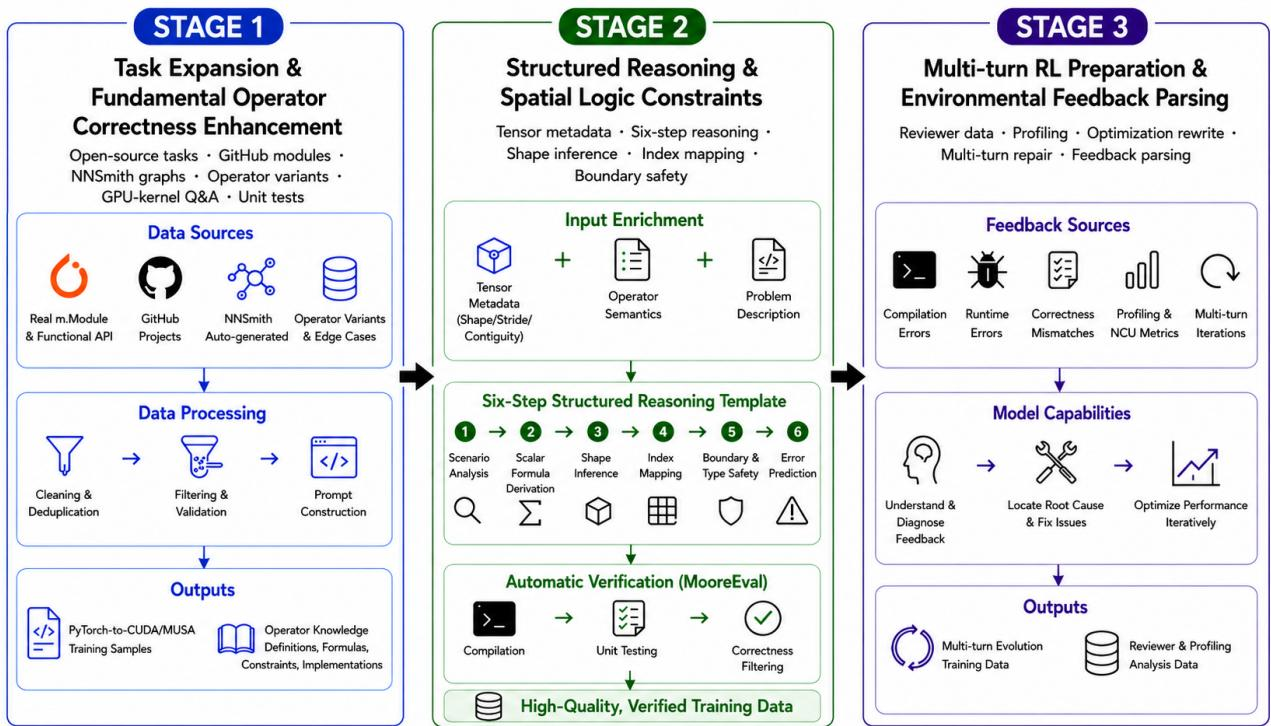
\includegraphics[keepaspectratio,alt={image}]{images/9a8b249547cc727ba7db49389ca8ef62236da9b18fd01fff966f530faf0be717.jpg}}

Figure 3: Three-stage evolution of the SFT data construction pipeline.
Stage 1 expands the PyTorch-to-CUDA/MUSA workload distribution and
aligns baseline operator correctness through real PyTorch modules,
GitHub projects, NNSmith-generated graphs, operator variants, cleaning,
filtering, and prompt construction. Stage 2 injects tensor metadata and
enforces a six-step structured reasoning template to strengthen shape
inference, index mapping, boundary handling, and semantic correctness,
followed by MooreEval-based automatic verification. Stage 3 introduces
execution-feedback understanding through compilation errors, runtime
failures, correctness mismatches, profiling signals, and multi-turn
iterations, producing data for feedback-driven repair, reviewer
training, and performance optimization.

\subsection{3 DATA SYNTHESIS PIPELINE}\label{data-synthesis-pipeline}

Existing PyTorch-to-CUDA datasets are useful for KernelBench-style
warmup, but they are not sufficient for fullstack post-training. They
provide limited coverage of long-tail operators, often lack reusable
verification assets, and may rely on vendor-library implementations
rather than native kernels. MusaCoder therefore constructs SFT data as a
staged capability-building process (Fig. 3).

• Stage 1: Task Expansion and Fundamental Operator Correctness
Enhancement. We enlarge PyTorchto-CUDA/MUSA task coverage with
open-source tasks, GitHub modules, NNSmith-generated graphs, targeted
basic-operator variants, GPU-kernel Q\&A data, and automatically
generated unit tests.

• Stage 2: Structured Reasoning and Spatial Logic Constraints. We add
explicit tensor metadata and a sixstep reasoning template to reduce
common failures in shape inference, scalar formulas, indexing, boundary
handling, and fallback avoidance.

• Stage 3: Multi-turn RL Preparation and Environmental Feedback Parsing.
We synthesize reviewer, profiling, optimization-rewrite, and multi-turn
repair data so that the model can interpret compiler/runtime errors,
correctness mismatches, and performance feedback before RL

Through the aforementioned three-stage pipeline, MusaCoder's SFT data
evolves from simple PyTorch-to-CUDA/MUSA translation pairs into a rich
training corpus that integrates operator knowledge, structured
reasoning, automated verification, and execution-feedback parsing. This
pipeline not only improves the model's execution correctness in
generating native CUDA/MUSA kernels, but also strengthens its ability to
interpret compiler errors, runtime feedback, and performance
bottlenecks. As a result, it provides a strong and stable initialization
for subsequent RFT and RL training while preserving sufficient
behavioral diversity for effective exploration.

\subsection{3.1 TASK EXPANSION AND FUNDAMENTAL OPERATOR CORRECTNESS
ENHANCEMENT}\label{task-expansion-and-fundamental-operator-correctness-enhancement}

\subsection{3.1.1 PYTORCH-TO-CUDA/MUSA WORKLOAD
EXPANSION}\label{pytorch-to-cudamusa-workload-expansion}

This stage first expands the scale and distributional coverage of
PyTorch-to-CUDA/MUSA generation tasks. Rather than relying on a narrow
set of manually written operators, we construct reference workloads from
three complementary sources: existing open-source PyTorch modules and
kernel generation tasks (Dai et al., 2026; Gope et al., 2024),
real-world PyTorch modules and functional API calls from GitHub
repositories, and valid PyTorch computation graphs automatically
synthesized by NNSmith (Liu et al., 2023). Open-source data provides
representative kernel-generation scenarios, GitHub data introduces
realistic module structures and operator compositions, and NNSmith
systematically supplements workload regions that are insufficiently
covered by manually collected or real-world code.

For the GitHub data, we perform rigorous cleaning, deduplication, and
filtering. We eliminate samples that depend on external states, contain
unstable control flows, or are difficult to verify, retaining only
reference programs that can be converted into executable
PyTorch-to-CUDA/MUSA generation tasks.

We employ NNSmith to synthesize executable computation graphs under
strict operator, shape, and dtype constraints. The operator pool covers
activation functions, basic mathematical operations, logical operations,
shape manipulations, pooling, reductions, normalization layers,
convolution variants, interpolation, padding, type casting, and matrix
operations. We further extend this pool to include 1D/3D operators,
transposed convolutions, PixelShuffle, Adaptive Pooling, Dropout, Bmm,
Addmm, and normalization variants, ultimately covering approximately 162
empirically tested operators. During generation, we specify operator
subsets via mgen.include, control graph size via mgen.max nodes, and
direct the generation of 1D, 2D, or 3D workloads via mgen.rank choices.
This facilitates the construction of diverse graph archetypes, such as
CNN-like, 3D convolutional, 1D sequential, reductionheavy, and
shape-sensitive computation graphs. All generated computation graphs are
validated via the TorchScript backend and filtered based on
executability, input-output stability, graph scale, and task
adaptability before being converted into kernel generation prompts.

\subsection{3.1.2 BASIC OPERATOR VARIANT
AUGMENTATION}\label{basic-operator-variant-augmentation}

Workload expansion alone does not resolve the model's weaknesses on
fundamental operator semantics. Early experiments show that the model's
accuracy is close to zero on several basic operator families, especially
convolution variants. Under diverse parameter configurations, including
varying strides, paddings, dilations, groups, kernel sizes, input ranks,
1D/2D/3D convolutions, and transposed convolutions, the model frequently
fails in semantic interpretation, shape inference, boundary handling,
and index mapping. Because these operators serve as essential building
blocks for complex models and fused kernels, unstable correctness at
this level would flood the subsequent RL stage with invalid samples and
substantially weaken executable learning signals.

To address this issue, we construct large-scale variant data for
fundamental operators. The dataset spans diverse dtypes, shapes,
broadcast patterns, reduction dimensions, contiguous and non-contiguous
layouts, and extreme input scenarios. Guided by failure distributions
observed in preliminary validation, we upsample vulnerable operator
families, including nn.Conv2d, transposed convolutions, 3D convolutions,
reductions, normalizations, softmax, broadcasting, and complex indexing.
This targeted augmentation is designed not merely to increase data
volume, but to expose the model to the parameter regimes and boundary
cases where basic operator generation most often breaks down.

The construction pipeline consists of ``Data Pre-processing → Two-Stage
LLM Generation → Compilation and Correctness Filtering.'' In the
pre-processing stage, we aggregate real-world PyTorch code snippets and
low-level operator APIs. We employ Small Language Models (SLMs) for
semantic cleansing to eliminate state-control APIs (e.g., torch.set
device()), retaining exclusively pure computational operators as
generation seeds. In the first stage of LLM generation, rather than
directly outputting CUDA code, we prompt the LLM to design diverse
implementation pathways for a given operator, including naive baselines,
single-feature optimizations, algorithmic or input-specialized
implementations, and composite optimized variants. Each pathway must
explicitly define the thread mapping, memory hierarchy transitions,
synchronization primitives, and resource bottleneck trade-offs, thereby
forming a structured mechanism description. In the second stage, the LLM
generates concrete CUDA kernels based on these mechanisms and target
scenarios. Compared with generating code directly from operator
descriptions, this ``plan-then-implement'' paradigm reduces monotonic
template outputs and improves implementation diversity. Finally, we
couple candidate implementations with automatically generated unit tests
for compilation, execution, and correctness verification, filtering out
samples that fail to compile, trigger runtime errors, exhibit numerical
inconsistencies, or display suspicious speculative behaviors.

Overall, this stage establishes the data foundation for
PyTorch-to-CUDA/MUSA tasks through two complementary interventions.
Workload expansion broadens the distribution of reference programs and
operator compositions, while basic operator variant augmentation
directly targets the model's most severe fundamental correctness
failures, especially convolution, reduction, normalization,
broadcasting, and complex indexing. Together, they provide a more stable
correctness baseline for the subsequent structured reasoning, multi-turn
feedback, and RL phases.

\subsection{3.1.3 GPU KERNEL KNOWLEDGE Q\&A
DATA}\label{gpu-kernel-knowledge-qa-data}

Beyond direct PyTorch-to-CUDA/MUSA generation data, we construct a GPU
Kernel Knowledge Question-and-Answer (Q\&A) dataset to supplement the
model's foundational knowledge encompassing mathematical principles,
CUDA programming models, GPU architectures, PyTorch tensor semantics,
memory hierarchies, performance optimization strategies, numerical
stability, and benchmarking methodologies. We observe that many errors
in kernel generation do not merely stem from the code implementation
itself, but rather originate from an inadequate comprehension of
underlying concepts. Examples include erroneous thread indexing,
neglected boundary checks, misjudged tensor layouts, mishandled
reduction precision, or a lack of understanding regarding the impact of
asynchronous CUDA execution on latency measurement. Therefore, this
dataset aims to equip the model with more robust knowledge priors for
kernel generation.

The questions in this dataset are primarily sourced from two pipelines.
The first pipeline extracts data from opensource CUDA tutorials, GPU
programming documentation (NVIDIA, 2026a), kernel optimization examples,
and common CUDA bug/FAQ repositories via rule matching, keyword
extraction, and manual cleansing, predominantly covering general
concepts and common optimization principles. The second pipeline
synthesizes questions based on KernelBench task patterns and the model's
failure cases from the previous kernel generation stage, serving to
precisely bridge the model's exposed vulnerabilities. Specifically, we
perform targeted augmentation for operator types that exhibit low
accuracy or suboptimal performance during direct kernel generation, such
as convolution, reduction, normalization, softmax, broadcasting, and
complex shape indexing.

Distinct from direct kernel generation data, the knowledge Q\&A data
does not require the model to output complete CUDA implementations.
Instead, it trains the model to conduct deep causal reasoning:
elucidating why a particular implementation is efficient, how underlying
physical constraints restrict code topologies, and identifying the root
causes of specific runtime errors. The questions encompass mathematical
definitions, basic CUDA implementations and memory access optimizations,
high-performance tuning, Tensor Core utilization and hardware
adaptation, common bug debugging and bottleneck analysis, advanced
applications, and future architectural evolutions. This data serves as a
knowledge enhancement signal during SFT, forming a complement to the
code generation data: the generation data teaches the model how to write
kernels, whereas the knowledge Q\&A data helps the model comprehend the
underlying rationale for correctness and performance behind specific
implementation choices.

\subsection{3.1.4 AUTOMATED UNIT TEST GENERATION AND
VERIFICATION}\label{automated-unit-test-generation-and-verification}

To guarantee the executability and correctness of the synthesized data,
we construct an automated unit test generation and verification pipeline
for PyTorch-to-CUDA/MUSA tasks. For a given PyTorch reference program,
the code alone is insufficient to determine the correctness of the
generated kernel; it necessitates test cases encompassing diverse input
shapes, data types, value ranges, and edge cases. Therefore, we leverage
Large Language Models (LLMs) to generate candidate test cases based on
PyTorch code semantics and interface signatures, and execute them within
a native PyTorch environment to obtain reference outputs (ground truth)
for subsequent sample filtering and MooreEval evaluation.

Specifically, test case generation primarily covers four dimensions of
variation. First is shape coverage, including regular dimensions,
unaligned dimensions, highly imbalanced dimensions, and shape
combinations that trigger broadcasting. Second is dtype coverage,
encompassing FP32, FP16, BF16, and common integer inputs. Third is value
range coverage, which includes standard random distributions, mixed
positive and negative values, zero-inclusive inputs, and extreme
maximum/minimum values that may trigger overflow, underflow, or
numerically unstable paths. Finally, edge case coverage involves
scenarios such as empty tensors, all-zero/all-one inputs, non-contiguous
tensors, and special dimensional configurations.

The generated candidate test cases are initially executed in the native
PyTorch environment. We filter out test samples that exhibit syntax
errors, invalid parameter combinations, runtime exceptions,
out-of-memory (OOM) errors, or unstable outputs, retaining only those
cases that execute stably and yield deterministic reference outputs. The
retained test suite is subsequently utilized in two scenarios: first,
during the SFT data construction phase for compiling and
correctness-filtering candidate CUDA/MUSA implementations; second,
within the subsequent MooreEval framework for random-input correctness
checks and performance profiling of model-generated results. Through
this pipeline, we mitigate the influx of erroneous implementations into
the training data while providing a unified, reusable evaluation
foundation for the ensuing RFT/RL phases.

In summary, this stage establishes the foundational data substrate
across three dimensions: tasks, knowledge, and verification. The
PyTorch-to-CUDA/MUSA data broadens the task distributions exposed to the
model; the knowledge Q\&A data supplements the underlying CUDA and
PyTorch semantic priors; and the automated unit tests provide a unified
standard for data filtering and subsequent execution-based evaluations.
The objective of this stage is not to directly pursue optimal
performance, but rather to prioritize enhancing the executability,
semantic correctness, and fundamental robustness of the generated
results.

\subsection{3.2 STRUCTURED REASONING AND SPATIAL LOGIC
CONSTRAINTS}\label{structured-reasoning-and-spatial-logic-constraints}

\subsection{3.2.1 STANDARDIZED DATA STRUCTURE FOR SIX-STEP
REASONING}\label{standardized-data-structure-for-six-step-reasoning}

During direct CUDA kernel generation, models frequently bypass
intermediate reasoning steps, leaping straight from PyTorch code to
low-level implementations. This often results in logical disjoints
across operator semantic comprehension, shape inference, index mapping,
boundary handling, and numerical stability. To mitigate these logical
disjoints, we introduce a six-step reasoning format into the SFT data,
decomposing the PyTorch-to-CUDA/MUSA translation process into an ordered
sequence of intermediate reasoning steps. The objective of this format
is not to induce redundant explanations, but to compel the model to
execute a structured derivation---from high-level operator semantics to
thread-level memory accesses---prior to code generation.

The six-step reasoning structure is defined as follows:

Step 1: Holistic Analysis and Operator Deconstruction Analyze the
primary computational paradigm of the Py-Torch code (e.g., element-wise
operations, reductions, matrix multiplications, or spatial
transformations), and explicitly list the involved inputs, outputs, and
critical parameters such as weight, bias, stride, and padding. This
phase establishes the mapping between PyTorch APIs and low-level kernel
inputs, mitigating issues related to omitted parameters or
misinterpreted operator semantics.

Step 2: Scalar Mathematical Formula Derivation Deconstruct tensor-level
operations in PyTorch into the scalar computations required for a single
output element or a single thread. For example, for normalization
operators, the calculation formulas for mean, variance, normalization,
and affine transformations must be explicitly defined. This phase
facilitates the paradigm shift from tensor-level expressions to
thread-level computational logic.

Step 3: Shape and Dimensionality Calculus Deduce the shape transitions
across input, intermediate, and output tensors, clarifying the
dimensional impact of operations such as broadcasting, reshape,
transpose, slice, pooling, convolution, and reduction. For reduction
operations, the reduction domain must also be explicitly determined.
This phase provides the geometric basis for subsequent determinations of
total thread counts, grid/block configurations, and output memory
layouts.

Step 4: Indexing Relations and Memory Mapping Establish the
bi-directional mapping between 1D global thread indices and
multi-dimensional logical coordinates, and compute the corresponding
linear memory offsets based on the tensor layout. For non-contiguous
tensors, explicit address calculations incorporating strides are
mandated. This phase is primarily designed to minimize erroneous
indexing, out-of-bounds memory accesses, and incorrect dimensional
unrolling.

Step 5: Boundary Handling and Type Safety Analyze edge cases requiring
explicit handling within the kernel, such as out-of-bounds protection
for trailing threads, padding regions, division-by-zero risks,
low-precision accumulation errors, integer/floating-point type casting,
and anomalous shapes. This phase guides the model to inject necessary
defensive logic, thereby enhancing code robustness across diverse input
conditions.

Step 6: Error Pre-analysis and Negative Constraints Summarize potential
pitfalls in the current task based on historical failure modes---such as
hardcoding dimensions, ignoring strides, omitting biases, mishandling
broadcasting, inappropriately assuming contiguous memory layouts, or
invoking disallowed PyTorch fallbacks. Serving as a pre-generation
self-diagnostic step, this phase prevents the model from reiterating
highfrequency errors.

Through this standardized format, we decompose end-to-end code
generation into a six-dimensional intermediate reasoning process
encompassing semantics, mathematics, shape, indexing, boundaries, and
error pre-analysis. During the SFT phase, this format serves as
high-quality reasoning traces incorporated into the training corpus,
enabling the model to internalize a more stable and deterministic kernel
generation workflow. In subsequent inference or multiturn rectification
scenarios, the model can leverage this structured intermediate
representation for self-diagnosis and precise bug localization.

\subsection{3.2.2 EXPLICIT TENSOR SHAPE
ANNOTATION}\label{explicit-tensor-shape-annotation}

We observe that models frequently stumble in PyTorch-to-CUDA/MUSA
generation during shape-sensitive operations, such as view/reshape,
transpose, broadcasting, slicing, pooling, convolution, and reduction.
Once an error occurs in deducing the output shape or the layout of an
intermediate tensor, the subsequent determinations of grid sizes, thread
indices, memory offsets, and output write-back locations inherently
cascade into failure. To mitigate such shape reasoning errors, we
introduce an explicit shape annotation strategy during the construction
of training samples: subsequent to the original PyTorch reference code
but prior to the model's generation of the CUDA/MUSA kernel, we append a
structured {[}Tensor Shape Information{]} block. This block explicitly
enumerates the shapes, strides, and contiguity flags of critical inputs,
intermediate nodes, and output tensors. Consequently, the model is
directly exposed to explicit tensor layout constraints prior to kernel
generation, rather than relying exclusively on implicit reasoning
derived from the PyTorch code.

Specifically, we automatically extract tensor metadata from the PyTorch
computation graph via predefined graph anal ysis scripts. PyTorch's
dynamic graph mechanism, torch.fx graph capture, and shape propagation
provide the foundational utilities for this precise metadata extraction
(Paszke et al., 2019; Reed et al., 2022). For tasks with static input
dimensions, we employ a static analysis pipeline based on torch.fx: we
first trace the computation graph via torch.fx.symbolic trace, and
subsequently execute ShapeProp with dummy inputs to extract the concrete
shape, stride, and is contiguous attributes from the tensor meta of each
critical node. For tasks featuring dynamic input dimensions, we adopt a
symbolic pipeline based on torch.export. We represent dynamic dimensions
via torch.export.Dim and extract symbolic shape and stride expressions
from the exported ExportedProgram. For instance, given a slice operation
on an input of shape {[}B, L{]}, the system can record the output shape
as {[}B, L − 1{]} while preserving the stride semantics of that sliced
view.

In the final prompt, this annotation is inserted immediately following
the PyTorch reference in a format akin to the following:

\begin{Shaded}
\begin{Highlighting}[]
\NormalTok{Shape{-}enhanced prompt block}
\NormalTok{[Tensor Shape Information]}
\NormalTok{{-} input x: shape=[B, L], stride=[L, 1], contiguous=True}
\NormalTok{{-} narrow/slice node: shape=[B, L{-}1], stride=[L, 1], contiguous=False}
\NormalTok{{-} cumsum node: shape=[B, L{-}1], stride=[L{-}1, 1], contiguous=True}
\NormalTok{{-} output: shape=[B, L], stride=[L, 1], contiguous=True}
\NormalTok{[Kernel Generation Hint]}
\NormalTok{Use the listed shapes and strides when deriving thread mapping and memory offsets.}
\NormalTok{Do not assume an intermediate tensor is contiguous unless marked contiguous=True. }
\end{Highlighting}
\end{Shaded}

This specific placement integrates the shape annotation intrinsically
into the generation task itself, rather than treating it as a disjoint
offline analysis log. For non-contiguous views, the prompt explicitly
provides the strides and instructs the model to employ stride-based
address calculations, averting the default assumption of contiguous
memory layouts. For operations such as reshape, transpose, broadcast,
and reduction, the annotation retains the input-output shape transitions
of critical nodes, guiding the model in determining total thread counts,
output coordinate unrolling schemes, and write-back indices.

This strategy is primarily utilized during SFT data construction, though
it can also serve as explicit prompt augmentation during inference.
During training, it provides the model with explicit tensor layout
supervision, training it to align shapes, strides, and output layouts
prior to writing the kernel. During inference, it reduces the model's
misjudgments regarding complex shapes and non-contiguous memory layouts.
Because we have thus far only conducted manual inspections on a limited
subset of shape mismatch cases and their rectified outcomes, without yet
formalizing systematic ablation studies, we do not present this as a
standalone empirical claim in this paper. Instead, we provide a
representative case study in the Appendix C to demonstrate how explicit
shape annotation facilitates the correction of indexing logic.

\subsection{3.3 MULTI-TURN RL PREPARATION AND ENVIRONMENTAL FEEDBACK
PARSING}\label{multi-turn-rl-preparation-and-environmental-feedback-parsing}

\subsection{3.3.1 MULTI-TURN INTERACTIVE TRAJECTORY SYNTHESIS AND
CONTEXT
PRE-ADAPTATION}\label{multi-turn-interactive-trajectory-synthesis-and-context-pre-adaptation}

During single-turn CUDA kernel generation, models frequently struggle to
simultaneously satisfy compilation, numerical correctness, and
performance constraints. Compared to static PyTorch-to-CUDA/MUSA
samples, the environmental feedback returned by the evaluation
sandbox---such as textual compilation/runtime errors and quantitative
performance metrics---provides explicit rectification signals. To lay
the empirical foundation for subsequent multiturn Reinforcement Learning
(RL), we synthesize multi-turn iterative interaction trajectories during
this stage. This not only trains the model to parse environmental
feedback and localize functional or micro-architectural bugs, but
crucially allows it to pre-adapt to the multi-turn conversational
context and dependency structures, thereby executing targeted
self-correction.

Specifically, we adopt a ``5 + 3'' multi-turn interactive rollout
mechanism. For each task, the model initially generates a candidate
kernel, which is submitted to the MooreEval sandbox for verification. If
the candidate implementation fails compilation or correctness checks,
the subsequent prompt injects the error logs, numerical discrepancies,
or failure rationales from the preceding turn, guiding the model to
execute bug rectification. Conversely, if the candidate implementation
is functionally correct, subsequent turns pivot towards performance
optimization, prompting the model to refine memory access patterns,
thread partitioning, synchronization strategies, or kernel fusion based
on the current implementation. By default, a maximum of 5 iterative
turns is permitted; to enhance the coverage of hard tasks, an additional
allowance of up to 3 rectification attempts is granted.

Regarding trajectory retention, we mandate that the final-turn output
must pass correctness verification, and we prioritize retaining
trajectories that exhibit significant performance gains relative to
their historical correct versions. Specifically, if a trajectory
contains multiple correct implementations, we designate the first
correct version as the performance baseline and require the final
version to achieve a speedup of at least 1.2×. This criterion prevents
the training set from being inundated with protracted rectification
trajectories that lack optimization dividends. Concurrently, failure
samples induced by environmental anomalies, timeouts, or
non-model-related infrastructure issues are meticulously purged during
the filtering phase to prevent the injection of noisy feedback.

During training, the historical turns within the multi-turn trajectories
function primarily as contextual inputs, supplying error diagnostics and
evolutionary topologies; the specific loss masking strategies will be
detailed comprehensively in the SFT training section. Fundamentally,
this data compels the model to transcend the mere imitation of static
code snapshots, enabling it to master dynamic parsing and refactoring
driven by environmental feedback. This paradigm establishes an optimal
policy initialization and context adaptation for the subsequent
closed-loop, multi-turn RL training phase.

\subsection{3.3.2 CUDA KERNEL REVIEWER}\label{cuda-kernel-reviewer}

To elevate the model's diagnostic proficiency regarding the correctness
and performance bottlenecks of CUDA kernels, we construct specialized
CUDA Kernel Reviewer data. Taking a PyTorch reference code and a
candidate CUDA kernel as inputs, this data tasks the model with
verifying whether the candidate implementation aligns with the PyTorch
semantics. If an error is detected, the model must provide a root-cause
analysis alongside the rectified code; if the candidate kernel is
functionally correct, the model must further profile its potential
performance bottlenecks. In contrast to direct kernel generation data,
the Reviewer data does not primarily train the model to author kernels
de novo. Instead, it compels the model to comprehend the underlying
causality---why a kernel succeeds or fails, and how it can be
systematically rectified or optimized.

Each Reviewer sample comprises two input components: the PyTorch
reference code, which delineates the target computational semantics, and
the candidate CUDA kernel, which serves as the implementation under
scrutiny. The model's output adheres to a standardized format.
Initially, it conducts a correctness analysis, verifying whether the
mathematical computations, shape inference, index mapping, boundary
conditions, dtype handling, and synchronization logic are strictly
congruent with the PyTorch reference. If the kernel exhibits flaws, the
model must pinpoint the specific anomalies, elucidate the root causes
and their downstream impacts, and generate the complete rectified code.
Conversely, if the kernel is functionally correct, the model must
analyze its performance characteristics and optimization headroom from
micro-architectural perspectives, including memory access patterns,
thread-level parallelism, warp divergence, occupancy, and arithmetic
intensity. Finally, the model is mandated to output a standardized
categorical conclusion: VERDICT: CORRECT or VERDICT: INCORRECT.

This data systematically cultivates four core capabilities. First,
functional equivalence verification, which assesses whether the CUDA
kernel accurately manifests the mathematical semantics and tensor shape
logic of the PyTorch reference. Second, common CUDA bug identification,
encompassing erroneous thread indexing, out-of-bounds memory accesses,
mismatched grid/block configurations, omitted synchronizations, invalid
non-contiguous tensor addressing, and improper handling of dtypes or
accumulation precision. Third, bug rectification capability, which
entails synthesizing a corrected kernel aligned with the PyTorch
reference upon successful bug localization. Fourth, performance
profiling capability, which involves identifying latent bottlenecks
within functionally correct kernels---such as uncoalesced memory
accesses, excessive global memory transactions, sub-optimal shared
memory utilization, low warp efficiency, or branch divergence.

Within the training pipeline, the Reviewer data acts as auxiliary SFT
data, forming a synergistic complement to the direct
PyTorch-to-CUDA/MUSA generation data. While the generation data trains
the model on how to author kernels, the Reviewer data trains it on how
to audit kernels. This auditing proficiency is critically foundational
for the subsequent multi-turn rectification and execution feedback
training: when the model receives environmental signals such as
compilation errors, correctness mismatches, or performance feedback, it
must inherently comprehend the underlying root causes to synthesize a
logically sound rectified version. Consequently, this data also serves
as the infrastructural basis for cultivating subsequent critique/judge
models or synthesizing multi-turn refinement trajectories.

\subsection{3.3.3 PERFORMANCE FEEDBACK COMPREHENSION AND TARGETED
OPTIMIZATION
REFACTORING}\label{performance-feedback-comprehension-and-targeted-optimization-refactoring}

In PyTorch-to-CUDA/MUSA tasks, once the generated outputs pass
correctness verification, the subsequent objective shifts from
``authoring correct kernels'' to ``authoring efficient kernels.''
However, relying solely on scalar execution time feedback often leaves
the model ill-equipped to diagnose the root causes of performance
bottlenecks---such as uncoalesced memory accesses, excessive global
memory transactions, sub-optimal shared memory utilization, low
occupancy, excessive register pressure, warp divergence, or
underutilized Tensor Cores. To elevate the model's proficiency in
comprehending performance feedback and executing optimization
refactoring, we construct two categories of complementary data: one for
learning to parse profiling feedback, and the other for learning
targeted refactoring from naive kernels to optimized kernels.

The first category comprises profiling-based performance analysis data.
We utilize tools such as PyTorch Profiler, Nsight Systems, and Nsight
Compute to collect kernel execution telemetry (Paszke et al., 2019;
NVIDIA, 2026c;b), subsequently extracting the metrics most pertinent to
optimization decisions from the raw reports. Because complete NCU
reports typically contain voluminous redundant fields that would inject
contextual noise into training samples, we filter the data to retain
exclusively the Top-K critical metrics. For memory-bound kernels,
emphasis is placed on metrics such as L2/DRAM accesses, memory
throughput, and memory efficiency; for compute-bound kernels, the focus
shifts to SM utilization, occupancy, instruction mix, Tensor Core
activity, and primary stall reasons. Anchored on these structured
metrics, we formulate two distinct tasks: (1) given a CUDA kernel, the
model must predict its latent bottlenecks and performance
characteristics; (2) given a CUDA kernel alongside its empirical
profiling results, the model must analyze the bottlenecks and propose
concrete optimization directives. Appendix E provides the corresponding
data template, report-extraction procedure, and a condensed example.

The second category encompasses targeted optimization refactoring data.
Taking functionally correct yet poorly performing CUDA kernels as
inputs, these samples require the model to generate highly optimized
implementations while strictly preserving the original PyTorch
semantics. The candidate naive kernels typically exhibit prevalent
antipatterns, such as excessive atomicAdd operations, uncoalesced memory
accesses, redundant global memory passes, excessive kernel launches,
sub-optimal thread block configurations, superfluous
cudaDeviceSynchronize() invocations, and the failure to exploit shared
memory or warp-level primitives. The corresponding optimization
objectives include memory coalescing, shared memory reductions, warp
shuffles, kernel fusion, loop unrolling, mitigating branch divergence,
and tuning block/grid configurations.

During training, these two data categories serve distinct yet
complementary functions. The profiling data trains the model to deduce
performance bottlenecks from hardware metrics or runtime behaviors,
whereas the optimization refactoring data further trains the model to
operationalize these diagnostic insights into concrete code
modifications. For instance, in operators such as reduction, softmax,
normalization, or channel-wise scaling, a naive implementation might
rely on multiple global memory passes or extensive atomic operations.
Conversely, the optimized variants typically necessitate block-level
reductions, shared memory reuse, warp-level reductions, or kernel fusion
to minimize memory and synchronization overheads. Through this data, the
model learns not only ``where the bottlenecks lie'' but also ``how to
architect the optimizations,'' thereby furnishing a superior performance
optimization initialization for the subsequent multi-turn feedback and
RL phases.

\subsection{4 METHOD}\label{method}

\subsection{4.1 OVERVIEW}\label{overview}

The training pipeline of MusaCoder is orchestrated across three
progressive stages: supervised warmup, task alignment, and execution
feedback-driven reinforcement learning (RL).

Initially, we leverage the multi-source data synthesized in the
preceding section to conduct multi-task Supervised Fine-Tuning (SFT).
This phase equips the model with proficiency in PyTorch-to-CUDA/MUSA
task formats, prevalent native kernel implementation patterns, CUDA
extension boilerplates, bug reviewing, feedback comprehension, and
performance profiling. The primary objective of this stage is not to
directly search for optimal kernels, but rather to establish robust code
generation priors for the subsequent verifiable training phases.

Following the supervised warmup, we conduct Rejection Sampling
Fine-Tuning (RFT) to align the model closer to the final
PyTorch-to-CUDA/MUSA generation tasks. Specifically, starting from the
SFT checkpoint, we sample multiple candidate implementations for each
PyTorch workload and utilize MooreEval to filter for positive samples
that are parsable, compilable, numerically correct, and satisfy task
constraints. Unlike standard RFT, which typically retains only the
single best solution, we adopt a diversity-preserving filtering
strategy: we cluster the correct implementations generated under the
same prompt and randomly sample supervisory targets from this positive
pool during training. This approach enhances the correctness of the RFT
samples while preventing the model from prematurely collapsing into a
narrow set of fixed implementation templates, thereby preserving the
requisite exploration space for the subsequent RL phase.

Unlike open-ended code generation, kernel generation tasks can derive
programmatic feedback through actual compilation, execution, correctness
verification, and performance measurement. MooreEval not only verifies
whether candidate codes compile successfully, align their outputs with
PyTorch references, and achieve empirical performance gains, but also
enforces a rigorous anti-hacking protocol. Through static rules and
runtime profiling, it detects forbidden PyTorch/aten::* compute
fallbacks, preventing the model from bypassing custom kernel authoring
by merely invoking off-the-shelf PyTorch operators within
ModelNew.forward(). Only candidate solutions that execute the core
computations via genuine native kernels---while strictly satisfying both
correctness and legitimacy constraints---are granted positive rewards.

Building upon the structured verification telemetry returned by
MooreEval, we formulate kernel generation as a veri fiable reinforcement
learning problem, executing single-turn RL and multi-turn feedback RL
sequentially. Single-turn RL directly optimizes the model's capacity to
author native kernels on the first attempt without environmental
feedback. Conversely, multi-turn feedback RL further trains the model to
agentically leverage actual execution feedback for iterative bug
rectification and performance optimization. To robustly orchestrate this
closed-loop training paradigm, we propose three critical mechanisms:
PrimeEcho maintains the optimization pressure on the first-turn
generation quality while utilizing multi-turn rectification signals,
thereby balancing the final success rate with inference efficiency;
Buffered Dynamic Retry (BDR) transforms all-failed groups into learnable
rectification tasks augmented with execution feedback, mitigating reward
sparsity on hard samples; MirrorPop introduces a novel sequence-level
off-policy metric that more accurately estimates policy drift magnitude,
enabling reliable masking of severely offpolicy samples for stable RL
optimization. Collectively, these three mechanisms guarantee effective
exploration, objective consistency, and update stability during RL:
PrimeEcho prevents the multi-turn objective from deviating from
first-turn generation capabilities, BDR recovers training signals from
long-tail failure samples, and MirrorPop curtails the instability
induced by off-policy updates.

\subsection{4.2 SUPERVISED WARMUP AND TASK
ALIGNMENT}\label{supervised-warmup-and-task-alignment}

\subsection{4.2.1 MULTI-TASK SUPERVISED
FINE-TUNING}\label{multi-task-supervised-fine-tuning}

After completing data synthesis, we first conduct Supervised Fine-Tuning
(SFT) on the base LLMs to initialize the subsequent alignment tasks.
Through SFT, the model learns code formats, reasoning processes, and
response structures from high-quality samples. Without this phase, the
model would generate a massive volume of unparsable, uncompilable,
interface-mismatched, or semantically flawed candidate kernels during
the early stages of RL, leading to extreme reward sparsity.

Instead of training exclusively on standalone PyTorch-to-CUDA/MUSA
translation tasks, we construct a multi-task SFT corpus spanning several
complementary data categories. Kernel generation data provides direct
code synthesis capabilities; Reviewer data improves semantic error
detection and bug correction; Profiling/NCU data helps the model to
interpret performance feedback and identify execution bottlenecks;
Knowledge QA data strengthens understanding of GPU programming concepts
and PyTorch tensor semantics; and optimization rewrite data teaches the
transformation of inefficient implementations into optimized kernels.
Through this multi-task supervision, the model learns not only how to
generate kernels, but also how to analyze, debug, and optimize them.

\subsection{4.2.2 DATA MIXTURE AND PRIOR
DIAGNOSTICS}\label{data-mixture-and-prior-diagnostics}

To align the SFT data mixture more closely with the final
PyTorch-to-CUDA/MUSA generation objective, we construct a small-scale
prior diagnostic set before training to evaluate the base model's
initial proficiencies across different operator families. Specifically,
we execute a single forward pass on a batch of PyTorch reference models
using torch.profiler.profile (Paszke et al., 2019), extract the aten::*
operators invoked during actual execution, and perform statistical
aggregation and resampling based on operator categories to construct a
small evaluation set with a balanced operator distribution.
Subsequently, we deploy the base model to generate CUDA/MUSA kernels on
this diagnostic set and utilize MooreEval to measure the compilation
rates, correctness rates, and performance metrics across different
operator categories.

These diagnostic results guide the data sampling strategy during the SFT
phase. For operator families where the base model exhibits
weakness---such as convolutions, reductions, normalizations, softmax,
broadcasting, and complex indexing---we upsample the corresponding
kernel generation, reviewer, optimization rewrite, and knowledge QA
data. Conversely, for relatively stable tasks such as simple
element-wise operations or activations, we appropriately downsample
their proportions. This prevents uniform training across all tasks,
allowing SFT to focus on bridging the model's capability gaps for the
final evaluation tasks.

Furthermore, to prevent the model from overfitting to the specific
output style of kernel code, we retain approximately 30\% general
instruction-following and coding data within the SFT mixture. This
portion of data primarily serves to maintain the base model's
generalized coding capabilities and instruction-following proficiency,
mitigating issues such as format rigidness or degraded generalization
after prolonged training.

\subsection{4.2.3 LOSS MASKING FOR MULTI-TURN
SAMPLES}\label{loss-masking-for-multi-turn-samples}

For multi-turn execution feedback data, we align the training format as
closely as possible with actual inference scenarios: historical turns
serve exclusively as contextual inputs, and the supervisory signal is
derived solely from the model's final-turn output. Specifically,
intermediate code attempts, environmental feedback, compilation errors,
runtime exceptions, and rectification processes from preceding turns are
retained in the context but are masked from the loss computation.
Concurrently, the reasoning content from historical turns is removed,
retaining only the essential code, error feedback, and interactive
states. Only the final-turn model response retains the necessary
reasoning content and the ultimately submittable code, which are then
utilized to compute the cross-entropy loss.

This loss masking strategy prevents the model from imitating failed
implementations, incomplete code snippets, redundant debugging
telemetry, or intermediate outputs that deviate from the final
submission format. Meanwhile, the historical turns still provide crucial
task evolution and error feedback information, training the model to
directly generate high-quality final results given the task description
and verifier feedback, rather than merely reproducing the entire
trial-and-error trajectory.

\subsection{4.2.4 DIVERSITY-PRESERVING REJECTION
FINE-TUNING}\label{diversity-preserving-rejection-fine-tuning}

Following multi-task SFT, we conduct Rejection Sampling Fine-Tuning
(RFT) to further align the model with the definitive
PyTorch-to-CUDA/MUSA generation task. Distinct from the SFT phase, RFT
exclusively utilizes direct PyTorch-to-CUDA/MUSA generation samples. For
each PyTorch workload, we sample multiple candidate CUD-A/MUSA
implementations using the SFT model. These candidates are then submitted
to our evaluation sandbox, MooreEval (detailed comprehensively in
Section 4.3), for parsing, compilation, correctness verification,
anti-hacking detection, and performance benchmarking. Candidate
solutions exhibiting parsing failures, compilation errors, numerical
inaccuracies, runtime instability, or suspicious hacking behaviors are
systematically discarded. Conversely, CUDA/MUSA kernels that
successfully pass verification are retained as novel supervisory targets
to further fine-tune the model.

In preliminary experiments, we attempted a greedy RFT approach,
retaining only the single best verified response per prompt. While this
strategy effectively enhanced the model's alignment with the primary
task format, it severely constricted the output distribution. We
empirically observed that following this ``one-positive'' RFT, the
model's generation entropy plummeted rapidly, collapsing to
approximately one-tenth of the SFT checkpoint's entropy. Such entropy
collapse is highly detrimental to the subsequent RL phase: the model
becomes excessively prone to imitating a narrow subset of high-frequency
implementation templates. This degradation in sampling diversity
inherently stifles the model's capacity to explore diverse kernel
implementations, thread partitioning schemes, and optimization
strategies during RL.

To mitigate this pathology, we employ a diversity-preserving rejection
filtering strategy. Specifically, we initially retain all positive
samples that pass correctness verification for a given prompt, rather
than exclusively selecting the fastest or singular optimal
implementation. Subsequently, we cluster these correct implementations
based on a rich set of micro-architectural and structural features,
including code similarity, Abstract Syntax Tree (AST) topology, kernel
count, grid/block configurations, and the utilization of shared memory,
atomic operations, kernel fusion, or divergent reduction strategies.
Finally, we select representative samples from each cluster,
constraining the positive pool for each prompt to a bounded capacity of
4 to 8 trajectories. This methodology systematically filters out
erroneous implementations while preserving a heterogeneous distribution
of valid implementations for the same computational workload.

During RFT training, instead of supervising each prompt with a single
fixed target, we randomly sample solutions from its corresponding
positive pool at each epoch. This reformulates the RFT objective from
imitating a single canonical implementation to modeling a diverse
distribution of valid solutions. By improving correctness while
mitigating rapid entropy collapse, the approach preserves sufficient
implementation diversity for downstream RL training.

\subsection{4.3 MOOREEVAL: VERIFIER AND REWARD
ENVIRONMENT}\label{mooreeval-verifier-and-reward-environment}

In the PyTorch-to-CUDA/MUSA kernel generation task, model outputs cannot
be evaluated merely via textual similarity or static rules; they must
undergo authentic compilation, execution, correctness verification, and
performance benchmarking. More crucially, during RL training, the
evaluation system ceases to be a mere offline benchmarking utility; it
transfigures into the reward environment within the closed-loop training
pipeline. A large number of candidate code snippets in each batch must
be compiled and executed reliably and efficiently, with their telemetry
subsequently fed back into the policy optimization process. Following
executable-feedback benchmarks for kernel and code generation (Ouyang et
al., 2025), we designed MooreEval, serving as the unified executable
evaluation environment for both RFT data filtering and RL training.

The architectural objectives of MooreEval encompass four pillars: high
throughput, robustness, reward interpretability, and anti-hacking
resilience. Given a PyTorch reference and the model-generated ModelNew
implementation, MooreEval parses and compiles the candidate code,
subjects it to correctness testing with randomized inputs, executes
anti-hacking detection, and performs synchronized speed profiling. It
subsequently transcribes the outcomes into structured verification
telemetry and scalar rewards. Distinct from single-node synchronous
evaluation scripts, MooreEval employs a distributed heterogeneous
pipeline that decouples CPU-side compilation from GPU-side execu tion.
Compile Workers handle the pre-compilation of candidate codes, Exec
Workers execute correctness, anti-cheat, and speed tests within isolated
sandboxes, and the Reward Adapter bridges the final telemetry into the
RL training framework. This decoupled architecture allows CPU
compilation resources and GPU execution resources to scale
independently, preventing GPUs from idling during compilation and
thereby optimally sustaining large-batch reward computations during RL.

Given that model-generated CUDA/MUSA codes are inherently untrusted,
MooreEval incorporates rigorous failure isolation and fault tolerance
mechanisms. Candidate codes may induce Python syntax errors, NVCC
compilation failures, runtime illegal memory accesses, GPU kernel
timeouts, or catastrophic Python process crashes. To prevent an
anomalous sample from derailing the entire training loop, MooreEval
orchestrates task execution via task queues, inflight states, visibility
timeouts, bounded retries, and sandbox subprocess isolation. If a worker
crashes or a task remains unacknowledged beyond the timeout threshold,
the system automatically requeues the task. Conversely, if the error is
deterministically caused by the candidate code itself---such as syntax
errors, illegal memory accesses, or numerical mismatches---MooreEval
immediately returns the corresponding error taxonomy. Additional system
implementation details are provided in Appendix I.

\subsection{4.3.1 STRUCTURED VERIFICATION
PROTOCOL}\label{structured-verification-protocol}

MooreEval employs a rigorous tiered verification protocol for each
candidate implementation. First, the system extracts executable code
from the model output and verifies whether it defines a ModelNew class
satisfying the interface requirements. Samples that are unparsable, lack
critical interfaces, or exhibit invalid code structures are immediately
deemed invalid. Subsequently, the candidate implementation is compiled
in an isolated environment. If a Python syntax error, NVCC compilation
error, linking error, or compilation timeout occurs, MooreEval returns
the corresponding compilation failure category, preempting the
allocation of downstream GPU execution resources.

Following successful compilation, MooreEval executes the candidate
implementation on randomized inputs and aligns it against the PyTorch
reference. The correctness check encompasses output shapes, dtypes, and
numerical errors, with numerical verification anchored by torch.allclose
and task-specific tolerance settings. MooreEval adopts a
correctness-first verification sequence: only candidate solutions that
pass correctness verification proceed to the anti-hacking detection and
performance testing phases. This guarantees that performance rewards are
strictly predicated on functional correctness, preventing erroneous
implementations from acquiring illusory speedups by skipping
computations or exploiting anomalous timings.

Anti-hacking detection is a core verification mechanism within
MooreEval. To ensure that the model generates fully native CUDA/MUSA
kernels rather than relying on high-level PyTorch fallbacks, MooreEval
combines static analysis with runtime profiling to detect aten::*
operations invoked during ModelNew.forward(). The system maintains an
allowlist (detailed in Appendix J) that permits only non-computational
utilities such as shape queries, view/reshape operations, memory copies,
and tensor creation. If prohibited high-level PyTorch/aten::* operations
are detected---including matrix multiplications, convolutions,
reductions, or other high-level PyTorch operators---the candidate
implementation is flagged as cheating:disallowed aten and receives zero
reward regardless of numerical correctness. In addition, MooreEval
performs supplementary checks for anomalously large speedups to prevent
spurious rewards caused by invalid implementations or timing
manipulations.

Finally, MooreEval conducts performance benchmarking on candidate
solutions that pass both the correctness and legitimacy checks. Speed
measurement utilizes CUDA events (NVIDIA, 2026a), executing repeatedly
post-warmup while explicitly synchronizing the CUDA device to minimize
variance introduced by asynchronous execution, initialization overheads,
and stochastic fluctuations. Following this pipeline, each candidate
implementation is reduced to a structured verification tuple:

\[
V (c, x) = (\text { compiled }, \text { correct }, \text { legal }, \text { speedup }, \text { category }, \text { detail }),\tag{1}
\]

where c represents the candidate code extracted from the model output,
and x represents the task prompt. ``compiled'' indicates whether the
candidate code compiled successfully, ``correct'' denotes whether the
output aligns with the PyTorch reference, ``legal'' indicates passage of
the anti-hacking detection, ``speedup'' represents the speedup ratio
relative to the \(\mathrm { P y }\) Torch baseline, and ``category''
alongside ``detail'' record failure telemetry such as compilation
errors, runtime exceptions, numerical mismatches, prohibited operators,
or infrastructural anomalies.

In subsequent training phases, MooreEval generates two distinct
categories of signals based on \(V ( c , x )\) . The first is a scalar
score \(s ( c )\) , utilized for RFT filtering and RL reward
computation; this score is deterministically governed by the candidate
implementation's compilation status, correctness, legitimacy, and
speedup. The second is the textual feedback \(f ( c )\) , utilized for
multi-turn feedback rollouts; this is synthesized from the error
telemetry within ``category'' and ``detail'', yielding actionable
information such as compilation failure summaries, shape/dtype
mismatches, numerical error statistics, runtime exceptions, or forbidden
aten::* invocation warnings.

Consequently, MooreEval does not merely return a binary pass/fail
verdict; rather, it simultaneously provisions structured verification
states, scalar rewards, and interpretable textual feedback. This tiered
architecture establishes an explicit hierarchy of training priorities:
it primarily guarantees the executability of the candidate
implementation, subsequently ensures numerical correctness and adherence
to native kernel constraints, and ultimately awards supplementary
rewards predicated on empirical performance gains. Concurrently, it
supplies interpretable bug rectification signals essential for
multi-turn RL.

\subsection{4.3.2 REWARD DESIGN}\label{reward-design}

Based on the structured verification telemetry returned by MooreEval, we
map each candidate implementation to a scalar reward for RL training.
The reward employs a correctness-gated design: performance metrics
contribute to the reward computation only if the candidate
implementation compiles successfully, passes correctness verification,
and does not trigger forbidden PyTorch/aten::* fallbacks. This ensures
that the training optimization strictly prioritizes executability,
semantic correctness, and native kernel legitimacy, with speedup treated
as a secondary objective. In other words, the model cannot acquire
illusory positive rewards via erroneous outputs, skipped computations,
PyTorch fallbacks, or anomalous timing manipulations.

Let \(q \in [ 0 , 1 ]\) denote the correctness rate of the candidate
implementation across randomized tests, and let ν denote the runtime
speedup relative to the PyTorch baseline. For a candidate code \(c ,\)
the reward function \(s ( c )\) is defined as:

\[
s (c) = \left\{ \begin{array}{l l} - 1, & \text { if   code   extraction   fails,   compilation   fails,   or   runtime   fails. } \\ - 1, & \text { if   a   disallowed   PyTorch / aten: : *   fallback   is   detected, } \\ - 1, & \text { if   q = 0, } \\ - 0. 5 + 0. 5 q, & \text { if   0 <   q <   1, } \\ 1 + \lambda \cdot \min (\max (\nu - 1, 0), \nu_ {\max}), & \text { if   q = 1   and   the   implementation   is   legal. } \end{array} \right.\tag{2}
\]

Here, λ controls the weight of the performance reward, and
\(\nu _ { \mathrm { m a x } }\) clips the impact of anomalously high
speedups. This formulation provides a bounded shaping signal for
partially correct implementations, enabling the model to transition
smoothly from completely unusable to partially correct states. However,
strictly positive rewards and speedup bonuses are exclusively reserved
for fully correct and legal native kernels. Candidate implementations
that trigger forbidden operations or exhibit anomalous speedups are
treated as hard failures by MooreEval, ensuring the training objective
remains strictly aligned with the constraints of native kernel
generation.

Unlike Reinforcement Learning from Human Feedback (RLHF) (Christiano et
al., 2017; Stiennon et al., 2020; Ouyang et al., 2022; Bai et al.,
2022), which relies on human preferences, the reward here is derived
entirely from programmatic verification encompassing compilation,
execution, correctness, legitimacy, and performance metrics.
Consequently, MooreEval provides consistent, reproducible, and
interpretable environmental feedback for large-scale RL training.

\subsection{4.3.3 FEEDBACK GENERATION FOR MULTI-TURN
TRAINING}\label{feedback-generation-for-multi-turn-training}

Beyond outputting scalar rewards, MooreEval translates structured error
taxonomies into natural language feedback for multi-turn feedback
training. This feedback is not manually authored; rather, it is
synthesized automatically from the evaluation telemetry, ensuring a
consistent feedback format across diverse tasks and failure modes.

For compilation failures, the feedback includes a condensed error
summary, such as missing headers, type mismatches, invalid function
signatures, or the specific locations of NVCC errors. For runtime
failures, the feedback specifies issues like CUDA launch errors, illegal
memory accesses, out-of-memory (OOM) exceptions, or execution timeouts.
For correctness failures, the feedback details output shape mismatches,
dtype mismatches, or numerical discrepancies, providing summaries of the
maximum error, mean error, or failing inputs whenever possible. For
samples triggering anti-hacking detection, the feedback explicitly
identifies the forbidden aten::* operations and reminds the model that
it must execute the core computation using custom native kernels. For
functionally correct but underperforming samples, the feedback returns
the runtime, speedup, and potential performance bottlenecks to guide
optimization in subsequent turns. Detailed prompt templates are provided
in Appendix G.

During multi-turn training, after the model generates candidate code
\(c _ { t }\) at turn t, MooreEval returns the structured verification
result \(V _ { t } ,\) , the scalar score \(s _ { t } .\) , and the
textual feedback \(f _ { t } .\) . If the candidate solution passes
verification, the rollout can terminate early. Otherwise, the feedback
\(f _ { t }\) is appended to the context for the subsequent turn,
guiding the model to generate a rectified version \(c _ { t + 1 }\) .
Therefore, MooreEval functions not merely as a reward function, but as a
critical data engine for multi-turn bug rectification and performance
optimization. Through this feedback mechanism, the model learns to
localize issues based on actual execution outcomes and systematically
refine its code implementation in subsequent turns.

\subsection{4.4 REINFORCEMENT LEARNING}\label{reinforcement-learning}

For each task prompt \(x ,\) the policy model \(\pi _ { \theta }\)
generates a candidate implementation \(c ;\) MooreEval then extracts the
candidate code from the output, executes compilation and verification,
and returns the structured telemetry \(V ( c , x )\) alongside a scalar
reward \(s ( c )\) . Consequently, the RL phase does not rely on human
preference annotations; instead, it directly leverages programmatic
execution feedback to optimize the model. This paradigm elevates the
probability of generating compilable, numerically correct, legal, and
high-performance kernels while strictly satisfying the native kernel
constraints.

Our RL training pipeline is bifurcated into two stages. The first stage
is a single-turn RL warmup, wherein candidate solutions are generated
and evaluated in a single pass for each task. The policy is updated
using the rewards returned by MooreEval, with the objective of elevating
the model's first-attempt generation capability under zerofeedback
conditions. The second stage is multi-turn feedback RL. When a candidate
solution fails, the structured error feedback synthesized by MooreEval
is appended to the context, guiding the model to execute bug
rectification or performance optimization in subsequent turns. Because
the ultimate deployment and evaluation remain primarily focused on the
quality of the first-turn generation, we architect PrimeEcho
(first-turn-anchored multi-turn reward). This mechanism enables
multi-turn feedback to provision supplementary exploration signals while
preventing the model from becoming overly reliant on subsequent
rectifications.

\subsection{4.4.1 SINGLE-TURN RL WARMUP}\label{single-turn-rl-warmup}

During the single-turn RL phase, generation and evaluation are executed
exclusively in a single turn per task. Given a prompt x, the current
policy \(\pi _ { \theta }\) samples candidate implementations
\(c _ { i }\) , and MooreEval computes the corresponding rewards
\(r _ { i } = s ( c _ { i } )\) . For a given prompt, we sample a group
of \(G\) candidate solutions and construct the response-level advantage
using intra-group normalized rewards:

\[
\hat {A} _ {i} = \frac {r _ {i} - \mathrm{mean} (\{r _ {j} \} _ {j = 1} ^ {G})}{\mathrm{std} (\{r _ {j} \} _ {j = 1} ^ {G}) + \epsilon}\tag{3}
\]

Subsequently, we update the policy using Group Relative Policy
Optimization (GRPO) (Shao et al., 2024; Guo et al., 2025). Given the
prompt \(x ,\) let
\(o _ { i } = \left( o _ { i , 1 } , \ldots , o _ { i , L _ { i } } \right)\)
denote the i-th response, where \(o _ { i , t }\) is its t-th token and
\(o _ { i , < t }\) is the previously generated prefix. During training,
the importance ratio of the target policy relative to the rollout policy
is defined as:

\[
\rho_ {i, t} (\theta) = \frac {\pi_ {\theta} (o _ {i , t} \mid x , o _ {i , <   t})}{\pi_ {\mathrm{rollout}} (o _ {i , t} \mid x , o _ {i , <   t})}\tag{4}
\]

The corresponding optimization objective is defined as:

\[
\mathcal {L} _ {\mathrm{GRPO}} (\theta) = - \frac {1}{\sum_ {i = 1} ^ {G} L _ {i}} \sum_ {i = 1} ^ {G} \sum_ {t = 1} ^ {L _ {i}} \min \left(\rho_ {i, t} (\theta) \hat {A} _ {i}, \operatorname{clip} \bigl (\rho_ {i, t} (\theta), 1 - \epsilon_ {\text {low}}, 1 + \epsilon_ {\text {high}} \bigr) \hat {A} _ {i}\right) + \beta D _ {\mathrm{KL}} (\pi_ {\theta} \| \pi_ {\text {ref}}).\tag{5}
\]

Here, \(L _ { i }\) denotes the length of the i-th response,
\(\hat { A } _ { i }\) is the response-level advantage,
\(\pi _ { \mathrm { r e f } }\) is the reference policy, and \(\beta\)
controls the strength of KL regularization. The parameters
\(\epsilon _ { \mathrm { l o w } }\) and
\(\epsilon _ { \mathrm { h i g h } }\) define the lower and upper
clipping margins of the importance ratio, yielding an asymmetric
clipping range
\([ 1 - \epsilon _ { \mathrm { l o w } } , 1 + \epsilon _ { \mathrm { h i g h } } ]\)

This stage directly optimizes the model's first-turn generation
capability, encouraging it to produce compilable, numerically correct,
and fully native CUDA/MUSA kernels that satisfy the anti-hacking
constraints. Unlike the subsequent multi-turn feedback stage, this
warmup phase does not condition generation on iterative compiler or
execution feedback, thereby forcing the model to improve its zero-shot
kernel synthesis ability.

\subsection{4.4.2 MULTI-TURN FEEDBACK RL}\label{multi-turn-feedback-rl}

While single-turn GRPO optimizes for the reward after the initial
generation, many failures in CUDA/MUSA kernel synthesis are rectifiable.
For instance, candidate code may fail due to missing header files,
mismatched function signatures, shape inference errors, improper dtype
handling, numerical overflows, or the inadvertent invocation of
forbidden aten::* fallbacks. Since MooreEval provides not only scalar
rewards but also granular error taxonomies and execution logs, we can
reinject this feedback into the model's context to guide iterative
refinement.

As illustrated in Figure 4, given a task prompt x, the i-th rollout
trajectory initiates at turn \(k = 1\) with the model outputting
\(y _ { i , 1 }\) , from which we extract the candidate code:

\[
c _ {i, 1} = \operatorname{Extract} (y _ {i, 1}).\tag{6}
\]

MooreEval subjects \(c _ { i , 1 }\) to compilation, correctness
verification, anti-hacking detection, and performance benchmarking,
yielding the structured verification result:

\[
V _ {i, 1} = V (c _ {i, 1}, x).\tag{7}
\]

From this result, we derive the scalar score
\(s _ { i , 1 } = s ( c _ { i , 1 } )\) and synthesize the feedback text
\(f _ { i , 1 } = f ( c _ { i , 1 } )\) by aggregating error categories
and log summaries. If \(c _ { i , 1 }\) passes verification, the rollout
terminates prematurely. Otherwise, the feedback \(f _ { i , 1 }\) is
appended to the context, prompting the model to generate a rectified
output \(y _ { i , 2 }\) . This process iterates until a candidate
solution passes verification or the maximum iteration limit K is
reached.

The i-th multi-turn trajectory is formally represented as:

\[
\tau_ {i} = (x, y _ {i, 1}, c _ {i, 1}, V _ {i, 1}, s _ {i, 1}, f _ {i, 1}, y _ {i, 2}, c _ {i, 2}, V _ {i, 2}, s _ {i, 2}, f _ {i, 2}, \ldots , y _ {i, K}, c _ {i, K}, V _ {i, K}, s _ {i, K}).\tag{8}
\]

\pandocbounded{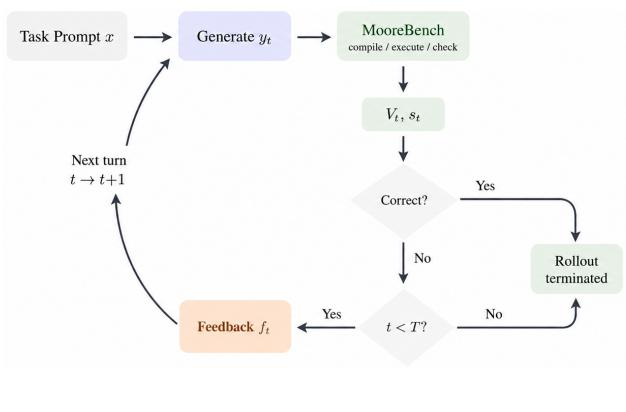
\includegraphics[keepaspectratio,alt={image}]{images/2e90c0c39bb94a7151d053fc1a4f19a9e9791d3454f27855357734cf1e275875.jpg}}

Figure 4: Multi-turn RL rollout process.

\pandocbounded{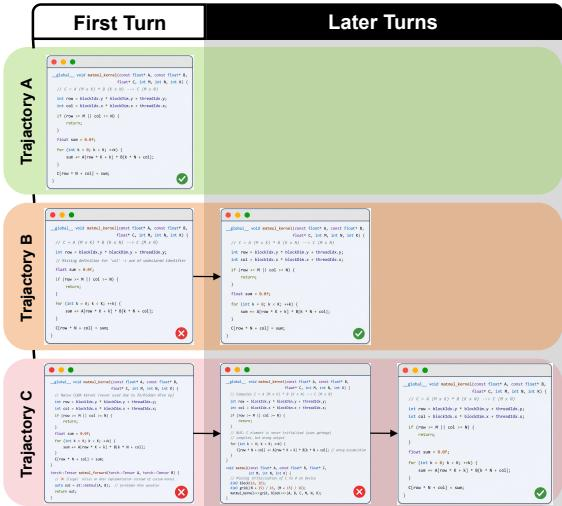
\includegraphics[keepaspectratio,alt={image}]{images/420a2604919bd212f86ac12b11c79aa468dad1277615bfb9cab24d0ab9bcb594.jpg}}

Figure 5: Multi-turn reward design.

Here, \(y _ { i , k }\) denotes the model output at turn
\(k , c _ { i , k }\) the extracted candidate, \(V _ { i , k }\) the
MooreEval verification telemetry, \(s _ { i , k }\) the scalar reward,
and \(f _ { i , k }\) the aggregated textual feedback. The rollout
ceases upon successful verification or when the iteration limit is
exhausted.

The objective of multi-turn rollout is to cultivate the model's capacity
for agentic, iterative coding rather than merely optimizing for
final-turn success. For complex kernel tasks, a model may struggle to
simultaneously satisfy compilation, correctness, legitimacy, and
performance constraints in the first pass. The execution feedback from
MooreEval enables the model to systematically rectify compilation
errors, shape/dtype mismatches, numerical deviations, and suboptimal
implementations.

However, the quality of the first-turn generation remains paramount.
While multi-turn inference improves final success rates, each
interaction turn incurs additional compilation, execution, and
verification latency. If the model can generate a correct and efficient
native kernel in the first attempt, it drastically reduces inference
overhead. Therefore, our goal is to enhance the model's rectification
capabilities without fostering over-reliance on environmental feedback.
Directly optimizing for the final-turn or best-turn reward would
inherently bias the model toward multi-turn success, incentivizing
weaker first-turn generation followed by heavy reliance on subsequent
MooreEval feedback for rectification.

To mitigate this objective drift, we introduce PrimeEcho, a
first-turn-anchored multi-turn reward mechanism. It recontextualizes
multi-turn feedback not as the sole target for final success, but as a
supplementary exploration signal for first-turn generation. By
leveraging the rectification traces revealed in subsequent turns while
maintaining primary optimization pressure on first-turn generation,
PrimeEcho achieves a balanced equilibrium between agentic multi-turn
rectification proficiency and the low-latency efficiency of
first-attempt kernel synthesis

\subsection{4.4.3 PRIMEECHO: FIRST-TURN-ANCHORED MULTI-TURN
REWARD}\label{primeecho-first-turn-anchored-multi-turn-reward}

The core philosophy of PrimeEcho is to explicitly decouple the initial
generation quality from subsequent rectification gains within the
trajectory-level reward. Given a group of G multi-turn trajectories
\(\{ \tau _ { i } \} _ { i = 1 } ^ { G }\) sampled for a single prompt,
let \(c _ { i , k }\) denote the candidate code at turn k for the i-th
trajectory, and let
\(\begin{array} { r } { s _ { i , k } = s ( c _ { i , k } ) } \end{array}\)
) denote its corresponding MooreEval score. We define the
trajectory-level reward as:

\[
R _ {\tau_ {i}} = \alpha s _ {i, 1} + (1 - \alpha) \max _ {1 \leq k \leq K} s _ {i, k} + b _ {\mathrm{early}} (\tau_ {i})\tag{9}
\]

where \(s _ { i , 1 }\) represents the score of the first-turn
generation, max
\(\boldsymbol { 1 } \le \boldsymbol { k } \le \boldsymbol { K } \ S _ { i , k }\)
represents the peak score achieved across the entire multi-turn
interaction, and \(\alpha \in [ 0 , 1 ]\) dictates the emphasis placed
on the initial performance. A larger α skews the training closer to
single-turn RL, whereas a smaller α permits the subsequent rectification
outcomes to provide a stronger auxiliary signal.

The early-success bonus
\(b _ { \mathrm { e a r l y } } ( \tau _ { i } )\) exclusively rewards
initial successes achieved within the first two turns, thereby
incentivizing the model to synthesize a correct solution as
expeditiously as possible. Specifically, let success
\(\left( c _ { i , k } \right)\)

denote an indicator function representing whether the candidate code
\(c _ { i , k }\) passes MooreEval verification. The bonus is formulated
as:

\[
b _ {\text { early }} (\tau_ {i}) = \beta_ {1} \mathbf {1} [ \text { success } (c _ {i, 1}) ] + \beta_ {2} \mathbf {1} [ \neg \text { success } (c _ {i, 1}) \land \text { success } (c _ {i, 2}) ]\tag{10}
\]

where \(\beta _ { 1 } > \beta _ { 2 } \ge 0\) . This term guarantees
that among trajectories that ultimately succeed, those achieving success
earlier accumulate higher rewards.

Formally, PrimeEcho interpolates between a strict first-turn reward and
a best-turn reward:

\[
\alpha = 1 \Rightarrow R _ {\tau_ {i}} = s _ {i, 1} + b _ {\mathrm{early}} (\tau_ {i}), \qquad \alpha = 0 \Rightarrow R _ {\tau_ {i}} = \max _ {1 <   k <   K} s _ {i, k} + b _ {\mathrm{early}} (\tau_ {i})\tag{11}
\]

Thus, α explicitly governs the trade-off between first-turn generation
quality and multi-turn rectification signals. By default, we adopt a
relatively large \(\alpha ,\) ensuring that multi-turn feedback serves
predominantly as a supplementary exploration signal during training,
rather than eclipsing the primary objective of first-turn generation.

Finally, for multiple trajectories generated under the same prompt, we
utilize \(R _ { \tau _ { i } }\) to compute the intra-group normalized
advantage:

\[
\hat {A} _ {i} = \frac {R _ {\tau_ {i}} - \mathrm{mean} (\{R _ {\tau_ {j}} \} _ {j = 1} ^ {G})}{\mathrm{std} (\{R _ {\tau_ {j}} \} _ {j = 1} ^ {G}) + \epsilon}\tag{12}
\]

This formulation is structurally identical to the response-level
advantage in single-turn GRPO, substituting the singleturn reward with
the PrimeEcho trajectory reward. As illustrated in Figure 5, we
predominantly apply this advantage to the tokens comprising the
first-turn output, effectively subordinating the multi-turn feedback to
serve the enhancement of first-turn generation.

\subsection{4.5 RL STABILIZATION
TECHNIQUES}\label{rl-stabilization-techniques}

While MooreEval enables RL training to directly optimize compilation
success, numerical correctness, and runtime performance, execution-based
RL still faces two major stability challenges in practice. First,
complex kernelgeneration tasks frequently produce an all-failed group,
where all candidate implementations sampled for the same prompt fail to
obtain a positive reward. In group-relative optimization, such groups
provide little discriminative learning signal, since the intra-group
advantages cannot reliably distinguish useful directions for policy
improvement. Second, off-policy drift can arise between the rollout
policy used to generate samples and the policy being updated during
training. If left uncontrolled, severely off-policy samples can increase
gradient variance and induce unstable or biased policy updates.

To address these challenges, we introduce two complementary
stabilization components. Buffered Dynamic Retry (BDR) strengthens
learning signals on hard samples by converting all-failed groups into
feedback-conditioned retry tasks, while MirrorPop improves training
stability by identifying and masking high-risk off-policy samples at the
sequence level.

\subsection{4.5.1 BUFFERED DYNAMIC RETRY}\label{buffered-dynamic-retry}

During RL training with GRPO, G candidate implementations are typically
sampled for a given prompt x, and the advantage is computed based on
intra-group rewards. However, for challenging kernel generation tasks,
an all-failed group frequently emerges, wherein all candidate solutions
fail:

\[
r _ {i} = - 1 \quad \text { for   any } 1 \leq i \leq G\tag{13}
\]

Within such an all-failed group, the absence of correct positive samples
deprives the intra-group rewards of meaningful discriminability, failing
to provide a valid optimization direction. Consequently, the model
repeatedly samples failed implementations on long-tail, difficult tasks.
Furthermore, our empirical observations indicate that the most prevalent
failure modes during both the training phase and on the validation set
are verification errors (i.e., kernel precision inaccuracies) and
runtime exceptions (i.e., execution bugs). Therefore, a transitional
training mechanism bridging single-turn and multi-turn RL is
important---one designed to exclusively target these formidable
challenges with minimal training overhead. To this end, we propose
Buffered Dynamic Retry (BDR), which dynamically transfigures these hard
samples into feedback-conditioned rectification tasks, thereby
recovering actionable training signals.

An auxiliary motivation for this mechanism is to investigate whether
empowering the model to rectify its own errors can simultaneously
elevate its first-turn generation capability (i.e., zero-shot code
generation). In practical implementation, the core of the multi-turn
training described later serves primarily to provide exploration
signals; during policy updates, only the first-turn tokens are subjected
to optimization. This is done to prevent the degradation of first-turn
generation quality, though it inherently sacrifices the direct
enhancement of the model's bug-rectification capabilities. Conversely,
BDR considers all tokens during updates. It explicitly trains the model
to reflect upon and rectify errors, internalizing the root causes of
failures. This allows us to explore whether combining BDR with
subsequent multiturn training can augment the model's intrinsic CUDA
domain knowledge without compromising first-turn generation efficacy.

Specifically, given a training dataset
\(\mathcal { D } _ { \mathrm { R L } }\) , upon the conclusion of each
rollout epoch, we scan the MooreEval telemetry within the current batch
to isolate all-failed prompts. For each hard prompt, the system selects
a representative erroneous candidate \(c ^ { - }\) and extracts the
structured error telemetry returned by MooreEval---such as correctness
errors, runtime exceptions, compilation failures, or forbidden aten::*
fallbacks. Subsequently, we concatenate the original task description,
the failed code, and the error feedback into a feedback-conditioned
prompt:

\[
x ^ {\prime} = \mathrm{Compose} (x, c ^ {-}, f ^ {-})\tag{14}
\]

where \(f ^ { - }\) denotes the error summary or rectification hint
automatically synthesized by MooreEval. In doing so, an originally
intractable zero-shot generation task is structurally transformed into a
feedback-driven code rectification task, significantly easing the
model's exploration toward a correct trajectory.

To prevent these feedback-augmented samples from distorting the primary
task distribution, we refrain from immediately replacing the original
training data. Instead, we enqueue \(x ^ { \prime }\) into a dynamic
buffer pool B. The buffer utilizes a First-In-First-Out (FIFO) eviction
policy to constrain its capacity:

\[
\mathcal {B} \leftarrow \text { FIFOUpdate } (\mathcal {B}, x ^ {\prime})\tag{15}
\]

We maintain the buffer at a fixed, predefined capacity. When a new
sample is eligible for insertion and the pool is full, the oldest sample
is evicted. This mechanism ensures the continuous retention of
contemporary hard samples reflecting the model's current failure
boundaries, while purging outdated error trajectories. This is crucial
because the policy model evolves continuously during training; an early
failure sample may no longer pose a challenge in later stages. The FIFO
design mitigates the interference of stale feedback on current policy
updates, guaranteeing that the buffer consistently approximates the
frontier of the model's current capabilities.

In subsequent training iterations, we sample feedback-conditioned
prompts from the buffer pool with a small probability
\(p _ { \mathrm { b u f } }\) , mixing them with prompts from the
original dataset \(\mathcal { D } _ { \mathrm { R L } }\)

\[
x _ {\mathrm{train}} \sim \left\{ \begin{array}{l l} \mathcal {B}, & \text {with probability p_{buf}} \\ \mathcal {D} _ {\mathrm{RL}}, & \text {with probability 1 - p_{buf}} \end{array} \right.\tag{16}
\]

By default, the overwhelming majority of samples continue to originate
from the original single-turn tasks, with only a marginal fraction drawn
from the dynamic buffer. The rationale is that BDR intrinsically
converts a subset of first-turn generation tasks into feedback-driven
rectification tasks. If deployed extensively or during the early stages
of training, it could introduce task interference, fostering an
over-reliance on feedback and subsequently eroding the first-turn
generation capabilities. Thus, we primarily activate this mechanism
during the later stages of RL, deploying it as a stabilization protocol
to conquer long-tail hard samples rather than as a substitute for the
primary single-turn training objective.

Crucially, we rely exclusively on the native execution feedback returned
by MooreEval to guide retries, deliberately avoiding explicit rewriting
prompts generated by external, more capable models. While external
models can synthesize more articulate natural language explanations,
such feedback frequently diverges from the data distribution established
during the SFT phase. This divergence risks introducing
out-of-distribution (OOD) contexts, precipitating entropy fluctuations
and policy instability during training. By contrast, native sandbox
feedback originates directly from the actual execution environment; it
is structurally stable, reproducible, and seamlessly aligns with the
authentic feedback the model will encounter in the subsequent multi-turn
RL phase.

\subsection{4.5.2 MIRRORPOP OFF-POLICY SEQUENCE
MASKING}\label{mirrorpop-off-policy-sequence-masking}

In addition to reward sparsity, off-policy mismatch is another major
source of instability in RL training. During training, the rollout
policy used to generate samples may diverge from the current policy
being optimized. Such drift can arise from train--inference backend
discrepancies, policy changes introduced by reusing the same rollout
batch across multiple mini-batch updates, or discrete distributional
shifts caused by routing perturbations in MoE models. When the mismatch
becomes severe, the resulting importance ratios can produce
high-variance gradient estimates and unstable policy updates. Therefore,
it is important to identify and filter high-risk samples that deviate
substantially from the rollout policy.

A straightforward way to control off-policy updates is to apply
token-level clipping or hard filtering to the importance ratio
\(\rho _ { i , t }\) , as in Truncated Importance Sampling (TIS) (Yao et
al., 2025) and IcePop (Zhao et al., 2025). However, similar to
token-level PPO clipping (Schulman et al., 2017), such methods operate
on individual tokens and therefore do not directly capture whether an
entire response has drifted substantially from the rollout distribution
(Li et al., 2026). This limitation is particularly relevant for
long-form kernel generation, where moderate token-level deviations can
accumulate into a severe sequence-level mismatch.

To address this issue, sequence-level masking introduces a binary mask
\(M _ { i } \in \{ 0 , 1 \}\) for each response. When \(M _ { i } = 0\)
the entire response is excluded from the policy-gradient update; when
\(M _ { i } = 1\) , the response is retained and contributes normally to
optimization. The GRPO objective augmented with sequence-level masking
is then formulated as:

\[
\mathcal {L} _ {\mathrm{GRPO-mask}} (\theta) = - \frac {1}{\sum_ {i = 1} ^ {G} M _ {i} L _ {i}} \sum_ {i = 1} ^ {G} \sum_ {t = 1} ^ {L _ {i}} \min \left(\rho_ {i, t} (\theta) \hat {A} _ {i}, \operatorname{clip} \left(\rho_ {i, t} (\theta), 1 - \epsilon_ {\text {low}}, 1 + \epsilon_ {\text {high}}\right) \hat {A} _ {i}\right) M _ {i} + \beta D _ {\mathrm{KL}} \left(\pi_ {\theta} \| \pi_ {\text {ref}}\right)\tag{17}
\]

The key design question is how to determine the response-level mask
\(M _ { i }\) . A common sequence-level off-policy masking strategy
defines a response-level importance ratio using the length-normalized
geometric mean of token-level ratios (Liu et al., 2025b;a):

\[
\bar {\rho} _ {i} ^ {\mathrm{geo}} = \left(\prod_ {t = 1} ^ {L _ {i}} \rho_ {i, t}\right) ^ {1 / L _ {i}} = \exp \left(\frac {1}{L _ {i}} \sum_ {t = 1} ^ {L _ {i}} \log \rho_ {i, t}\right)\tag{18}
\]

The sequence is then retained or discarded according to whether
\(\bar { \rho } _ { i } ^ { \mathrm { g e o } }\) falls within a
predefined trust interval. However, this geometric-mean statistic is
equivalent to exponentiating the signed mean log-ratio, and therefore
suffers from directional cancellation. For example, consider two tokens
with importance ratios \(\rho _ { 1 } ~ = ~ 1 0\) and
\(\rho _ { 2 } ~ = ~ 0 . 1\) . Both tokens exhibit large deviations from
the rollout policy, but their signed log-ratio deviations cancel: log
\(\rho _ { 1 } + \log \rho _ { 2 } =\) log \(1 0 + \log { 0 . 1 } = 0\)
. As a result, the corresponding geometric mean becomes close to 1,
causing the conventional sequence-level mask to regard the response as
nearly on-policy. This judgment is misleading: an over-weighted token
and an under-weighted token offset each other algebraically in log
space, but such cancellation does not imply that the sequence is safe
for training.

Figure 11 illustrates this effect with a real example. Red and green
tokens denote positive and negative log-ratio deviations, respectively.
When log \(\rho _ { t }\) is directly accumulated or averaged across the
sequence, deviations with opposite signs can cancel, obscuring the true
magnitude of sequence-level policy mismatch. In severe cases, a response
containing strong local deviations may still appear nearly on-policy
under the signed statistic. For off-policy filtering, however, the
relevant quantity is the magnitude of deviation from the rollout policy
rather than its signed direction. Thus, signed aggregation can
underestimate the risk of high-mismatch trajectories.

To address this cancellation problem, we propose MirrorPop. Instead of
distinguishing whether a token is assigned a higher or lower probability
by the current policy than by the rollout policy, MirrorPop measures the
direction-invariant magnitude of the deviation. For each token, we
define the mirror deviation as:

\[
m _ {i, t} = \max (\rho_ {i, t}, \rho_ {i, t} ^ {- 1}) = \exp (| \log \rho_ {i, t} |), \qquad m _ {i, t} \geq 1\tag{19}
\]

This formulation is symmetric with respect to reciprocal ratios: both
\(\rho _ { i , t } = 1 0\) and \(\rho _ { i , t } = 0 . 1\) are mapped
to the same deviation magnitude, since max
\(( 1 0 , 1 / 1 0 ) = \operatorname* { m a x } ( 0 . 1 , 1 / 0 . 1 ) = 1 0\)
. Aggregating this direction-invariant deviation over the response, we
define the length-normalized MirrorPop statistic as:

\[
\bar {m} _ {i} ^ {\mathrm{geo}} = \left(\prod_ {t = 1} ^ {L _ {i}} \max (\rho_ {i, t}, \rho_ {i, t} ^ {- 1})\right) ^ {1 / L _ {i}} = \exp \left(\frac {1}{L _ {i}} \sum_ {t = 1} ^ {L _ {i}} | \log \rho_ {i, t} |\right)\tag{20}
\]

The corresponding sequence-level mask is thus defined as:

\[
M _ {i} ^ {\mathrm{mirrorpop}} = \mathbf {1} \left[ \frac {1}{L _ {i}} \sum_ {t = 1} ^ {L _ {i}} | \log \rho_ {i, t} | \leq \delta \right]\tag{21}
\]

where δ denotes the threshold in log-ratio space.

The key distinction between MirrorPop and conventional sequence-level
masking lies in how token-level ratios are aggregated. Conventional
masking relies on the signed average
\(\begin{array} { r } { \frac { 1 } { L _ { i } } \sum _ { t } \log \rho _ { i , t } , } \end{array}\)
, whereas MirrorPop uses the absolutedeviation average
\(\begin{array} { r } { \frac { 1 } { L _ { i } } \sum _ { t } | \log \rho _ { i , t } | } \end{array}\)
. As a result, positive and negative deviations no longer cancel;
instead, both contribute to the sequence-level mismatch score.
Revisiting the example \(\rho ~ = ~ [ 1 0 , 0 . 1 ]\) , the conventional
signed statistic gives
\(\frac { 1 } { \cdot } ( \log \dot { 1 } 0 + \log 0 . 1 ) = 0\) ,
corresponding to a geometric mean ratio of 1. In contrast, MirrorPop
gives
\(\begin{array} { r } { \frac { 1 } { 2 } ( | \log 1 0 | + | \mathbf { \bar { l } } \log 0 . 1 | ) = \log 1 0 } \end{array}\)
, equivalently assigning a ratio-space mismatch magnitude of 10. Thus,
MirrorPop correctly identifies the response as a high-risk off-policy
sample.

In RL training with GRPO, we use
\(M _ { i } = M _ { i } ^ { \mathrm { m i r r o r p o p } }\) as the
response-level masking criterion. MirrorPop complements token-level
ratio clipping by operating at a different granularity: token-level
clipping limits the update contribution of individual tokens, whereas
MirrorPop determines whether the entire response has drifted too far
from the rollout policy to be safely used for optimization. In this
sense, MirrorPop measures ``how
\(\mathrm { f a r } ^ { \prime \prime }\) a response deviates from the
rollout policy, rather than ``in which direction'' it deviates. This
magnitude-based sequence filtering mitigates the underestimation caused
by signed log-ratio cancellation, enabling more reliable removal of
severely off-policy samples and improving the stability of RL updates.

\subsection{5 EXPERIMENTS}\label{experiments}

\subsection{5.1 TRAINING DETAILS}\label{training-details}

During the supervised training phase, we fine-tune two base checkpoints:
MusaCoder-9B is initialized from Qwen3.5- 9B1, and MusaCoder-27B is
initialized from Qwen3.6-27B2. Unless otherwise specified, both model
scales follow the same training pipeline. We use the AdamW(Loshchilov
and Hutter, 2017) optimizer with a learning rate of
\(1 \times 1 0 ^ { - 5 }\) a warmup ratio of 3\%, weight decay of 0.01,
and bf16 precision. The maximum sequence length is set to 40K, and the
global batch size is 256, training for 1 epoch. For multi-turn SFT
samples, we apply the loss masking strategy detailed in Section 4.2.3:
historical turns serve exclusively as contextual input, and the loss is
computed solely on the model's final-turn response. The SFT
implementation is built on DeepSpeed, incorporating ZeRO/offload
techniques to support long-context supervised fine-tuning(Rajbhandari et
al., 2020).

The reinforcement learning phase employs a two-stage GRPO pipeline. The
first stage, single-turn GRPO, aims to enhance the model's capacity to
directly generate correct, legal, and efficient kernels under
zero-feedback conditions. The second stage proceeds from the single-turn
checkpoint into multi-turn RL, introducing online feedback from
MooreEval as a rectification signal for subsequent turns. A multi-turn
rollout spans a maximum of 3 model response turns; the trajectory
terminates early if a candidate implementation passes verification at
any turn.

Across both RL stages, the rollout group size is set to 8, with a
training batch size of 64. Rollouts are executed using SGLang in async
mode. The training sampling parameters are temperature 0.9 and top-
\(\cdot p = 0 . 9 5\) , while validation sampling uses temperature 0.7
and \(\mathrm { t o p } { - } p ~ = ~ 0 . 7\) . Multi-turn RL employs
the PrimeEcho reward with \(\alpha = 0 . 7 5\) by default. Notably,
multi-turn RL calculates the policy gradient loss exclusively on the
first-turn model response; subsequent turns participate only in
trajectory evaluation and reward computation.

The RL training infrastructure is built on Megatron + SGLang(Shoeybi et
al., 2019; Zheng et al., 2024), where Megatron manages the distributed
training of the actor and reference models, and SGLang handles
high-throughput asynchronous rollouts. Tensor parallelism is introduced
to distribute model parameters and mitigate activation memory overhead,
especially for the 27B model. The RL learning rate is set to
\(1 \times 1 0 ^ { - 6 }\) , with a warmup ratio of 0.1, weight decay of
0.1, and gradient clipping at 0.5. The maximum prompt length is 8K, and
the maximum response length is 32K.

All experiments are conducted on 64 Moore Threads MTT S5000 machines,
each equipped with \(8 \times 8 0 \mathrm { G B }\) accelerator cards3.
This cluster robustly sustains the end-to-end training loop,
encompassing long-context SFT, asynchronous rollouts, MooreEval online
verification, and GRPO policy updates. Specifically, executing both
supervised fine-tuning and execution-feedback reinforcement learning for
9B and 27B models on this domestic hardware environment demonstrates
that the platform can support not only standard LLM fine-tuning but also
complex RL training workloads involving large-scale code generation,
compile-and-execute feedback, and online reward computation.

\subsection{5.2 EVALUATION SETUP}\label{evaluation-setup}

We evaluate MusaCoder's PyTorch-to-CUDA/MUSA kernel generation
capabilities on the KernelBench benchmark, employing the unified
MooreEval protocol to validate all models. Unlike the original
evaluation scripts, we strictly require candidate implementations to
successfully parse and compile, pass shape, dtype, and numerical
correctness checks against the PyTorch reference on randomized inputs,
and refrain from invoking forbidden PyTorch/aten::* computational
fallbacks within ModelNew.forward(). Only candidate implementations that
pass both correctness and legality checks proceed to performance
testing. Performance measurements are conducted using repeated runs
after warmup and timed via synchronized CUDA events to reduce variance
from asynchronous execution and initialization overhead.

For each task, we sample 8 candidate implementations at temperature 0.7
and report two categories of metrics. Pass Rate measures correctness.
Pass@8 indicates whether at least one of the 8 sampled candidates passes
MooreEval verification, while Avg.@8 reports the average fraction of
verified candidates among the 8 samples. Faster Rate measures
performance improvement among valid native kernel implementations. A
candidate is counted as faster only if it first passes correctness and
legality checks and then achieves a runtime speedup larger than 1.1×
over the corresponding baseline. We report Faster Rate against both
PyTorch eager execution and torch.compile. The 1.1× threshold filters
out marginal runtime differences that may arise from measurement noise.

We compare MusaCoder with both frontier code models and its underlying
base models. The external baselines include Claude Opus 4.7, GLM-5.1,
Kimi K2.6, and DeepSeek-V4-Pro/ProMax. We also report Qwen3.5-9B and
Qwen3.6-27B to quantify the improvement brought by MusaCoder's SFT/RFT
and RL pipeline over the initial base checkpoints. All models are
evaluated under identical prompt templates, sampling configurations,
validation scripts, and hardware environments. Unless otherwise
specified, all main results are reported across Overall, Level 1, Level
2, and Level 3 categories.

\subsection{5.3 MAIN RESULTS ON
KERNELBENCH}\label{main-results-on-kernelbench}

Table 1 reports the main KernelBench results under the strict MooreEval
protocol. In addition to frontier code models, we also include the two
base checkpoints, Qwen3.5-9B and Qwen3.6-27B, to quantify the
improvement brought by MusaCoder's training pipeline. All models are
evaluated with the same prompts, sampling configuration, verifier, and
hardware environment.

The base models show limited native kernel generation ability under
strict executable verification. Qwen3.5-9B obtains only 23.6\% Overall
Pass@8 and 7.05\% Avg.@8, while Qwen3.6-27B improves to 67.2\% Pass@8
and 35.60\% Avg.@8 but still falls behind strong general-purpose code
models. After supervised alignment, MusaCoder-9B-SFT increases Overall
Pass@8 to 69.6\% and Avg.@8 to 61.60\%, while MusaCoder-27B-SFT reaches
84.8\% and 79.40\%. These results indicate that the proposed SFT/RFT
data pipeline substantially improves both task-format following and
single-sample correctness stability.

Execution-feedback RL further improves both model scales.
MusaCoder-9B-RL raises Overall Pass@8 from 69.6\% to 83.6\% and Avg.@8
from 61.60\% to 77.20\%, approaching Claude Opus 4.7 in correctness
under the same strict verifier. For the larger model, MusaCoder-27B-RL
achieves the best overall correctness, reaching 93.2\% Pass@8 and
88.60\% Avg.@8. Compared with Claude Opus 4.7, this corresponds to
absolute gains of 6.0 points in Pass@8 and 11.30 points in Avg.@8. The
advantage is more pronounced on Level 3, where MusaCoder-27B-RL improves
Pass@8 from Claude's 54\% to 72\% and Avg.@8 from 39.25\% to 65.75\%,
suggesting stronger robustness on complex shape reasoning, indexing, and
multi-operator workloads.

Faster Rate is more stringent than correctness because a candidate is
counted only when it is correct, legal, and achieves more than 1.1×
speedup over the corresponding PyTorch baseline. Under this criterion,
the base models rarely produce accelerated kernels: Qwen3.5-9B achieves
only 0.9\% Faster Rate vs.~Eager and 0.5\% vs.~Compile, while
Qwen3.6-27B reaches 3.4\% and 1.6\%. MusaCoder-9B-RL already slightly
surpasses Claude Opus 4.7 on performance, achieving 12.6\% vs.~Eager and
7.9\% vs.~Compile, compared with Claude's 11.8\% and 7.5\%.

MusaCoder-27B-RL shows the strongest performance gains, achieving 15.0\%
Faster Rate vs.~Eager and 9.2\% vs.~Compile. These are absolute
improvements of 3.2 and 1.7 points over Claude Opus 4.7. Overall, these
results show that MusaCoder's execution-feedback training improves not
only functional correctness but also the probability of generating
native kernels with measurable runtime benefits.

Table 1: KernelBench evaluation results under the strict MooreEval
protocol. We report correctness-oriented Pass Rate metrics and
performance-oriented Faster Rate metrics across Overall, Level 1, Level
2, and Level 3. Pass@8 denotes whether at least one of 8 sampled
candidates passes verification, while Avg.@8 measures the average
correctness rate among the 8 samples. Faster Rate is reported against
PyTorch eager execution (Paszke et al., 2019) and torch.compile (Ansel
et al., 2024); a candidate is counted as faster only if it passes
correctness and legality checks and achieves speedup larger than 1.1×
over the corresponding baseline.

{\def\LTcaptype{none} % do not increment counter
\begin{longtable}[]{@{}lllllllll@{}}
\toprule\noalign{}
\endhead
\bottomrule\noalign{}
\endlastfoot
\multirow{2}{*}{Model} & \multicolumn{2}{l}{%
Overall} & \multicolumn{2}{l}{%
Level 1} & \multicolumn{2}{l}{%
Level 2} & \multicolumn{2}{l@{}}{%
Level 3} \\
& Pass@8 & Avg.@8 & Pass@8 & Avg.@8 & Pass@8 & Avg.@8 & Pass@8 &
Avg.@8 \\
Kimi K2.6 & 84.0 & 69.10 & 94 & 77.13 & 89 & 75.50 & 54 & 40.25 \\
GLM-5.1 & 85.6 & 76.25 & 98 & 89.38 & 89 & 82.00 & 54 & 38.50 \\
DeepSeek-V4-Pro & 83.2 & 54.90 & 97 & 68.88 & 86 & 56.38 & 50 & 24.00 \\
DeepSeek-V4-ProMax & 84.8 & 60.05 & 97 & 72.88 & 92 & 62.63 & 46 &
29.25 \\
Claude Opus 4.7 & 87.2 & 77.30 & 99 & 91.75 & 92 & 81.88 & 54 & 39.25 \\
Qwen3.5-9B & 23.6 & 7.05 & 35 & 11.63 & 22 & 5.75 & 4 & 0.50 \\
Qwen3.6-27B & 67.2 & 35.60 & 83 & 44.38 & 68 & 36.13 & 34 & 17.00 \\
MusaCoder-9B-SFT & 69.6 & 61.60 & 88 & 79.88 & 71 & 63.50 & 30 &
21.25 \\
MusaCoder-9B-RL & 83.6 & 77.20 & 94 & 89.25 & 89 & 84.50 & 52 & 38.50 \\
MusaCoder-27B-SFT & 84.8 & 79.40 & 95 & 89.00 & 92 & 87.75 & 50 &
43.50 \\
MusaCoder-27B-RL & 93.2 & 88.60 & 99 & 95.75 & 98 & 92.88 & 72 &
65.75 \\
\multicolumn{9}{@{}l@{}}{%
} \\
\multirow{2}{*}{Model} & \multicolumn{2}{l}{%
Overall} & \multicolumn{2}{l}{%
Level 1} & \multicolumn{2}{l}{%
Level 2} & \multicolumn{2}{l@{}}{%
Level 3} \\
& vs. Eager & vs. Compile & vs. Eager & vs. Compile & vs. Eager & vs.
Compile & vs. Eager & vs. Compile \\
Kimi K2.6 & 3.3 & 1.4 & 7.5 & 3.0 & 0.6 & 0.5 & 0.2 & 0.0 \\
GLM-5.1 & 7.4 & 3.9 & 14.3 & 6.0 & 3.8 & 3.6 & 1.0 & 0.0 \\
DeepSeek-V4-Pro & 5.2 & 3.0 & 10.3 & 4.8 & 2.8 & 2.6 & 0.0 & 0.0 \\
DeepSeek-V4-ProMax & 5.7 & 3.0 & 11.6 & 5.0 & 2.3 & 2.3 & 0.5 & 0.3 \\
Claude Opus 4.7 & 11.8 & 7.5 & 21.0 & 10.5 & 6.9 & 6.8 & 3.3 & 2.8 \\
Qwen3.5-9B & 0.9 & 0.5 & 2.0 & 1.1 & 0.3 & 0.1 & 0.0 & 0.0 \\
Qwen3.6-27B & 3.4 & 1.6 & 8.3 & 3.6 & 0.3 & 0.3 & 0.0 & 0.0 \\
MusaCoder-9B-SFT & 1.6 & 1.2 & 3.0 & 2.1 & 1.0 & 0.8 & 0.0 & 0.0 \\
MusaCoder-9B-RL & 5.4 & 3.2 & 9.8 & 5.0 & 3.3 & 2.9 & 0.7 & 0.4 \\
MusaCoder-27B-SFT & 6.3 & 4.1 & 12.1 & 7.6 & 3.0 & 2.2 & 1.3 & 1.0 \\
MusaCoder-27B-RL & 15.0 & 9.2 & 25.7 & 12.8 & 10.2 & 8.7 & 3.2 & 3.0 \\
\end{longtable}
}

\subsection{5.4 ABLATION AND RL TRAINING
ANALYSIS}\label{ablation-and-rl-training-analysis}

To systematically deconstruct the contributions of individual training
components within MusaCoder, we conduct rigorous ablation studies and
training dynamics analyses across the supervised phase, the
reinforcement learning phase, and the RL stabilization mechanisms.
Diverging from the main experiments---which merely report the terminal
KernelBench benchmarks---this section explicitly decouples first-turn
generation, multi-turn repair, reward dynamics, and training stability
to illuminate the precise origins of the model's performance gains.

\subsection{5.4.1 EVALUATION METRICS FOR MULTI-TURN
RL}\label{evaluation-metrics-for-multi-turn-rl}

To clearly delineate the model's zero-shot generation capability from
its multi-turn feedback-driven rectification proficiency, we report both
first-turn metrics and best-turn metrics concurrently during multi-turn
evaluation. For the i-th validation sample, let \(c _ { i , t }\) denote
the candidate code generated at turn t, and let its corresponding
MooreEval score be \(s _ { i , t }\) . We define the binary success
indicator function as:

\[
\mathrm{success} (c _ {i, t}) = \mathbf {1} [ s _ {i, t} \geq 1 ]\tag{22}
\]

First-turn accuracy measures the model's capability to correctly
synthesize a kernel in a single attempt, strictly under zero-feedback
conditions:

\[
\mathrm{Acc} _ {\mathrm{first}} = \frac {1}{N} \sum_ {i = 1} ^ {N} \mathrm{success} (c _ {i, 1})\tag{23}
\]

This metric directly proxies the model's performance in standard
single-turn deployment scenarios, thus acting as one of the most
critical constraint metrics during multi-turn RL optimization.

Best-turn accuracy measures whether the model can ultimately rectify a
failure within a maximum horizon of T feedback turns:

\[
\mathrm{Acc} _ {\mathrm{best}} = \frac {1}{N} \sum_ {i = 1} ^ {N} \max _ {1 \leq t \leq T} \mathrm{success} (c _ {i, t})\tag{24}
\]

If a specific sample fails on the first attempt but is successfully
rectified in subsequent turns, it does not positively impact the
first-turn accuracy but directly elevates the best-turn accuracy.
Consequently, the best-turn accuracy primarily reflects the model's
agentic proficiency in leveraging MooreEval feedback for continuous
rectification.

Beyond binary correctness rates, we also report the first-turn score and
best-turn score:

\[
S _ {\mathrm{first}} = \frac {1}{N} \sum_ {i = 1} ^ {N} s _ {i, 1}, \qquad S _ {\mathrm{best}} = \frac {1}{N} \sum_ {i = 1} ^ {N} \max _ {1 \leq t \leq T} s _ {i, t}\tag{25}
\]

The scalar score preserves granular telemetry---such as partial
correctness shaping, structural infraction penalties, and empirical
speedup bonuses---rendering it a higher-resolution metric than binary
accuracy. Finally, we aggregate the turn-to-success (i.e., the specific
turn number at which a sample first passes verification) to empirically
observe whether the policy exhibits a distributional bias toward
immediate zero-shot success or an over-reliance on deferred
feedback-driven rectifications.

\subsection{5.4.2 COMPONENT ABLATION}\label{component-ablation}

Table 2 reports the ablation results for the main training components.
Overall, each component contributes to the final performance, but their
effects are reflected in different aspects: RFT improves supervised task
alignment, single-turn warmup provides a stronger initialization for
multi-turn RL, PrimeEcho controls the multi-turn reward objective, BDR
recovers learning signals from hard samples, and MirrorPop stabilizes
off-policy updates.

Table 2: Ablation study on the main training components. We report
Overall Pass Rate and Faster Rate to measure the effect of each
component on correctness and performance.

{\def\LTcaptype{none} % do not increment counter
\begin{longtable}[]{@{}lllll@{}}
\toprule\noalign{}
\endhead
\bottomrule\noalign{}
\endlastfoot
\multirow{2}{*}{Setting} & \multicolumn{2}{l}{%
Overall Pass Rate} & \multicolumn{2}{l@{}}{%
Overall Faster Rate} \\
& Pass@8 & Avg.@8 & vs. Eager & vs. Compile \\
MusaCoder-SFT & 84.8 & 79.40 & 6.3 & 4.1 \\
w/o RFT & 82.6 & 75.10 & 5.8 & 3.8 \\
MusaCoder-RL & 93.2 & 88.60 & 15.0 & 9.2 \\
w/o Single-turn Warmup & 90.8 & 84.25 & 14.2 & 8.6 \\
w/o PrimeEcho & 88.4 & 83.50 & 13.9 & 8.4 \\
w/o Buffered Dynamic Retry & 88.6 & 83.20 & 13.8 & 8.2 \\
w/o MirrorPop & 86.0 & 80.75 & 13.1 & 7.8 \\
\end{longtable}
}

First, RFT improves the supervised checkpoint before RL. Removing RFT
reduces MusaCoder-SFT's Overall Pass@8 from 84.8\% to 82.6\% and Avg.@8
from 79.40\% to 75.10\%, corresponding to drops of 2.2 and 4.30
percentage points. The performance metrics also decline: Faster Rate
vs.~Eager decreases from 6.3\% to 5.8\%, and vs.~Compile decreases from
4.1\% to 3.8\%. This indicates that MooreEval-filtered RFT improves not
only correctness but also the stability of single-sample generation.
Since our RFT uses diversity-preserving filtering rather than selecting
only the fastest candidate, it strengthens task alignment while
maintaining implementation diversity for downstream RL exploration.

Second, single-turn warmup is important for initializing the multi-turn
RL stage. Without single-turn warmup, MusaCoder-RL drops from 93.2\% to
90.8\% in Overall Pass@8 and from 88.60\% to 84.25\% in Avg.@8. The
Faster Rate also decreases substantially, from 15.0\% to 14.2\% against
PyTorch eager execution and from 9.2\% to 8.6\% against torch.compile.
These results suggest that directly entering multi-turn RL from the
supervised checkpoint weakens the training signal, because early
feedback turns are more likely to be spent on basic formatting,
compilation, or interface errors. Single-turn warmup first aligns the
policy with executable verification, giving the subsequent multi-turn
stage a stronger starting point.

PrimeEcho also brings clear gains. Removing PrimeEcho reduces Overall
Pass@8 from 93.2\% to 88.4\% and Avg.@8 from 88.60\% to 83.50\%. Faster
Rate decreases from 15.0\%/9.2\% to 13.9\%/8.4\% against PyTorch eager
execution and torch.compile, respectively. This confirms the importance
of first-turn-anchored multi-turn reward: if the trajectory reward
over-emphasizes final-turn or best-turn success, the model may rely more
heavily on later feedback instead of improving first-turn generation
quality. PrimeEcho preserves the benefit of multi-turn exploration while
maintaining pressure on the first response.

Buffered Dynamic Retry also contributes noticeably to the final model.
Removing BDR reduces Overall Pass@8 from 93.2\% to 88.6\% and Avg.@8
from 88.60\% to 83.20\%, corresponding to drops of 4.6 and 5.40
percentage points. The Faster Rate decreases from 15.0\%/9.2\% to
13.9\%/8.4\%. Although BDR is designed to target all-failed hard samples
rather than every training example, its ablation still leads to a
sizable degradation, suggesting that recovering learning signals from
long-tail difficult prompts is important for both correctness and
performance.

Finally, MirrorPop has the largest impact among the stabilization
components. Without MirrorPop, Overall Pass@8 drops from 93.2\% to
86.0\%, while Avg.@8 decreases from 88.60\% to 80.75\%, corresponding to
drops of 7.2 and 7.85 percentage points. Faster Rate also falls from
15.0\%/9.2\% to 13.1\%/7.8\%. This demonstrates that off-policy sequence
masking is not merely a background stability trick; it directly affects
final correctness and speedup. By measuring the absolute magnitude of
log-ratio deviations, MirrorPop avoids the cancellation problem of
signed log ratios and filters out high-mismatch sequences that would
otherwise introduce unstable policy updates.

\subsection{5.4.3 EFFECT OF SINGLE-TURN RL
WARMUP}\label{effect-of-single-turn-rl-warmup}

Single-turn RL constitutes the critical transitional phase bridging
supervised learning and execution-feedback opti mization in MusaCoder.
Both the main results and the ablation studies unequivocally demonstrate
that this phase not only elevates terminal metrics but profoundly
ameliorates the initialization quality for subsequent multi-turn
training. Taking the 27B model as a primary example, the Overall Pass@8
and Avg.@8 during the SFT phase stand at 84.8\% and 79.40\%,
respectively. Following RL, these metrics surge to 93.2\% and 88.60\%.
In terms of performance, the Faster Rate vs.~Eager escalates from 6.3\%
to 15.0\%, and vs.~Compile from 4.1\% to 9.2\%. This substantiates that
execution-driven rewards do not merely amplify the probability of
authoring functionally correct kernels; they dramatically inflate the
proportion of kernels that achieve genuine hardware acceleration.

Unlike SFT/RFT---which intrinsically relies on offline static
samples---every candidate implementation synthesized during single-turn
RL is subjected to live, iterative processing by MooreEval. Each
response is compiled, executed, validated for mathematical correctness,
and rigidly inspected for forbidden PyTorch/aten::* fallbacks. Only
after satisfying strict functional and architectural compliance checks
is the candidate benchmarked for relative speedup against the PyTorch
baseline. Consequently, the optimization gradient in this phase
perfectly mirrors the terminal evaluation objective: high rewards are
exclusively minted by native CUDA/MUSA kernels that are compilable,
numerically sound, architecturally legal, and empirically performant.

Analyzing the empirical training trajectory reveals three primary
dimensions of improvement induced by singleturn RL. First, it
systematically eradicates low-level formatting anomalies---such as code
extraction failures, missing ModelNew structural declarations, and
return type mismatches---enforcing an output distribution that stably
adheres to the evaluation interface. Second, MooreEval's draconian
penalization of forbidden fallbacks actively suppresses the model's
inclination to invoke high-level PyTorch/aten::* operators as a shortcut
to bypassing the core task, aggressively steering the policy toward
explicit custom kernel synthesis. Finally, among samples that are
already functionall correct, the continuous performance reward further
stratifies implementation quality. It computationally incentivizes the
model to favor optimal thread mapping, contiguous memory access
patterns, and efficient reduction heuristics, thereby directly elevating
the acceleration ratio among verified kernels.

The ablation results further codify the single-turn warmup as an
indispensable foundational prerequisite for subsequent multi-turn RL.
Ablating the single-turn warmup regresses MusaCoder-RL's Overall Pass@8
from 93.2\% down to 90.8\%, and its Avg.@8 from 88.60\% down to 84.25\%;
the Faster Rate vs.~Compile concurrently drops from 9.2\% to 8.6\%. This
underscores a severe pathology: thrusting a supervised model directly
into multi-turn training forces the system to squander valuable feedback
epochs on rectifying primitive formatting violations and trivial
compilation aborts. By contrast, interposing the single-turn RL phase
ensures that the subsequent multi-turn regime can exclusively focalize
on high-value rectification modes, such as numerical convergence
debugging, boundary condition handling, complex tensor indexing, and
algorithmic performance profiling.

\subsection{5.4.4 TRAINING DYNAMICS OF MULTI-TURN
RL}\label{training-dynamics-of-multi-turn-rl}

Figure 6 illustrates the training dynamics throughout the multi-turn RL
phase. As training progresses, the average number of interaction turns
per sample steadily declines, while the aggregated multi-turn reward
exhibits a continuous upward trajectory. This indicates that the policy
model not only converges toward higher terminal scores across multiturn
interactions but concurrently curtails its over-reliance on deferred
feedback epochs, exhibiting a pronounced inductive bias toward
synthesizing viable candidate solutions in earlier turns. Given the
inherently sparse nature of rewards in kernel generation tasks and the
profound variance in task difficulty, the raw telemetry exhibits
anticipated structural volatility; nonetheless, the smoothed
trajectories delineate a definitive and stable optimization trend.

\pandocbounded{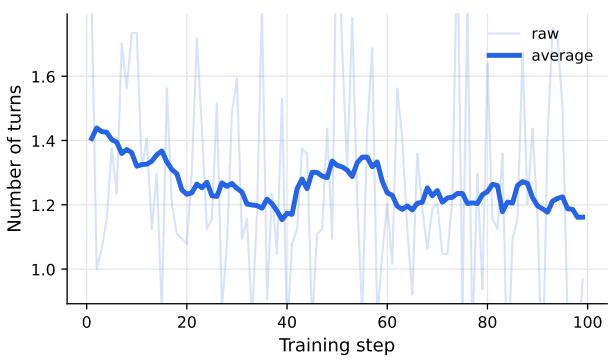
\includegraphics[keepaspectratio,alt={image}]{images/f8eeafc70544e1ef602cab9dbbab4fc550d4629d683ef20300f3f85010869b53.jpg}}

\begin{enumerate}
\def\labelenumi{(\alph{enumi})}
\tightlist
\item
  Number of turns
\end{enumerate}

\pandocbounded{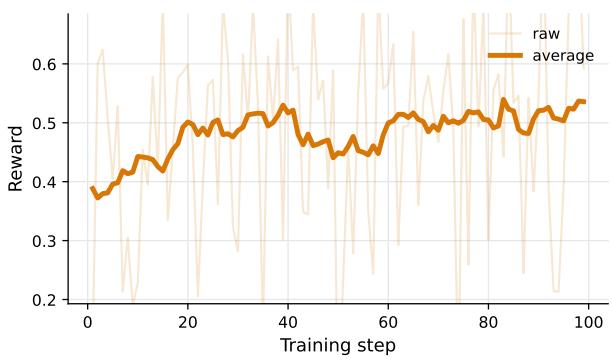
\includegraphics[keepaspectratio,alt={image}]{images/584e93dc776467a2fe6c5a7d15992650d3353e672cb3225ebdc2e448e5f900ba.jpg}}

\begin{enumerate}
\def\labelenumi{(\alph{enumi})}
\setcounter{enumi}{1}
\tightlist
\item
  Reward
\end{enumerate}

Figure 6: Training dynamics of multi-turn reinforcement learning. Raw
curves are shown in light color and smoothed curves are used for
readability.

Figure 7 further decomposes the multi-turn evaluation results across
distinct difficulty tiers. The Score metric proxies the holistic quality
of the model's output, encapsulating partial correctness, architectural
legality, and empirical performance parameters. The Accuracy metric is
concurrently reported for both first-turn and best-turn outcomes,
explicitly isolating zero-shot generation proficiency from multi-turn
rectification capability. The Avg. Eval Turns metric quantifies the mean
number of evaluation iterations required for the model to converge upon
a functionally correct solution.

\pandocbounded{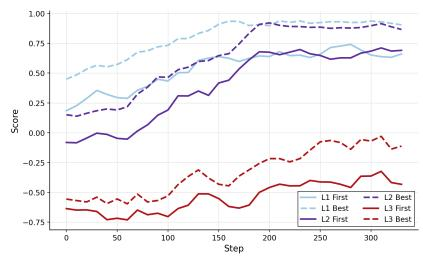
\includegraphics[keepaspectratio,alt={image}]{images/47a08e746efb176f0b10abcadd37f5d78be18ab5f69d02c5f1fc85546cddbee9.jpg}}

Score

\pandocbounded{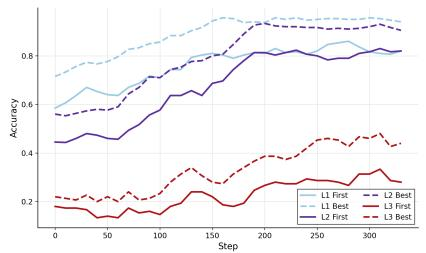
\includegraphics[keepaspectratio,alt={image}]{images/a9bb346af81a1f3851fd894e02282aa5073ce01d73117201a66a8ab563fd2f66.jpg}}

Accuracy

\pandocbounded{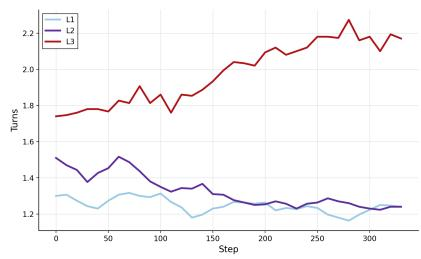
\includegraphics[keepaspectratio,alt={image}]{images/f9602ec325faee86f19a99056b8a9e7ee7fc6492b60bcd8be04fb2753f431a16.jpg}}

Turns

Figure 7: Multi-turn evaluation metrics across KernelBench levels.

Analyzing the disparate difficulty levels reveals that Level 1 tasks
predominantly achieve high correctness rates within the very first turn,
accompanied by a low average evaluation turn count. This suggests that
the model has robustly internalized the heuristics for foundational
operators and trivial composite patterns. Conversely, Level 2 and Level
3 tasks exhibit noticeably lower first-turn accuracies; however, their
best-turn accuracies experience a marked surge following multi-turn
feedback. This confirms that MooreEval feedback fundamentally empowers
the model to debug and rectify complex shape, dtype, indexing, and
numerical convergence errors. Concurrently, the elevated average
evaluation turn count for Level 3 tasks underscores that intricate,
model-level kernels inherently demand protracted feedback horizons to
achieve full rectification.

These empirical dynamics vindicate the architectural rationale
underpinning PrimeEcho. While multi-turn feedback intrinsically elevates
the terminal rectification success rate, optimizing the policy
exclusively for best-turn success risks cultivating an over-reliance on
subsequent feedback, inevitably eroding first-turn zero-shot generation
quality. PrimeEcho mitigates this by rigidly anchoring the trajectory
reward to the initial turn's score, relegating multi-turn feedback to an
auxiliary exploratory signal designed to augment---rather than
eclipse---the primary objective of firstturn generation. The ablation
studies unequivocally validate this: omitting PrimeEcho precipitates a
regression in Overall Avg.@8 from 88.60\% to 83.50\%, and a drop in
Faster Rate vs.~Compile from 9.2\% to 8.4\%. This demonstrates that the
first-turn-anchored reward is absolutely paramount for sustaining both
strict generation quality and empirical performance dividends.

\subsection{5.4.5 EFFECT OF BUFFERED DYNAMIC
RETRY}\label{effect-of-buffered-dynamic-retry}

Buffered Dynamic Retry (BDR) is engineered primarily to alleviate the
pathology of all-failed groups endemic to long-tail hard samples. In the
main ablation study, removing BDR precipitates a regression in
MusaCoder-RL's Overall Pass@8 from 93.2\% to 88.6\%, and its Avg.@8 from
88.60\% to 83.20\%. Commensurately, Faster Rates vs.~Eager and
vs.~Compile decline from 15.0\% and 9.2\% to 13.8\% and 8.2\%,
respectively. Although this degradation is less severe than ablating the
single-turn warmup or MirrorPop, BDR's impact is highly concentrated on
the long tail of complex tasks: it surgically transfigures terminal
all-failed groups---which natively lack any positive baseline---into
feedback-conditioned rectification tasks, thereby resurrecting critical
gradient signals.

Figure 8 juxtaposes the training trajectories across disparate BDR
configurations against the baseline using Qwen3- 8B. We empirically
evaluated three paradigms: utilizing native MooreEval execution feedback
directly, employing structured feedback synthesized by an external
frontier model, and supplementing the external feedback with KL
regularization. Empirical evidence indicates that while external
frontier feedback accelerates convergence during early training phases,
such prompts never manifested during the SFT phase. Consequently, they
introduce severe out-ofdistribution (OOD) contexts, inducing
destabilizing fluctuations in the policy's entropy. Imposing KL
regularization fails to entirely suppress these anomalies and
inadvertently retards convergence. Therefore, the optimal terminal
configuration exclusively deploys the native sandbox feedback from
MooreEval as the retry directive.

\pandocbounded{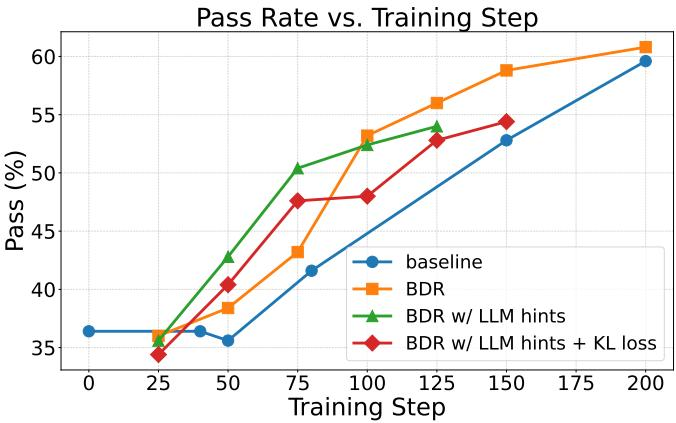
\includegraphics[keepaspectratio,alt={image}]{images/959ba60a406d67ac5148b53222aadaa90ee829eb668e27f3482dc9006bf92cc0.jpg}}

Figure 8: Ablation of Buffered Dynamic Retry under different feedback
settings.

Table 3 details the outcomes of a short-horizon BDR training regimen
initialized from the single-turn RL checkpoint. For Qwen3-8B, BDR
elevates the Pass@8 from 59.6\% to 62.4\%, successfully resurrecting
approximately 16\% of initially completely failed samples. For Qwen3-9B,
BDR advances the Pass@8 from 73.2\% to 74.4\%, yielding a recovery rate
of approximately 28\%. This underscores that BDR does not merely naively
augment the dataset volume;

it selectively resurrects actionable learning signals exclusively on
instances where the current policy genuinely fails. A higher recovery
rate directly proxies the policy's enhanced capacity to autonomously
assimilate execution feedback for self-correction.

Table 3: Effect of Buffered Dynamic Retry. The results are obtained by
continuing training from the best single-turn RL checkpoints.

{\def\LTcaptype{none} % do not increment counter
\begin{longtable}[]{@{}llll@{}}
\toprule\noalign{}
\endhead
\bottomrule\noalign{}
\endlastfoot
Model & Method & Pass@8 & Recovery Rate \\
\multirow{2}{*}{Qwen3-8B} & Baseline & 59.6\% & - \\
& BDR & 62.4\% & \textasciitilde16\% \\
\multirow{2}{*}{Qwen3.5-9B} & Baseline & 73.2\% & - \\
& BDR & 74.4\% & \textasciitilde28\% \\
\end{longtable}
}

It is crucial to note that BDR is fundamentally ill-suited as a
high-frequency global training regimen throughout the entire RL
pipeline. Because it structurally transfigures a subset of zero-shot
generation tasks into feedback-conditioned repair tasks, excessive or
premature integration risks task interference, potentially eroding the
primary objective of first-turn synthesis. Consequently, we
strategically deploy BDR strictly as a late-stage stabilization
technique. Once the model has attained a robust baseline generation
proficiency, feedback-augmented samples are introduced at a marginal
sampling ratio, serving specifically to conquer the long-tail boundary
of hard tasks.

\subsection{5.4.6 EFFECT OF MIRRORPOP}\label{effect-of-mirrorpop}

The ablation results show that MirrorPop plays an important role in both
final performance and RL training stability. As reported in Table 2,
removing MirrorPop reduces the Overall Pass@8 from 93.2\% to 86.0\% and
the Avg.@8 from 88.60\% to 80.75\%, corresponding to absolute drops of
7.2 and 7.85 percentage points, respectively. The performanceoriented
metrics also degrade: the Faster Rate vs.~Eager decreases from 15.0\% to
13.1\%, while the Faster Rate vs.~Compile drops from 9.2\% to 7.8\%.
These results indicate that MirrorPop is not merely a training-curve
smoothing heuristic; it directly contributes to final kernel correctness
and empirical speedup.

Figure 9 further compares three sequence-level off-policy masking
configurations: Null, which disables sequencelevel filtering and updates
the policy using all rollouts; Vanilla, which performs masking based on
conventional signed log-ratio aggregation; and MirrorPop, which masks
sequences according to absolute log-ratio deviations. All three runs are
continued from the same strong checkpoint, selected according to the
best validation performance before this ablation.

The training reward trajectories reveal a clear difference among the
three settings. Both Null and Vanilla suffer from an initial reward drop
after continued training begins, indicating that the policy can be
destabilized when highmismatch trajectories are not reliably filtered.
Vanilla later recovers part of the lost reward, suggesting that signed
log-ratio masking still removes some harmful off-policy samples.
However, its recovered reward remains below MirrorPop, while Null shows
little or only marginal recovery after the drop. Overall, Null and
Vanilla both degrade to a substantially lower reward level than
MirrorPop, with the main difference being that Vanilla partially
rebounds whereas Null largely fails to recover. In contrast, MirrorPop
maintains a consistently higher and more stable reward trajectory,
indicating more reliable identification and suppression of high-risk
off-policy samples.

The entropy, gradient norm, and response length clipping curves (Figure
9, b-d) provide consistent evidence. Under Null, the model shows
pronounced fluctuations in gradient norm and entropy, together with a
higher response length clipping ratio, indicating unstable optimization
and a tendency toward pathological long responses. Vanilla partially
alleviates these issues, but still exhibits noticeable oscillations.
MirrorPop produces smoother gradient dynamics, more controlled entropy,
and a lower response length clipping ratio, suggesting that its
sequence-level filtering improves both optimization stability and
output-structure control.

To further analyze off-policy behavior, we report two passive
sequence-level diagnostics corresponding to the Vanilla and MirrorPop
formulations (Figure 9, e-f). The Vanilla-form diagnostic computes the
signed mean log-ratio:
\(\begin{array} { r } { \frac { 1 } { L _ { i } } \sum _ { t = 1 } ^ { L _ { i } } \log \rho _ { i , t } } \end{array}\)
. This statistic measures the signed average shift of a response, but
positive and negative tokenlevel deviations can cancel each other. The
MirrorPop-form diagnostic instead computes the mean absolute log-ratio:
\(\begin{array} { r l } {  { \frac { 1 } { L _ { i } } \sum _ { t = 1 } ^ { L _ { i } } } } & { { } } \end{array}\)
\textbar log \(\rho _ { i , t } |\) , which measures the magnitude of
sequence-level policy mismatch regardless of direction.

The two diagnostics reveal different behaviors. Under the Vanilla-form
metric, both Null and Vanilla strategies first increase and then
decrease, without showing a clear trend of off-policy control. However,
under the MirrorPop-form metric, Null strategy continues to increase
over training, while Vanilla strategy still shows a rise-and-fall
pattern.

\pandocbounded{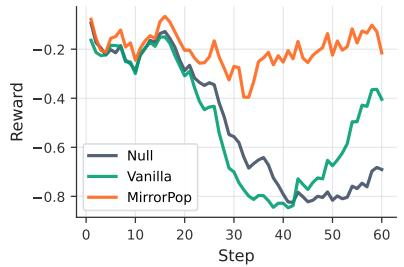
\includegraphics[keepaspectratio,alt={image}]{images/5848d37693c77433ce4cf61ada88e56673e2ad42b3f7fff9593824c07c115731.jpg}}

\begin{enumerate}
\def\labelenumi{(\alph{enumi})}
\tightlist
\item
  Training reward
\end{enumerate}

\pandocbounded{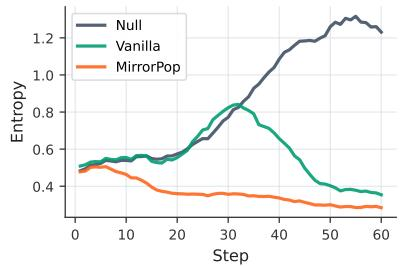
\includegraphics[keepaspectratio,alt={image}]{images/be1c97d24284cf34b6ab1fab17d82c0a8d28b58f7c15e3a6bbf02528b69537b3.jpg}}

\begin{enumerate}
\def\labelenumi{(\alph{enumi})}
\setcounter{enumi}{1}
\tightlist
\item
  Entropy
\end{enumerate}

\pandocbounded{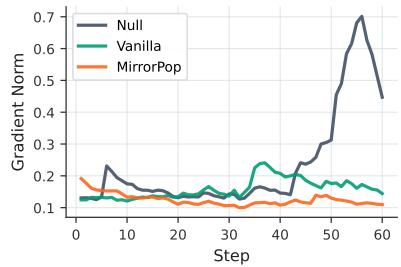
\includegraphics[keepaspectratio,alt={image}]{images/4235a15e2c74d88a2886b23b87981401b7ecfd0d3d9b0942b2bcf84b863b75cf.jpg}}

\begin{enumerate}
\def\labelenumi{(\alph{enumi})}
\setcounter{enumi}{2}
\tightlist
\item
  Gradient norm
\end{enumerate}

\pandocbounded{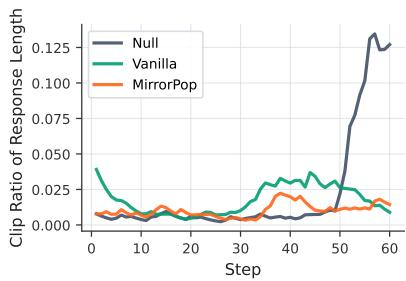
\includegraphics[keepaspectratio,alt={image}]{images/51482b81d3bcbddb099f6bc1ed18d0c68521f5f70bdf59632db10046f366643b.jpg}}

\begin{enumerate}
\def\labelenumi{(\alph{enumi})}
\setcounter{enumi}{3}
\tightlist
\item
  Response length clip ratio
\end{enumerate}

\pandocbounded{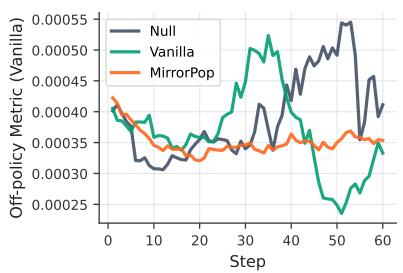
\includegraphics[keepaspectratio,alt={image}]{images/0366d23f28195136c222e3c7a949b0bc1f81ef7759bc2aaff39acc57e7d91fe9.jpg}}

\begin{enumerate}
\def\labelenumi{(\alph{enumi})}
\setcounter{enumi}{4}
\tightlist
\item
  Off-policy metric in Vanilla form
\end{enumerate}

\pandocbounded{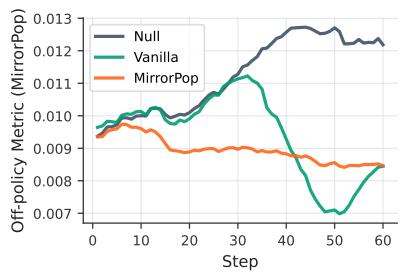
\includegraphics[keepaspectratio,alt={image}]{images/56e60c3cc68ff2080ce4791c6354671c67f3e293c4af3e48e4d399d9681978bc.jpg}}

\begin{enumerate}
\def\labelenumi{(\alph{enumi})}
\setcounter{enumi}{5}
\tightlist
\item
  Off-policy metric in MirrorPop form
\end{enumerate}

Figure 9: Training dynamics under different off-policy sequence masking
strategies: Null, Vanilla, and MirrorPop. All runs are continued from
the same checkpoint selected before this ablation. The last two panels
report passive sequence-level off-policy diagnostics computed in the
Vanilla signed-log-ratio form and the MirrorPop absolute-logratio form,
respectively.

This discrepancy suggests that signed log-ratio aggregation can
underestimate the true severity of off-policy drift due to cancellation,
and therefore may provide a misleading picture of whether high-mismatch
trajectories are being effectively controlled. In contrast, MirrorPop
strategy remains stable and gradually decreases under both diagnostics,
indicating more consistent control over sequence-level policy drift.

Overall, these results support the design rationale of MirrorPop. Rather
than measuring only the directional bias of a response relative to the
rollout policy, MirrorPop estimates the magnitude of sequence-level
mismatch. This allows it to more reliably mask severely off-policy
samples, thereby reducing unstable policy updates and improving the
stability of RL training.

\subsection{5.5 MUSA KERNELBENCH}\label{musa-kernelbench}

To further evaluate MusaCoder's cross-backend kernel generation
capability, we conduct experiments on a MUSAported variant of
KernelBench. This benchmark is adapted from the original CUDA version
while preserving the same task structure and difficulty splits. We
replace CUDA-specific task descriptions, backend constraints, and
deviceplacement operations with their MUSA counterparts, e.g., mapping
.cuda() to .musa(). For prompt exemplars that contain CUDA kernels, we
use Musify to convert CUDA APIs, launch interfaces, and compilation
commands into MUSA-compatible implementations. Converted exemplars are
further checked through compilation and correctness validation, and only
verified examples are retained to ensure consistency with the MUSA
runtime.

Since torch.compile has not yet been fully benchmarked on the current
MUSA platform, we report Faster Rate only against PyTorch eager
execution. A candidate is counted as faster only if it passes
correctness and legality checks and achieves a speedup greater than
1.1×, filtering out marginal timing noise. We compare MusaCoder with
strong general code models, including DeepSeek-V4-Pro and GLM-5.1, to
assess whether a model trained with CUDA/- MUSA kernel data and
execution feedback can generate native MUSA kernels directly from
PyTorch references.

Table 4 shows that execution-feedback training consistently improves
MusaCoder on the MUSA backend. For the 9B model, RL increases Overall
Pass@8 from 64.8\% to 84.4\%, Avg.@8 from 56.2\% to 72.3\%, and Faster
Rate from 1.9\% to 6.4\%. For the 27B model, RL further improves Overall
Pass@8 from 79.6\% to 92.4\%, Avg.@8 from 63.5\% to 81.7\%, and Faster
Rate from 5.2\% to 12.5\%. These gains indicate that RL does not merely
improve functional correctness; it also helps the model discover
implementation patterns that are more likely to accelerate on the MUSA
backend.

Table 4: MUSA KernelBench evaluation results. We report
correctness-oriented Pass Rate metrics and performanceoriented Faster
Rate metrics across Overall, Level 1, Level 2, and Level 3. Pass@8
denotes whether at least one of 8 sampled candidates passes
verification, while Avg.@8 measures the average correctness rate among 8
samples. Faster denotes Faster Rate against PyTorch eager execution;
torch.compile was not evaluated on the MUSA platform. A candidate is
counted as faster only when its speedup is larger than 1.1×.

{\def\LTcaptype{none} % do not increment counter
\begin{longtable}[]{@{}lllllllllllll@{}}
\toprule\noalign{}
\endhead
\bottomrule\noalign{}
\endlastfoot
\multirow{2}{*}{Model} & \multicolumn{3}{l}{%
Overall} & \multicolumn{3}{l}{%
Level 1} & \multicolumn{3}{l}{%
Level 2} & \multicolumn{3}{l@{}}{%
Level 3} \\
& Pass@8 & Avg.@8 & Faster & Pass@8 & Avg.@8 & Faster & Pass@8 & Avg.@8
& Faster & Pass@8 & Avg.@8 & Faster \\
DeepSeek-V4-Pro & 92.0 & 56.9 & 5.7 & 96 & 63.9 & 6.6 & 96 & 61.5 & 7.5
& 76 & 33.8 & 0.0 \\
GLM-5.1 & 88.0 & 66.4 & 6.9 & 92 & 75.5 & 8.3 & 93 & 68.1 & 8.9 & 70 &
45.0 & 0.0 \\
MusaCoder-9B-SFT & 64.8 & 56.2 & 1.9 & 84 & 74.0 & 3.1 & 68 & 59.0 & 1.7
& 20 & 15.0 & 0.0 \\
MusaCoder-9B-RL & 84.4 & 72.3 & 6.4 & 94 & 82.5 & 9.0 & 90 & 77.0 & 5.7
& 54 & 42.5 & 2.6 \\
MusaCoder-27B-SFT & 79.6 & 63.5 & 5.2 & 92 & 80.1 & 7.6 & 84 & 64.5 &
4.9 & 46 & 27.9 & 1.0 \\
MusaCoder-27B-RL & 92.4 & 81.7 & 12.5 & 98 & 92.7 & 19.6 & 96 & 84.2 &
10.0 & 74 & 54.1 & 3.3 \\
\end{longtable}
}

Compared with general-purpose code models, MusaCoder-27B-RL achieves the
strongest overall stability and performance. Although DeepSeek-V4-Pro
already reaches a high Overall Pass@8 of 92.0\%, its Avg.@8 is only
56.9\%, suggesting that correct solutions appear less consistently
across samples. MusaCoder-27B-RL achieves a similar Pass@8 of 92.4\% but
substantially higher Avg.@8 of 81.7\%, improving single-sample
correctness stability by 24.8 points. It also improves Faster Rate from
DeepSeek's 5.7\% and GLM's 6.9\% to 12.5\%. On Level 3, MusaCoder-27B-RL
reaches 54.1\% Avg.@8 and 3.3\% Faster Rate, while both baselines obtain
0.0\% Faster Rate, showing that MusaCoder is more effective at
generating usable and accelerated kernels for difficult MUSA workloads.

These results strengthen the central claim of this technical report:
MusaCoder is not only a CUDA-oriented kernel generation model, but also
a cross-backend native kernel synthesis system. The same data
construction, verification, and execution-feedback training pipeline can
transfer to the MUSA ecosystem and produce competitive native-kernel
generation capability. This provides an important foundation for
building an open MUSA kernel generation community, where LLMs can assist
developers in writing, validating, repairing, and optimizing
backend-specific GPU kernels.

\subsection{REFERENCES}\label{references}

Jason Ansel, Edward Yang, Horace He, Natalia Gimelshein, Animesh Jain,
Michael Voznesensky, Bin Bao, Peter Bell, David Berard, Evgeni Burovski,
Geeta Chauhan, Anjali Chourdia, Will Constable, Alban Desmaison, Zachary
DeVito, Elias Ellison, Will Feng, Jiong Gong, Michael Gschwind, Brian
Hirsh, Sherlock Huang, Kshiteej Kalambarkar, Laurent Kirsch, Michael
Lazos, Mario Lezcano, Yanbo Liang, Jason Liang, Yinghai Lu, C. K. Luk,
Bert Maher, Yunjie Pan, Christian Puhrsch, Matthias Reso, Mark Saroufim,
Marcos Siraichi, Helen Suk, Shunting Zhang, Michael Suo, Phil Tillet,
Eikan Wang, Xiaodong Zhou, Richard Zou, Xiaodong Wang, Ajit Mathews,
Gregory Chanan, Peng Wu, and Soumith Chintala. Pytorch 2: Faster machine
learning through dynamic python bytecode transformation and graph
compilation, 2024. URL https://pytorch.org/assets/pytorch2-2.pdf.

Haolei Bai, Lingcheng Kong, Xueyi Chen, Jianmian Wang, Zhiqiang Tao, and
Huan Wang. Dice: Diffusion large language models excel at generating
cuda kernels. arXiv preprint arXiv:2602.11715, 2026. URL https://ar
xiv.org/abs/2602.11715.

Yuntao Bai, Andy Jones, Kamal Ndousse, Amanda Askell, Anna Chen, Nova
DasSarma, Dawn Drain, Stanislav Fort, Deep Ganguli, Tom Henighan,
Nicholas Joseph, Saurav Kadavath, Jackson Kernion, Tom Conerly, Sheer
El-Showk, Nelson Elhage, Zac Hatfield-Dodds, Danny Hernandez, Tristan
Hume, Scott Johnston, Shauna Kravec, Liane Lovitt, Neel Nanda, Catherine
Olsson, Dario Amodei, Tom Brown, Jack Clark, Sam McCandlish, Chris Olah,
Ben Mann, and Jared Kaplan. Training a helpful and harmless assistant
with reinforcement learning from human feedback, 2022. URL
https://arxiv.org/abs/2204.05862.

Carlo Baronio, Pietro Marsella, Ben Pan, Simon Guo, and Silas Alberti.
Kevin: Multi-turn rl for generating cuda kernels. arXiv preprint
arXiv:2507.11948, 2025. URL https://arxiv.org/abs/2507.11948.

Matya´s Brabec, Ji ˇ ˇr´ı Klepl, Michal Topfer, and Martin Kruli ¨ s.
Tutoring llm into a better cuda optimizer. ˇ arXiv preprint
arXiv:2510.16933, 2025. URL https://arxiv.org/abs/2510.16933.

Cambricon. Bang c/c++ programming guide.
https://developer.cambricon.com/index/docume
nt/details/classid/3/cid/28/id/407.html, 2026. Official Cambricon
developer documentation, accessed 2026-05-13.

Tianqi Chen, Thierry Moreau, Ziheng Jiang, Lianmin Zheng, Eddie Qian
Yan, Haichen Shen, Jonathan Cowan, Leyuan Wang, Yuwei Hu, Luis Ceze,
Carlos Guestrin, and Arvind Krishnamurthy. Tvm: An automated end-to-end
optimizing compiler for deep learning. In 13th USENIX Symposium on
Operating Systems Design and Implementation (OSDI 18), pages 578--594.
USENIX Association, 2018. URL https://www.usenix.org/conference/
osdi18/presentation/chen.

Paul F. Christiano, Jan Leike, Tom B. Brown, Miljan Martic, Shane Legg,
and Dario Amodei. Deep reinforcement learning from human preferences. In
Advances in Neural Information Processing Systems, volume 30, 2017. URL
https://arxiv.org/abs/1706.03741.

Weinan Dai, Hanlin Wu, Qiying Yu, Huan-ang Gao, Jiahao Li, Chengquan
Jiang, Weiqiang Lou, Yufan Song, Hongli Yu, Jiaze Chen, et al.~Cuda
agent: Large-scale agentic rl for high-performance cuda kernel
generation. arXiv preprint arXiv:2602.24286, 2026. URL
https://arxiv.org/abs/2602.24286.

Yangruibo Ding, Marcus J. Min, Gail Kaiser, and Baishakhi Ray. Cycle:
Learning to self-refine the code generation. arXiv preprint
arXiv:2403.18746, 2024. URL https://arxiv.org/abs/2403.18746.

Kris Shengjun Dong, Sahil Modi, Dima Nikiforov, Sana Damani, Edward Lin,
Siva Kumar Sastry Hari, and Christos Kozyrakis. Kernelblaster: Continual
cross-task cuda optimization via memory-augmented in-context
reinforcement learning, 2026. URL https://arxiv.org/abs/2602.14293.

Dibakar Gope, David Mansell, Danny Loh, and Ian Bratt. Highly optimized
kernels and fine-grained codebooks for llm inference on arm cpus. arXiv
preprint arXiv:2501.00032, 2024.

Daya Guo, Dejian Yang, Haowei Zhang, Junxiao Song, Peiyi Wang, Qihao
Zhu, Runxin Xu, Ruoyu Zhang, Shirong Ma, et al.~Deepseek-r1 incentivizes
reasoning in llms through reinforcement learning. Nature,
645(8081):633--638, September 2025. ISSN 1476-4687. doi:
10.1038/s41586-025-09422-z. URL http://dx.doi.org/10.10
38/s41586-025-09422-z.

Siqi Guo, Ming Lin, and Tianbao Yang. Drtriton: Large-scale synthetic
data reinforcement learning for triton kernel generation, 2026. URL
https://arxiv.org/abs/2603.21465.

Pin-Lun Hsu, Yun Dai, Vignesh Kothapalli, Qingquan Song, Shao Tang, Siyu
Zhu, Steven Shimizu, Shivam Sahni, Haowen Ning, and Yanning Chen. Liger
kernel: Efficient triton kernels for llm training. arXiv preprint
arXiv:2410.10989, 2024. URL https://arxiv.org/abs/2410.10989.

Huawei. Cann documentation.
https://www.hiascend.com/document/detail/zh/canncommer
cial/80RC3/overview/index.html, 2026. Official Huawei Ascend CANN
documentation, accessed 2026-05-13.

Jaber Jaber and Osama Jaber. Autokernel: Autonomous gpu kernel
optimization via iterative agent-driven search, 2026. URL
https://arxiv.org/abs/2603.21331.

Shangzhan Li, Zefan Wang, Ye He, Yuxuan Li, Qi Shi, Jianling Li,
Yonggang Hu, Wanxiang Che, Xu Han, Zhiyuan Liu, and Maosong Sun.
Autotriton: Automatic triton programming with reinforcement learning in
llms. CoRR, abs/2507.05687, July 2025a. URL
https://doi.org/10.48550/arXiv.2507.05687.

Xiaoya Li, Xiaofei Sun, Albert Wang, Jiwei Li, and Chris Shum. Cuda-l1:
Improving cuda optimization via contrastive reinforcement learning.
arXiv preprint arXiv:2507.14111, 2025b. URL https://arxiv.org/abs/2507.1
4111.

Yingru Li, Jiacai Liu, Jiawei Xu, Yuxuan Tong, Ziniu Li, Qian Liu, and
Baoxiang Wang. Trust region masking for long-horizon llm reinforcement
learning, 2026. URL https://arxiv.org/abs/2512.23075.

Aixin Liu, Aoxue Mei, Bangcai Lin, Bing Xue, Bingxuan Wang, Bingzheng
Xu, Bochao Wu, Bowei Zhang, Chaofan Lin, Chen Dong, et
al.~Deepseek-v3.2: Pushing the frontier of open large language models.
arXiv preprint arXiv:2512.02556, 2025a.

Jiacai Liu, Yingru Li, Yuqian Fu, Jiawei Wang, Qian Liu, and Zhuo Jiang.
When speed kills stability: Demystifying RL collapse from the
training-inference mismatch, September 2025b. URL
https://richardli.xyz/rl-c ollapse.

Jiawei Liu, Jinkun Lin, Fabian Ruffy, Cheng Tan, Jinyang Li, Aurojit
Panda, and Lingming Zhang. Nnsmith: Generating diverse and valid test
cases for deep learning compilers. In Proceedings of the 28th ACM
International Conference on Architectural Support for Programming
Languages and Operating Systems, Volume 2, pages 530-- 543, 2023.

Ilya Loshchilov and Frank Hutter. Decoupled weight decay regularization.
arXiv preprint arXiv:1711.05101, 2017.

Aman Madaan, Niket Tandon, Prakhar Gupta, Skyler Hallinan, Luyu Gao,
Sarah Wiegreffe, Uri Alon, Nouha Dziri, Shrimai Prabhumoye, Yiming Yang,
Shashank Gupta, Bodhisattwa Prasad Majumder, Katherine Hermann, Sean
Welleck, Amir Yazdanbakhsh, and Peter Clark. Self-refine: Iterative
refinement with self-feedback. arXiv preprint arXiv:2303.17651, 2023.
URL https://arxiv.org/abs/2303.17651.

Moore Threads. Musa sdk documentation.
https://docs.mthreads.com/musa-sdk/musa-sdk-doc-o nline/introduction/,
2026. Official Moore Threads MUSA SDK documentation, accessed
2026-05-13.

NVIDIA. Cuda c++ programming guide.
https://docs.nvidia.com/cuda/cuda-c-programming-g uide/, 2026a. Accessed
2026-05-20.

NVIDIA. Nvidia nsight compute documentation.
https://docs.nvidia.com/nsight-compute/, 2026b. Accessed 2026-05-20.

NVIDIA. Nvidia nsight systems documentation.
https://docs.nvidia.com/nsight-systems/, 2026c. Accessed 2026-05-20.

Anne Ouyang, Simon Guo, Simran Arora, Alex L Zhang, William Hu,
Christopher Re, and Azalia Mirhoseini. Ker-´ nelbench: Can llms write
efficient gpu kernels? arXiv preprint arXiv:2502.10517, 2025.

Long Ouyang, Jeff Wu, Xu Jiang, Diogo Almeida, Carroll L. Wainwright,
Pamela Mishkin, Chong Zhang, Sandhini Agarwal, Katarina Slama, Alex Ray,
John Schulman, Jacob Hilton, Fraser Kelton, Luke Miller, Maddie Simens,
Amanda Askell, Peter Welinder, Paul Christiano, Jan Leike, and Ryan
Lowe. Training language models to follow instructions with human
feedback. In Proceedings of the Conference on Neural Information
Processing Systems (NeurIPS 2022), 2022.

Adam Paszke, Sam Gross, Francisco Massa, Adam Lerer, James Bradbury,
Gregory Chanan, Trevor Killeen, Zeming Lin, Natalia Gimelshein, Luca
Antiga, Alban Desmaison, Andreas Kopf, Edward Yang, Zachary DeVito,
Martin Raison, Alykhan Tejani, Sasank Chilamkurthy, Benoit Steiner, Lu
Fang, Junjie Bai, and Soumith Chintala. Pytorch: An imperative style,
high-performance deep learning library. In Advances in Neural
Information Processing Systems, volume 32, 2019. URL
https://arxiv.org/abs/1912.01703.

Samyam Rajbhandari, Jeff Rasley, Olatunji Ruwase, and Yuxiong He. Zero:
Memory optimizations toward training trillion parameter models. In SC20:
international conference for high performance computing, networking,
storage and analysis, pages 1--16. IEEE, 2020.

James Reed, Zachary DeVito, Horace He, Ansley Ussery, and Jason Ansel.
Torch.fx: Practical program capture and transformation for deep learning
in python. In Proceedings of Machine Learning and Systems, volume 4,
pages 638--651, 2022. URL https://arxiv.org/abs/2112.08429.

John Schulman, Filip Wolski, Prafulla Dhariwal, Alec Radford, and Oleg
Klimov. Proximal policy optimization algorithms, 2017. URL
https://arxiv.org/abs/1707.06347.

Zhihong Shao, Peiyi Wang, Qihao Zhu, Runxin Xu, Junxiao Song, Xiao Bi,
Haowei Zhang, Mingchuan Zhang, YK Li, Yang Wu, et al.~Deepseekmath:
Pushing the limits of mathematical reasoning in open language models.
arXiv preprint arXiv:2402.03300, 2024.

Noah Shinn, Federico Cassano, Edward Berman, Ashwin Gopinath, Karthik
Narasimhan, and Shunyu Yao. Reflexion: Language agents with verbal
reinforcement learning. arXiv preprint arXiv:2303.11366, 2023. URL
https: //arxiv.org/abs/2303.11366.

Mohammad Shoeybi, Mostofa Patwary, Raul Puri, Patrick LeGresley, Jared
Casper, and Bryan Catanzaro. Megatronlm: Training multi-billion
parameter language models using model parallelism. arXiv preprint
arXiv:1909.08053, 2019.

Nisan Stiennon, Long Ouyang, Jeffrey Wu, Daniel Ziegler, Ryan Lowe,
Chelsea Voss, Alec Radford, Dario Amodei, and Paul F Christiano.
Learning to summarize with human feedback. In Proceedings of the
Advances in Neural Information Processing Systems (NeurIPS'20), 2020.

Philippe Tillet, Hsiang-Tsung Kung, and David Cox. Triton: An
intermediate language and compiler for tiled neural network
computations. In Proceedings of the 3rd ACM SIGPLAN International
Workshop on Machine Learning and Programming Languages, pages 10--19,
2019. doi: 10.1145/3315508.3329973.

Han Wang, Jintao Zhang, Kai Jiang, Haoxu Wang, Jianfei Chen, and Jun
Zhu. Kernelbenchx: A comprehensive benchmark for evaluating
llm-generated gpu kernels. arXiv preprint arXiv:2605.04956, 2026. URL
https: //arxiv.org/abs/2605.04956.

Xingyao Wang, Boxuan Li, Yufan Song, Frank F. Xu, Xiangru Tang, Mingchen
Zhuge, Jiayi Pan, Yueqi Song, Bowen Li, Jaskirat Singh, Hoang H. Tran,
Fuqiang Li, Ren Ma, Mingzhang Zheng, Bill Qian, Yanjun Shao, Niklas
Muennighoff, Yizhe Zhang, Binyuan Hui, Junyang Lin, Robert Brennan, Hao
Peng, Heng Ji, and Graham Neubig. Openhands: An open platform for ai
software developers as generalist agents. arXiv preprint
arXiv:2407.16741, 2024. URL https://arxiv.org/abs/2407.16741.

Yinjie Wang, Ling Yang, Ye Tian, Ke Shen, and Mengdi Wang. Co-evolving
llm coder and unit tester via reinforcement learning. arXiv preprint
arXiv:2506.03136, 2025. URL https://arxiv.org/abs/2506.03136.

An Yang, Anfeng Li, Baosong Yang, Beichen Zhang, Binyuan Hui, Bo Zheng,
Bowen Yu, Chang Gao, Chengen Huang, Chenxu Lv, Chujie Zheng, Dayiheng
Liu, Fan Zhou, Fei Huang, Feng Hu, Hao Ge, Haoran Wei, Huan Lin, Jialong
Tang, Jian Yang, Jianhong Tu, Jianwei Zhang, Jianxin Yang, Jiaxi Yang,
Jing Zhou, Jingren Zhou, Junyang Lin, Kai Dang, Keqin Bao, Kexin Yang,
Le Yu, Lianghao Deng, Mei Li, Mingfeng Xue, Mingze Li, Pei Zhang, Peng
Wang, Qin Zhu, Rui Men, Ruize Gao, Shixuan Liu, Shuang Luo, Tianhao Li,
Tianyi Tang, Wenbiao Yin,

Xingzhang Ren, Xinyu Wang, Xinyu Zhang, Xuancheng Ren, Yang Fan, Yang
Su, Yichang Zhang, Yinger Zhang, Yu Wan, Yuqiong Liu, Zekun Wang, Zeyu
Cui, Zhenru Zhang, Zhipeng Zhou, and Zihan Qiu. Qwen3 technical report,
2025. URL https://arxiv.org/abs/2505.09388.

John Yang, Carlos E. Jimenez, Alexander Wettig, Kilian Lieret, Shunyu
Yao, Karthik Narasimhan, and Ofir Press. Swe-agent: Agent-computer
interfaces enable automated software engineering. arXiv preprint
arXiv:2405.15793, 2024. URL https://arxiv.org/abs/2405.15793.

Feng Yao, Liyuan Liu, Dinghuai Zhang, Chengyu Dong, Jingbo Shang, and
Jianfeng Gao. Your efficient rl framework secretly brings you off-policy
rl training, August 2025. URL https://fengyao.notion.site/off-pol
icy-rl.

Yufan Ye, Ting Zhang, Wenbin Jiang, and Hua Huang. Process-supervised
reinforcement learning for code generation. arXiv preprint
arXiv:2502.01715, 2025. URL https://arxiv.org/abs/2502.01715.

Zijian Zhang, Rong Wang, Shiyang Li, Yuebo Luo, Mingyi Hong, and Caiwen
Ding. Cudaforge: An agent framework with hardware feedback for cuda
kernel optimization. arXiv preprint arXiv:2511.01884, 2025. URL https:
//arxiv.org/abs/2511.01884.

Xin Zhao, Yongkang Liu, Kuan Xu, Jia Guo, Zihao Wang, Yan Sun, Xinyu
Kong, Qianggang Cao, Liang Jiang, Zujie Wen, Zhiqiang Zhang, and Jun
Zhou. Small leak can sink a great ship--boost rl training on moe with
icepop!, Sep 2025. URL https://ringtech.notion.site/icepop.

Lianmin Zheng, Chengfan Jia, Minmin Sun, Zhao Wu, Cody Hao Yu, Ameer
Haj-Ali, Yida Wang, Jun Yang, Danyang Zhuo, Koushik Sen, Joseph E.
Gonzalez, and Ion Stoica. Ansor: Generating high-performance tensor
programs for deep learning. In 14th USENIX Symposium on Operating
Systems Design and Implementation (OSDI 20), pages 863--879. USENIX
Association, 2020. URL https://www.usenix.org/conference/osdi20/prese
ntation/zheng.

Lianmin Zheng, Liangsheng Yin, Zhiqiang Xie, Chuyue Huang, Jeff Sun,
Cody Hao Yu, Shiyi Cao, Christos Kozyrakis, Ion Stoica, Joseph E.
Gonzalez, Clark Barrett, and Ying Sheng. Sglang: Efficient execution of
structured language model programs. In Advances in Neural Information
Processing Systems, 2024. URL https://arxiv.org/abs/2312.07104.

Xinguo Zhu, Shaohui Peng, Jiaming Guo, Yunji Chen, Qi Guo, Yuanbo Wen,
Hang Qin, Ruizhi Chen, Qirui Zhou, Ke Gao, Yanjun Wu, Chen Zhao, and
Ling Li. Qimeng-kernel: Macro-thinking micro-coding paradigm for
llmbased high-performance gpu kernel generation. arXiv preprint
arXiv:2511.20100, 2025. URL https://arxi v.org/abs/2511.20100.

\subsection{A REVISED PROMPT FOR
KERNELBENCH}\label{a-revised-prompt-for-kernelbench}

\begin{Shaded}
\begin{Highlighting}[]
\NormalTok{You are an expert Performance Engineer specializing in CUDA and PyTorch internals.}

\NormalTok{\#\#\# STRICT MANDATE: TOTAL CONVERSION}
\NormalTok{You must optimize the provided architecture, named \textasciigrave{}Model\textasciigrave{}, by replacing standard PyTorch operator with a custom CUDA kernel.}
\NormalTok{1. **No Standard Ops:** You are STRICTLY FORBIDDEN from using standard PyTorch compute functions (e.g., \textasciigrave{}torch.matmul\textasciigrave{}, \textasciigrave{}torch.relu\textasciigrave{}) in the forward pass.}
\NormalTok{2. **Fusion:** You may fuse consecutive operators (e.g., merging MatMul + Bias + Activation) to minimize memory access.}
\NormalTok{3. **Scope of Work:** Focus ONLY on the nn.Module class definition. Ignore any other codes, for example codes that are related to testing.}

\NormalTok{\#\#\# CRITICAL: WEIGHTS VS COMPUTATION}
\NormalTok{The optimized \textasciigrave{}ModelNew\textasciigrave{} will load pre{-}trained weights from the original \textasciigrave{}Model\textasciigrave{} when testing, but you MUST NOT use the original PyTorch implementations for compute.}

\NormalTok{**1. Rules for \textasciigrave{}init\textasciigrave{} (Preserve Structure):**}
\NormalTok{You MUST preserve the original \textasciigrave{}nn.Module\textasciigrave{} definitions (e.g., \textasciigrave{}self.conv = nn.Conv2d(...)\textasciigrave{}). This is required solely to ensure variable names and shapes match the original \textasciigrave{}state\_dict\textasciigrave{} for loading weights.}

\NormalTok{**2. Rules for \textasciigrave{}forward\textasciigrave{} (Custom Compute):**}
\NormalTok{You are **STRICTLY FORBIDDEN** from calling the module objects directly. You must access their underlying parameters and pass them to your custom kernels.}
\NormalTok{E.g.,}
\NormalTok{* **FORBIDDEN:** \textasciigrave{}out = self.conv(x)\textasciigrave{} or \textasciigrave{}out = self.fc(x)\textasciigrave{} }
\NormalTok{* **REQUIRED:** \textasciigrave{}out = custom\_kernel(x, self.conv.weight, self.conv.bias)\textasciigrave{} }

\NormalTok{\#\#\# Reference Examples (This is only for one{-}shot example guideline. Not the real model you need to optimize.)}
\NormalTok{Here are examples of how to replace PyTorch operators with \{\{backend\_display\}\}}
\NormalTok{while maintaining state dict compatibility:}
\NormalTok{\{\{one\_shot\_example]]}

\NormalTok{\#\#\# Input Architecture (This is the actual model you need to optimize.)}
\NormalTok{Optimize the following PyTorch model definition:}
\NormalTok{\textasciigrave{}\textasciigrave{}\textasciigrave{}python}
\NormalTok{\{\{reference\_pytorch\_code]]}

\NormalTok{...}

\NormalTok{\#\#\# Output Requirements}
\NormalTok{* **Target:** Name the optimized output architecture \textasciigrave{}ModelNew‘.}
\NormalTok{* **Quality:** Generate REAL, compilable code. NOT pseudocode. Include all necessary dependencies and helper functions.}
\NormalTok{* **Formatting:** Output ONLY the code block. Do not include testing code, training loops, or conversational text.}
\NormalTok{* **load\_inline() arguments**: Leave the parameters extra\_cflags, extra\_ldflags args empty. Only include necessary args like name, cpp\_sources, cuda\_sources, functions and set verbose=False. }
\end{Highlighting}
\end{Shaded}

\subsection{B EXAMPLE OF SIX-STEP SFT
DATA}\label{b-example-of-six-step-sft-data}

This example shows how a training sample decomposes kernel generation
into semantic analysis, scalar math, shape calculus, indexing, boundary
handling, and error pre-analysis before presenting the final CUDA
implementation.

sft\_data\_enhanced = \{ '\,`'instruction'`:'`'Please perform an
in-depth operator translation from PyTorch to a CUDA Kernel. You must
include an exhaustive derivation of the mathematics, shape
transformations, and index mappings.'',
'\,`'input\_pytorch\_code'`:'\,'\,'\,```` import torch import torch.nn
as nn

class Model(nn.Module): def \textbf{init}(self, num\_groups,
num\_channels, eps=1e-5): super(Model, self).\_\_init\_\_()
self.num\_groups = num\_groups self.eps = eps self.weight =
nn.Parameter(torch.randn(num\_channels)) self.bias =
nn.Parameter(torch.randn(num\_channels))

\begin{verbatim}
def forward(self, x):
return torch.nn.functional.group_norm(x, self.num_groups, self.weight, self.bias, self.eps)
'''````
'''analysis_and_derivation'': '''````
\end{verbatim}

\subsubsection{1. Global Analysis and Operator
Decomposition}\label{global-analysis-and-operator-decomposition}

This operator is GroupNorm. Its core logic involves partitioning the
channel dimension \(C\) into \(G\) groups, and performing independent
normalization within each group (encompassing \(C/G\) channels and all
spatial pixels). * \textbf{Computational Flow}: Input \(x \rightarrow\)
Grouping \(rightarrow\) Intra-group Mean \(mu\) \(rightarrow\)
Intra-group Variance \(sigma^2\) \(rightarrow\) Standardization
\(rightarrow\) Channel-wise Affine Transformation ( \(gamma\) , \(beta\)
). * \textbf{Parameter Binding}:\\
* \texttt{x}:
\texttt{(N,\ C,\ H,\ W)\textbackslash{}\textquotesingle{}.\ *}weight\texttt{(\ \$gamma\$\ ):\ \textquotesingle{}(C,)\textquotesingle{}.\ \textbackslash{}\ *}bias\texttt{(\ \$beta\$\ ):\ \textquotesingle{}(C,)\textquotesingle{}.\ \textbackslash{}\ *}num\_groups`
( \(G\) ): Scalar.

\subsubsection{2. Atomic Mathematical
Derivation}\label{atomic-mathematical-derivation}

To facilitate parallelization, we decompose the algorithm into
accumulable forms: 1. \textbf{Statistic Accumulation}:\\
* Total elements per group: \(L = (C/G) \times H \times W\) . * First
moment (Sum): \(S_1 = \sum_{i \in \text{Group}}\) x\_i(. * Second moment
(Square Sum): \(S_2 = \sum_{i \in \text{Group}}\) x\_i\^{}2).

\begin{enumerate}
\def\labelenumi{\arabic{enumi}.}
\setcounter{enumi}{1}
\tightlist
\item
  \textbf{Moment-derived Statistics}:\\
\end{enumerate}

\begin{itemize}
\tightlist
\item
  Mean: \(mu = S_1 / L\) .
\item
  Variance: \(sigma^2 = (S_2 / L) - \mu^2\) .
\end{itemize}

\begin{enumerate}
\def\labelenumi{\arabic{enumi}.}
\setcounter{enumi}{2}
\tightlist
\item
  \textbf{Standardization Transformation}:\\
\end{enumerate}

\begin{itemize}
\tightlist
\item
  \(hat{x}_i = (x_i - \mu) \cdot \frac{1}{\sqrt{\sigma^2 + \epsilon}}\)
  .
\end{itemize}

\begin{enumerate}
\def\labelenumi{\arabic{enumi}.}
\setcounter{enumi}{3}
\tightlist
\item
  \textbf{Affine Transformation}:\\
\end{enumerate}

\begin{itemize}
\tightlist
\item
  \(y_i = \hat{x}_i \cdot \cdot \cdot \cdot \cdot \cdot \cdot \cdot \cdot \cdot \cdot \cdot \cdot \cdot \cdot \cdot \cdot \cdot \cdot \cdot \cdot \cdot \cdot \cdot \cdot \cdot \cdot \cdot \cdot \cdot \cdot \cdot \cdot \cdot \cdot \cdot \cdot \cdot \cdot \cdot \cdot \cdot \cdot \cdot \cdot \cdot \cdot \cdot \cdot \cdot\)
\end{itemize}

\begin{Shaded}
\begin{Highlighting}[]
\OperatorTok{*}\NormalTok{ For each instance \textbackslash{}}\OperatorTok{(}\NormalTok{n \textbackslash{}in }\OperatorTok{[}\DecValTok{0}\OperatorTok{,}\NormalTok{ N}\OperatorTok{{-}}\DecValTok{1}\OperatorTok{]}\NormalTok{\textbackslash{}}\OperatorTok{)}\NormalTok{ and group \textbackslash{}}\OperatorTok{(}\NormalTok{g \textbackslash{}in }\OperatorTok{[}\DecValTok{0}\OperatorTok{,}\NormalTok{ G}\OperatorTok{{-}}\DecValTok{1}\OperatorTok{]}\NormalTok{\textbackslash{}}\OperatorTok{),}\NormalTok{ summation is performed across three contiguous logical dimensions \textbackslash{}}\OperatorTok{(}\NormalTok{C}\CommentTok{//G, H, W\textbackslash{})\textbackslash{}).}
\OperatorTok{**}\NormalTok{Output Alignment}\OperatorTok{**:}\NormalTok{ The final output is restored to \textbackslash{}}\OperatorTok{(}\NormalTok{N}\OperatorTok{,}\NormalTok{ C}\OperatorTok{,}\NormalTok{ H}\OperatorTok{,}\NormalTok{ W\textbackslash{}}\OperatorTok{)}\NormalTok{\textbackslash{}}\OperatorTok{),}\NormalTok{ fully aligning its spatial structure with the input}\OperatorTok{.}

\PreprocessorTok{\#}\ErrorTok{\#\# 4. Deep Index Relational Mapping (Indexing Matrix)}
\NormalTok{Assuming the output coordinates are \textbackslash{}}\OperatorTok{(}\NormalTok{n}\OperatorTok{,}\NormalTok{ c}\OperatorTok{,}\NormalTok{ h}\OperatorTok{,}\NormalTok{ w\textbackslash{}}\OperatorTok{)}\NormalTok{\textbackslash{}}\OperatorTok{),}\NormalTok{ we must locate its corresponding group and associated statistics}\OperatorTok{:}
\FloatTok{1.} \OperatorTok{**}\NormalTok{Global Linear Index Parsing}\OperatorTok{**:} \OperatorTok{*}
\NormalTok{    \textasciigrave{}idx }\OperatorTok{=}\NormalTok{ n }\OperatorTok{*} \OperatorTok{(}\NormalTok{C}\OperatorTok{*}\NormalTok{H}\OperatorTok{*}\NormalTok{W}\OperatorTok{)} \OperatorTok{+}\NormalTok{ c }\OperatorTok{*} \OperatorTok{(}\NormalTok{H}\OperatorTok{*}\NormalTok{W}\OperatorTok{)} \OperatorTok{+}\NormalTok{ h }\OperatorTok{*}\NormalTok{ W }\OperatorTok{+}\NormalTok{ w\textbackslash{}}\OperatorTok{).}

\FloatTok{2.} \OperatorTok{**}\NormalTok{Logical Group Mapping}\OperatorTok{**:} \OperatorTok{*}
    \OperatorTok{*}\NormalTok{ Group index \textbackslash{}}\OperatorTok{(}\NormalTok{g }\OperatorTok{=}\NormalTok{ c }\CommentTok{// (C/G)\textbackslash{}).}

    \OperatorTok{*}\NormalTok{ Intra}\OperatorTok{{-}}\NormalTok{batch group offset}\OperatorTok{:}\NormalTok{ \textasciigrave{}group\_idx\_within\_batch }\OperatorTok{=}\NormalTok{ n }\OperatorTok{*}\NormalTok{ G }\OperatorTok{+}\NormalTok{ g\textbackslash{}}\OperatorTok{).}

\FloatTok{3.} \OperatorTok{**}\NormalTok{Memory Access Layout }\OperatorTok{(}\NormalTok{NCHW}\OperatorTok{)**:}
    \OperatorTok{*}\NormalTok{ \textasciigrave{}input}\OperatorTok{[}\NormalTok{idx}\OperatorTok{]}\NormalTok{\textasciigrave{} points to the element currently being processed}\OperatorTok{.}
    \OperatorTok{*}\NormalTok{ \textasciigrave{}weight}\OperatorTok{[}\NormalTok{c}\OperatorTok{]}\NormalTok{\textasciigrave{} and \textasciigrave{}bias}\OperatorTok{[}\NormalTok{c}\OperatorTok{]}\NormalTok{\textasciigrave{} point to the scaling weights corresponding to the current channel}\OperatorTok{.}

\FloatTok{4.} \OperatorTok{**}\NormalTok{Intra}\OperatorTok{{-}}\NormalTok{group Iterative Addressing }\OperatorTok{(}\ControlFlowTok{for}\NormalTok{ Mean}\OperatorTok{/}\NormalTok{Variance Computation}\OperatorTok{)**:}
    \OperatorTok{*}\NormalTok{ Iterate over \textbackslash{}}\OperatorTok{(}\NormalTok{ic \textbackslash{}in }\OperatorTok{[}\DecValTok{0}\OperatorTok{,} \OperatorTok{(}\NormalTok{C}\OperatorTok{/}\NormalTok{G}\OperatorTok{){-}}\DecValTok{1}\OperatorTok{],}\NormalTok{ ih \textbackslash{}in }\OperatorTok{[}\DecValTok{0}\OperatorTok{,}\NormalTok{ H}\OperatorTok{{-}}\DecValTok{1}\OperatorTok{],}\NormalTok{ iw \textbackslash{}in }\OperatorTok{[}\DecValTok{0}\OperatorTok{,}\NormalTok{ W}\OperatorTok{{-}}\DecValTok{1}\OperatorTok{]}\NormalTok{\textbackslash{}}\OperatorTok{)}\NormalTok{\textbackslash{}}\OperatorTok{(.}\NormalTok{\textbackslash{}}\OperatorTok{)}
    \OperatorTok{*}\NormalTok{ \textasciigrave{}offset }\OperatorTok{=} \OperatorTok{((}\NormalTok{n }\OperatorTok{*}\NormalTok{ C}\OperatorTok{)} \OperatorTok{+} \OperatorTok{(}\NormalTok{g }\OperatorTok{*} \OperatorTok{(}\NormalTok{C}\OperatorTok{/}\NormalTok{G}\OperatorTok{)} \OperatorTok{+}\NormalTok{ ic}\OperatorTok{))} \OperatorTok{*} \OperatorTok{(}\NormalTok{H }\OperatorTok{*}\NormalTok{ W}\OperatorTok{)} \OperatorTok{+}\NormalTok{ ih }\OperatorTok{*}\NormalTok{ W }\OperatorTok{+}\NormalTok{ iw\textbackslash{}}\OperatorTok{).}

\PreprocessorTok{\#}\ErrorTok{\#\# 5. Boundary Handling and Type Safety}
\OperatorTok{**}\NormalTok{Grid Out}\OperatorTok{{-}}\NormalTok{of}\OperatorTok{{-}}\NormalTok{Bounds}\OperatorTok{**:}\NormalTok{ \textasciigrave{}if }\OperatorTok{(}\NormalTok{idx }\OperatorTok{\textgreater{}=}\NormalTok{ N }\OperatorTok{*}\NormalTok{ C }\OperatorTok{*}\NormalTok{ H }\OperatorTok{*}\NormalTok{ W}\OperatorTok{)} \ControlFlowTok{return}\OperatorTok{;}\NormalTok{\textasciigrave{} Prevents trailing threads from accessing illegal memory addresses}\OperatorTok{.}
\OperatorTok{**}\NormalTok{Spatial Overflow}\OperatorTok{**:}\NormalTok{ When processing \textbackslash{}}\OperatorTok{(}\NormalTok{H}\OperatorTok{,}\NormalTok{ W\textbackslash{}}\OperatorTok{),}\NormalTok{ ensure proper multiplication order to prevent \textasciigrave{}int32\textasciigrave{} overflow }\OperatorTok{(}\NormalTok{using \textasciigrave{}long long\textasciigrave{} or \textasciigrave{}size\_t\textasciigrave{} }\ControlFlowTok{for}\NormalTok{ total calculations is recommended}\OperatorTok{).}
\OperatorTok{**}\NormalTok{Numerical Stability}\OperatorTok{**:}\NormalTok{ \textbackslash{}}\OperatorTok{(}\NormalTok{epsilon\textbackslash{}}\OperatorTok{)}\NormalTok{ must be added inside the \textasciigrave{}sqrt\textasciigrave{}}\OperatorTok{,}\NormalTok{ and }\ControlFlowTok{if}\NormalTok{ \textbackslash{}}\OperatorTok{(}\NormalTok{sigma}\OperatorTok{\^{}}\DecValTok{2}\NormalTok{\textbackslash{}}\OperatorTok{)}\NormalTok{ results in a minuscule negative value due to floating}\OperatorTok{{-}}\NormalTok{point inaccuracies}\OperatorTok{,}\NormalTok{ it must be clamped to }\DecValTok{0}\NormalTok{ using \textasciigrave{}max\textbackslash{}}\OperatorTok{).}

\PreprocessorTok{\#}\ErrorTok{\#\# 6. Error Anticipation and Pitfall Avoidance}
\OperatorTok{**}\NormalTok{Parameter Fallacies}\OperatorTok{**:}\NormalTok{ Channel dimensions must never be hardcoded}\OperatorTok{.}\NormalTok{ For instance}\OperatorTok{,}\NormalTok{ fixing \textasciigrave{}out\_channels\textasciigrave{} to }\DecValTok{16}\NormalTok{ in Case }\DecValTok{0}\NormalTok{ is a critical error}\OperatorTok{.}
\OperatorTok{**}\NormalTok{Logical Omissions}\OperatorTok{**:}\NormalTok{ The multiply}\OperatorTok{{-}}\NormalTok{add operation }\ControlFlowTok{for}\NormalTok{ weight \textbackslash{}}\OperatorTok{(}\NormalTok{gamma\textbackslash{}}\OperatorTok{)}\NormalTok{ and bias \textbackslash{}}\OperatorTok{(}\NormalTok{beta\textbackslash{}}\OperatorTok{)}\NormalTok{ must be implemented}\OperatorTok{;}\NormalTok{ Dummy implementations }\OperatorTok{(}\NormalTok{like the }\FloatTok{0.01}\BuiltInTok{f}\NormalTok{ padding in Case }\DecValTok{2}\OperatorTok{)}\NormalTok{ are strictly prohibited}\OperatorTok{.}
\OperatorTok{**}\NormalTok{Performance Bottlenecks}\OperatorTok{**:}\NormalTok{ Iterating over group elements using triple}\OperatorTok{{-}}\NormalTok{nested loops within a single thread is highly inefficient}\OperatorTok{.}\NormalTok{ It is recommended to introduce Shared Memory reduction in advanced SFT stages}\OperatorTok{.}
\NormalTok{\textasciigrave{}\textasciigrave{}\textasciigrave{}}\CharTok{\textquotesingle{}}
\NormalTok{\textasciigrave{}\textasciigrave{}\textasciigrave{}}\CharTok{\textquotesingle{}}
\NormalTok{\textasciigrave{}\textasciigrave{}output\_cuda\_kernel}\CharTok{\textquotesingle{}:}\ErrorTok{ r\textasciigrave{}\textasciigrave{}\textasciigrave{}}\CharTok{\textquotesingle{}}
\PreprocessorTok{\#include }\ImportTok{\textless{}torch/extension.h\textgreater{}}
\PreprocessorTok{\#include }\ImportTok{\textless{}cuda\_runtime.h\textgreater{}}
\PreprocessorTok{\#include }\ImportTok{\textless{}cmath\textgreater{}}

\NormalTok{\_\_global\_\_ }\DataTypeTok{void}\NormalTok{ group\_norm\_kernel\_detailed}\OperatorTok{(}
    \DataTypeTok{const} \DataTypeTok{float}\OperatorTok{*}\NormalTok{ \_\_restrict\_\_ input}\OperatorTok{,}
    \DataTypeTok{const} \DataTypeTok{float}\OperatorTok{*}\NormalTok{ \_\_restrict\_\_ weight}\OperatorTok{,}
    \DataTypeTok{const} \DataTypeTok{float}\OperatorTok{*}\NormalTok{ \_\_restrict\_\_ bias}\OperatorTok{,}
    \DataTypeTok{float}\OperatorTok{*}\NormalTok{ output}\OperatorTok{,}
    \DataTypeTok{int}\NormalTok{ N}\OperatorTok{,} \DataTypeTok{int}\NormalTok{ C}\OperatorTok{,} \DataTypeTok{int}\NormalTok{ H}\OperatorTok{,} \DataTypeTok{int}\NormalTok{ W}\OperatorTok{,} \DataTypeTok{int}\NormalTok{ G}\OperatorTok{,} \DataTypeTok{float}\NormalTok{ eps}\OperatorTok{)} \OperatorTok{\{}

    \DataTypeTok{int}\NormalTok{ idx }\OperatorTok{=}\NormalTok{ blockIdx}\OperatorTok{.}\NormalTok{x }\OperatorTok{*}\NormalTok{ blockDim}\OperatorTok{.}\NormalTok{x }\OperatorTok{+}\NormalTok{ threadIdx}\OperatorTok{.}\NormalTok{x}\OperatorTok{;}
    \DataTypeTok{int}\NormalTok{ total\_elements }\OperatorTok{=}\NormalTok{ N }\OperatorTok{*}\NormalTok{ C }\OperatorTok{*}\NormalTok{ H }\OperatorTok{*}\NormalTok{ W}\OperatorTok{;}
    \ControlFlowTok{if} \OperatorTok{(}\NormalTok{idx }\OperatorTok{\textgreater{}=}\NormalTok{ total\_elements}\OperatorTok{)} \ControlFlowTok{return}\OperatorTok{;}

    \CommentTok{// 1. Reverse Coordinate Parsing}
    \DataTypeTok{int}\NormalTok{ w }\OperatorTok{=}\NormalTok{ idx }\OperatorTok{\%}\NormalTok{ W}\OperatorTok{;}
    \DataTypeTok{int}\NormalTok{ h }\OperatorTok{=} \OperatorTok{(}\NormalTok{idx }\OperatorTok{/}\NormalTok{ W}\OperatorTok{)} \OperatorTok{\%}\NormalTok{ H}\OperatorTok{;}
    \DataTypeTok{int}\NormalTok{ c }\OperatorTok{=} \OperatorTok{(}\NormalTok{idx }\OperatorTok{/} \OperatorTok{(}\NormalTok{W }\OperatorTok{*}\NormalTok{ H}\OperatorTok{))} \OperatorTok{\%}\NormalTok{ C}\OperatorTok{;}
    \DataTypeTok{int}\NormalTok{ n }\OperatorTok{=}\NormalTok{ idx }\OperatorTok{/} \OperatorTok{(}\NormalTok{W }\OperatorTok{*}\NormalTok{ H }\OperatorTok{*}\NormalTok{ C}\OperatorTok{);} 
\end{Highlighting}
\end{Shaded}

\begin{Shaded}
\begin{Highlighting}[]
\CommentTok{// 2. Locate Group Space}
\DataTypeTok{int}\NormalTok{ channels\_per\_group }\OperatorTok{=}\NormalTok{ C }\OperatorTok{/}\NormalTok{ G}\OperatorTok{;}
\DataTypeTok{int}\NormalTok{ g }\OperatorTok{=}\NormalTok{ c }\OperatorTok{/}\NormalTok{ channels\_per\_group}\OperatorTok{;}
\DataTypeTok{int}\NormalTok{ group\_start\_c }\OperatorTok{=}\NormalTok{ g }\OperatorTok{*}\NormalTok{ channels\_per\_group}\OperatorTok{;}
\DataTypeTok{int}\NormalTok{ num\_elements\_in\_group }\OperatorTok{=}\NormalTok{ channels\_per\_group }\OperatorTok{*}\NormalTok{ H }\OperatorTok{*}\NormalTok{ W}\OperatorTok{;}

\CommentTok{// 3. Compute First and Second Moments (Parallel optimized versions typically precompute these via independent kernels; full derivation shown here)}
\DataTypeTok{float}\NormalTok{ sum\_val }\OperatorTok{=} \FloatTok{0.0}\BuiltInTok{f}\OperatorTok{;}
\DataTypeTok{float}\NormalTok{ sum\_sq\_val }\OperatorTok{=} \FloatTok{0.0}\BuiltInTok{f}\OperatorTok{;}

\ControlFlowTok{for} \OperatorTok{(}\DataTypeTok{int}\NormalTok{ ic }\OperatorTok{=} \DecValTok{0}\OperatorTok{;}\NormalTok{ ic }\OperatorTok{\textless{}}\NormalTok{ channels\_per\_group}\OperatorTok{;} \OperatorTok{++}\NormalTok{ic}\OperatorTok{)} \OperatorTok{\{}
    \DataTypeTok{int}\NormalTok{ cur\_c }\OperatorTok{=}\NormalTok{ group\_start\_c }\OperatorTok{+}\NormalTok{ ic}\OperatorTok{;}
    \ControlFlowTok{for} \OperatorTok{(}\DataTypeTok{int}\NormalTok{ ih }\OperatorTok{=} \DecValTok{0}\OperatorTok{;}\NormalTok{ ih }\OperatorTok{\textless{}}\NormalTok{ H}\OperatorTok{;} \OperatorTok{++}\NormalTok{ih}\OperatorTok{)} \OperatorTok{\{}
    \ControlFlowTok{for} \OperatorTok{(}\DataTypeTok{int}\NormalTok{ iw }\OperatorTok{=} \DecValTok{0}\OperatorTok{;}\NormalTok{ iw }\OperatorTok{\textless{}}\NormalTok{ W}\OperatorTok{;} \OperatorTok{++}\NormalTok{iw}\OperatorTok{)} \OperatorTok{\{}
    \DataTypeTok{int}\NormalTok{ cur\_idx }\OperatorTok{=} \OperatorTok{((}\NormalTok{n }\OperatorTok{*}\NormalTok{ C }\OperatorTok{+}\NormalTok{ cur\_c}\OperatorTok{)} \OperatorTok{*}\NormalTok{ H }\OperatorTok{+}\NormalTok{ ih}\OperatorTok{)} \OperatorTok{*}\NormalTok{ W }\OperatorTok{+}\NormalTok{ iw}\OperatorTok{;}
    \DataTypeTok{float}\NormalTok{ val }\OperatorTok{=}\NormalTok{ input}\OperatorTok{[}\NormalTok{cur\_idx}\OperatorTok{];}
\NormalTok{    sum\_val }\OperatorTok{+=}\NormalTok{ val}\OperatorTok{;}
\NormalTok{    sum\_sq\_val }\OperatorTok{+=}\NormalTok{ val }\OperatorTok{*}\NormalTok{ val}\OperatorTok{;}
    \OperatorTok{\}}
    \OperatorTok{\}}
\OperatorTok{\}}

\CommentTok{// 4. Statistics Derivation}
\DataTypeTok{float}\NormalTok{ mean }\OperatorTok{=}\NormalTok{ sum\_val }\OperatorTok{/}\NormalTok{ num\_elements\_in\_group}\OperatorTok{;}
\DataTypeTok{float}\NormalTok{ variance }\OperatorTok{=} \OperatorTok{(}\NormalTok{sum\_sq\_val }\OperatorTok{/}\NormalTok{ num\_elements\_in\_group}\OperatorTok{)} \OperatorTok{{-}} \OperatorTok{(}\NormalTok{mean }\OperatorTok{*}\NormalTok{ mean}\OperatorTok{);}
\ControlFlowTok{if} \OperatorTok{(}\NormalTok{variance }\OperatorTok{\textless{}} \DecValTok{0}\OperatorTok{)}\NormalTok{ variance }\OperatorTok{=} \DecValTok{0}\OperatorTok{;} \CommentTok{// Floating{-}point precision safeguard}
\DataTypeTok{float}\NormalTok{ inv\_std }\OperatorTok{=} \FloatTok{1.0}\BuiltInTok{f} \OperatorTok{/}\NormalTok{ sqrtf}\OperatorTok{(}\NormalTok{variance }\OperatorTok{+}\NormalTok{ eps}\OperatorTok{);}

\CommentTok{// 5. Output Transformation}
\CommentTok{// y = ((x {-} mean) * inv\_std) * weight[c] + bias[c]}
\DataTypeTok{float}\NormalTok{ x\_hat }\OperatorTok{=} \OperatorTok{(}\NormalTok{input}\OperatorTok{[}\NormalTok{idx}\OperatorTok{]} \OperatorTok{{-}}\NormalTok{ mean}\OperatorTok{)} \OperatorTok{*}\NormalTok{ inv\_std}\OperatorTok{;}
\NormalTok{output}\OperatorTok{[}\NormalTok{idx}\OperatorTok{]} \OperatorTok{=}\NormalTok{ x\_hat }\OperatorTok{*}\NormalTok{ weight}\OperatorTok{[}\NormalTok{c}\OperatorTok{]} \OperatorTok{+}\NormalTok{ bias}\OperatorTok{[}\NormalTok{c}\OperatorTok{];}
\OperatorTok{\}}

\NormalTok{torch}\OperatorTok{::}\NormalTok{Tensor group\_norm\_forward\_cuda}\OperatorTok{(}\NormalTok{torch}\OperatorTok{::}\NormalTok{Tensor input}\OperatorTok{,} \DataTypeTok{int}\NormalTok{ num\_groups}\OperatorTok{,}
\NormalTok{    torch}\OperatorTok{::}\NormalTok{Tensor weight}\OperatorTok{,}\NormalTok{ torch}\OperatorTok{::}\NormalTok{Tensor bias}\OperatorTok{,} \DataTypeTok{float}\NormalTok{ eps}\OperatorTok{)} \OperatorTok{\{}
    \AttributeTok{const} \DataTypeTok{int}\NormalTok{ N }\OperatorTok{=}\NormalTok{ input}\OperatorTok{.}\NormalTok{size}\OperatorTok{(}\DecValTok{0}\OperatorTok{);}
    \AttributeTok{const} \DataTypeTok{int}\NormalTok{ C }\OperatorTok{=}\NormalTok{ input}\OperatorTok{.}\NormalTok{size}\OperatorTok{(}\DecValTok{1}\OperatorTok{);}
    \AttributeTok{const} \DataTypeTok{int}\NormalTok{ H }\OperatorTok{=}\NormalTok{ input}\OperatorTok{.}\NormalTok{size}\OperatorTok{(}\DecValTok{2}\OperatorTok{);}
    \AttributeTok{const} \DataTypeTok{int}\NormalTok{ W }\OperatorTok{=}\NormalTok{ input}\OperatorTok{.}\NormalTok{size}\OperatorTok{(}\DecValTok{3}\OperatorTok{);}

    \KeywordTok{auto}\NormalTok{ output }\OperatorTok{=}\NormalTok{ torch}\OperatorTok{::}\NormalTok{empty\_like}\OperatorTok{(}\NormalTok{input}\OperatorTok{);}
    \DataTypeTok{int}\NormalTok{ total\_elements }\OperatorTok{=}\NormalTok{ N }\OperatorTok{*}\NormalTok{ C }\OperatorTok{*}\NormalTok{ H }\OperatorTok{*}\NormalTok{ W}\OperatorTok{;}
    \DataTypeTok{int}\NormalTok{ block\_size }\OperatorTok{=} \DecValTok{256}\OperatorTok{;}
    \DataTypeTok{int}\NormalTok{ num\_blocks }\OperatorTok{=} \OperatorTok{(}\NormalTok{total\_elements }\OperatorTok{+}\NormalTok{ block\_size }\OperatorTok{{-}} \DecValTok{1}\OperatorTok{)} \OperatorTok{/}\NormalTok{ block\_size}\OperatorTok{;}

\NormalTok{    group\_norm\_kernel\_detailed}\OperatorTok{\textless{}\textless{}}\NormalTok{num\_blocks}\OperatorTok{,}\NormalTok{ block\_size}\OperatorTok{\textgreater{}\textgreater{}\textgreater{}}
\NormalTok{    input}\OperatorTok{.}\NormalTok{data\_ptr}\OperatorTok{\textless{}}\DataTypeTok{float}\OperatorTok{\textgreater{}(),}
\NormalTok{    weight}\OperatorTok{.}\NormalTok{data\_ptr}\OperatorTok{\textless{}}\DataTypeTok{float}\OperatorTok{\textgreater{}(),}
\NormalTok{    bias}\OperatorTok{.}\NormalTok{data\_ptr}\OperatorTok{\textless{}}\DataTypeTok{float}\OperatorTok{\textgreater{}(),}
\NormalTok{    output}\OperatorTok{.}\NormalTok{data\_ptr}\OperatorTok{\textless{}}\DataTypeTok{float}\OperatorTok{\textgreater{}(),}
\NormalTok{    N}\OperatorTok{,}\NormalTok{ C}\OperatorTok{,}\NormalTok{ H}\OperatorTok{,}\NormalTok{ W}\OperatorTok{,}\NormalTok{ num\_groups}\OperatorTok{,}\NormalTok{ eps}
\OperatorTok{);}
\ControlFlowTok{return}\NormalTok{ output}\OperatorTok{;}
\OperatorTok{\}} 
\end{Highlighting}
\end{Shaded}

\subsection{C INCORPORATING SHAPE
INFORMATION}\label{c-incorporating-shape-information}

This appendix illustrates the concrete prompt format used for
tensor-shape augmentation. The goal is not to expose an offline
debugging log, but to show the exact information inserted into the
generation prompt after the PyTorch reference code and before the model
is asked to write a CUDA/MUSA kernel. We use a compact exclusive-cumsum
example because it contains a common failure mode: the output length is
L, while the intermediate cumulative-sum tensor has length L − 1.

\begin{Shaded}
\begin{Highlighting}[]
\ImportTok{import}\NormalTok{ torch}
\ImportTok{import}\NormalTok{ torch.nn }\ImportTok{as}\NormalTok{ nn}

\KeywordTok{class}\NormalTok{ Model(nn.Module):}
    \CommentTok{\textquotesingle{}\textquotesingle{}}\NormalTok{A model that performs an exclusive cumulative }\BuiltInTok{sum}\NormalTok{ (does }\KeywordTok{not}\NormalTok{ include the current element).}

\NormalTok{    Parameters:}
\NormalTok{    dim (}\BuiltInTok{int}\NormalTok{): The dimension along which to perform the exclusive cumulative }\BuiltInTok{sum}\NormalTok{.}
    \KeywordTok{def} \FunctionTok{\_\_init\_\_}\NormalTok{(}\VariableTok{self}\NormalTok{, dim):}
    \BuiltInTok{super}\NormalTok{(Model, }\VariableTok{self}\NormalTok{).}\FunctionTok{\_\_init\_\_}\NormalTok{()}
    \VariableTok{self}\NormalTok{.dim }\OperatorTok{=}\NormalTok{ dim}

    \KeywordTok{def}\NormalTok{ forward(}\VariableTok{self}\NormalTok{, x):}
\NormalTok{    cumsum }\OperatorTok{=}\NormalTok{ torch.cumsum(x.narrow(dim}\OperatorTok{=}\VariableTok{self}\NormalTok{.dim, start}\OperatorTok{=}\DecValTok{0}\NormalTok{, length}\OperatorTok{=}\NormalTok{x.size(}\VariableTok{self}\NormalTok{.dim)}\OperatorTok{{-}}\DecValTok{1}\NormalTok{), dim}\OperatorTok{=}\VariableTok{self}\NormalTok{.dim)}
    \ControlFlowTok{return}\NormalTok{ torch.cat((torch.zeros\_like(x.select(}\VariableTok{self}\NormalTok{.dim, }\DecValTok{0}\NormalTok{).unsqueeze(}\VariableTok{self}\NormalTok{.dim)), cumsum), dim}\OperatorTok{=}\VariableTok{self}\NormalTok{.dim)}

\NormalTok{batch\_size }\OperatorTok{=} \DecValTok{128}
\NormalTok{input\_shape }\OperatorTok{=}\NormalTok{ (}\DecValTok{4000}\NormalTok{,)}
\NormalTok{dim }\OperatorTok{=} \DecValTok{1}

\KeywordTok{def}\NormalTok{ get\_inputs():}
    \ControlFlowTok{return}\NormalTok{ [torch.rand(batch\_size, }\OperatorTok{*}\NormalTok{input\_shape)]}

\KeywordTok{def}\NormalTok{ get\_init\_inputs():}
    \ControlFlowTok{return}\NormalTok{ [dim] }
\end{Highlighting}
\end{Shaded}

Without explicit tensor metadata, the model must infer the shape
transitions of narrow, select, unsqueeze, and cat purely from the code.
This often leads to off-by-one reasoning errors or incorrect assumptions
about contiguity. We therefore append a structured shape block
immediately after the reference implementation:

\begin{Shaded}
\begin{Highlighting}[]
\NormalTok{Shape{-}enhanced prompt block}
\NormalTok{[Tensor Shape Information]}
\NormalTok{Assume input x has shape [B, L]. For this test case, B=128 and L=4000.}
\NormalTok{{-} input x: shape=[B, L], stride=[L, 1], contiguous=True}
\NormalTok{{-} x.narrow(dim=1, start=0, length=L{-}1): shape=[B, L{-}1], stride=[L, 1], contiguous=False}
\NormalTok{{-} torch.cumsum(..., dim=1): shape=[B, L{-}1], stride=[L{-}1, 1], contiguous=True}
\NormalTok{{-} x.select(dim=1, index=0): shape=[B], stride=[L], contiguous=False}
\NormalTok{{-} unsqueeze(select, dim=1): shape=[B, 1], stride=[L, 1], contiguous=False}
\NormalTok{{-} zeros\_like(unsqueeze): shape=[B, 1], stride=[1, 1], contiguous=True}
\NormalTok{{-} output cat(..., dim=1): shape=[B, L], stride=[L, 1], contiguous=True}
\NormalTok{[Kernel Generation Hint] }
\end{Highlighting}
\end{Shaded}

\begin{Shaded}
\begin{Highlighting}[]
\NormalTok{Use the listed shape and stride information when deriving memory offsets. }
\end{Highlighting}
\end{Shaded}

The tensor metadata can be obtained either statically with torch.fx and
ShapeProp, or symbolically with torch.export when dynamic dimensions
must be preserved. In the paper we keep only the essential extraction
logic, since the implementation is straightforward and the important
modeling signal is the final prompt block.

\begin{Shaded}
\begin{Highlighting}[]
\NormalTok{Minimal metadata extraction sketch}
\CommentTok{\# Static shapes with torch.fx}
\ImportTok{from}\NormalTok{ torch.fx.passes.shape\_prop }\ImportTok{import}\NormalTok{ ShapeProp}

\NormalTok{gm }\OperatorTok{=}\NormalTok{ torch.fx.symbolic\_trace(model)}
\NormalTok{ShapeProp(gm).propagate(example\_inputs)}
\ControlFlowTok{for}\NormalTok{ node }\KeywordTok{in}\NormalTok{ gm.graph.nodes:}
\NormalTok{    meta }\OperatorTok{=}\NormalTok{ node.meta.get(}\StringTok{\textquotesingle{}tensor\_meta\textquotesingle{}}\NormalTok{)}
    \ControlFlowTok{if}\NormalTok{ meta }\KeywordTok{is} \KeywordTok{not} \VariableTok{None}\NormalTok{:}
\NormalTok{    record(node.name, shape}\OperatorTok{=}\NormalTok{meta.shape, stride}\OperatorTok{=}\NormalTok{meta.stride, dtype}\OperatorTok{=}\NormalTok{meta.dtype)}

\CommentTok{\# Symbolic shapes with torch.export}
\ImportTok{from}\NormalTok{ torch.export }\ImportTok{import}\NormalTok{ export}

\NormalTok{dynamic\_shapes }\OperatorTok{=}\NormalTok{ \{}\StringTok{\textquotesingle{}x\textquotesingle{}}\NormalTok{: \{}\DecValTok{0}\NormalTok{: torch.export.Dim(}\StringTok{\textquotesingle{}B\textquotesingle{}}\NormalTok{, }\BuiltInTok{min}\OperatorTok{=}\DecValTok{2}\NormalTok{),}
    \DecValTok{1}\NormalTok{: torch.export.Dim(}\StringTok{\textquotesingle{}L\textquotesingle{}}\NormalTok{, }\BuiltInTok{min}\OperatorTok{=}\DecValTok{3}\NormalTok{)\}}
\NormalTok{ep }\OperatorTok{=}\NormalTok{ export(model, args}\OperatorTok{=}\NormalTok{(torch.randn(}\DecValTok{128}\NormalTok{, }\DecValTok{4000}\NormalTok{),), dynamic\_shapes}\OperatorTok{=}\NormalTok{dynamic\_shapes)}
\ControlFlowTok{for}\NormalTok{ node }\KeywordTok{in}\NormalTok{ ep.graph.nodes:}
\NormalTok{    val }\OperatorTok{=}\NormalTok{ node.meta.get(}\StringTok{\textquotesingle{}val\textquotesingle{}}\NormalTok{)}
    \ControlFlowTok{if} \BuiltInTok{isinstance}\NormalTok{(val, torch.Tensor):}
\NormalTok{    record(node.name, shape}\OperatorTok{=}\NormalTok{val.shape, stride}\OperatorTok{=}\NormalTok{val.stride(),}
\NormalTok{    contiguous}\OperatorTok{=}\NormalTok{val.is\_contiguous()) }
\end{Highlighting}
\end{Shaded}

For this example, the crucial correction is to distinguish the final
output length L from the intermediate cumulativesum length L − 1. The
generated kernel should special-case the first column and use the
shifted input range for all subsequent output positions. In our manual
inspections, this kind of shape-enhanced prompt fixed several
shapemismatch and indexing errors, but we do not report it as an
ablation result because a systematic controlled experiment has not yet
been conducted.

\subsection{D BASIC OPERATOR DATA}\label{d-basic-operator-data}

This appendix gives the prompt used to synthesize diverse implementation
mechanisms for basic operators. The prompt asks the teacher model to
enumerate naive, single-feature, algorithmic, and composite variants
before concrete code generation.

\begin{Shaded}
\begin{Highlighting}[]
\NormalTok{**System / Role:**  }
\NormalTok{You are a Principal CUDA Algorithm Engineer. You specialize in designing high{-}performance, portable CUDA kernels. Your expertise lies in **general parallel algorithms** (tiling, reduction trees, scan, sort), **memory hierarchy tuning**, and **kernel selection heuristics**.  }
\NormalTok{**Task:**  }
\NormalTok{I will provide a design requirement in the form of JSON data. Your goal is to generate an **exhaustive** list of implementation variants.  }
\NormalTok{**Required Variant Categories:**  }
\NormalTok{You must provide candidates across these 4 categories. Provide candidates as many as you can.  }
\NormalTok{1. **Baseline:** }
\end{Highlighting}
\end{Shaded}

\begin{Shaded}
\begin{Highlighting}[]
\NormalTok{* The Naive/Reference implementation (for correctness checking).}
\NormalTok{2. **Single{-}Feature Optimizations (Isolation):**}
\NormalTok{    * Standard, isolated techniques applied one at a time.}
\NormalTok{    * *Examples:* \textquotesingle{}Global Memory Coalescing only\textquotesingle{}\textquotesingle{}, \textquotesingle{}Shared Memory Tiling only\textquotesingle{}\textquotesingle{}, \textquotesingle{}Vectorized Loads (float4) only\textquotesingle{}\textquotesingle{}, \textquotesingle{}Register Caching only\textquotesingle{}.}
\NormalTok{3. **Algorithmic \& Input{-}Specialized:**}
\NormalTok{    * Mathematical transformations (e.g., Winograd vs. GEMM, Online Softmax).}
\NormalTok{    * Shape{-}specific optimizations (e.g., \textquotesingle{}Tall{-}and{-}skinny\textquotesingle{} matrix handling, specialized batch sizes).}
\NormalTok{4. **Composite/Hybrid Variants (Max Performance):**}
\NormalTok{    * **Combine** the methods from Category 2 and 3.}
\NormalTok{    * *Example:* \textquotesingle{}Tiled Shared Memory + Vectorized Loads + Double Buffering.\textquotesingle{}}
\NormalTok{    * *Example:* \textquotesingle{}Persistent Threads + Warp{-}Shuffle Reduction + Atomics.\textquotesingle{}}
\NormalTok{**Input Design Requirement:**}
\NormalTok{\{\{JSON\_DATA\}\}}
\NormalTok{**Guidelines for Output:**}
\NormalTok{1. **Strict JSON:** The output must be valid JSON. No markdown formatting, no intro text.}
\NormalTok{2. **JSON Safety:** Escape all LaTeX backslashes (e.g., \textquotesingle{}\textbackslash{}\textbackslash{}\textbackslash{}frac\textquotesingle{} instead of \textquotesingle{}\textbackslash{}\textbackslash{}\textbackslash{}frac\textquotesingle{}). }
\NormalTok{3. **Technical Depth:** In the \textasciigrave{}mechanism\textasciigrave{} field, you must specify:}
\NormalTok{    * **Thread Mapping:** 1D/2D Block dims, Grid dims, and Z{-}curve/Swizzle patterns if relevant.}
\NormalTok{    * **Memory Hierarchy:** Exact flow (Global {-}\textgreater{} Shared (no banks?) {-}\textgreater{} Reg). Mention \textasciigrave{}LDG\textasciigrave{}, \textasciigrave{}LDS\textasciigrave{}, \textasciigrave{}STS\textasciigrave{}. }
\NormalTok{    * **Sync Strategy:** Specifics like \textasciigrave{}\_\_syncthreads()\textasciigrave{}, \textasciigrave{}\_\_shfl\_down\_sync\textasciigrave{}, or \textasciigrave{}atomicAdd\textasciigrave{}. }
\NormalTok{    * **Resource Trade{-}offs:** Mention Register Pressure or Shared Memory constraints if the variant is resource{-}heavy.}
\NormalTok{**Output Schema:**}
\NormalTok{Strictly follow this JSON structure:}

\NormalTok{\textasciigrave{}\textasciigrave{}\textasciigrave{}json}
\NormalTok{\{}
\NormalTok{    \textquotesingle{}method\_name\_snake\_case\textquotesingle{}: \{}
\NormalTok{    \textquotesingle{}category\textquotesingle{}: \textquotesingle{}One of [Baseline, Single{-}Feature, Algorithmic, Composite]\textquotesingle{}, \textquotesingle{}target\_scenario\textquotesingle{}: \textquotesingle{}Specific conditions (e.g., \textquotesingle{}Large Batch\textquotesingle{}, \textquotesingle{}Debug\textquotesingle{}, \textquotesingle{}Max Throughput\textquotesingle{})\textquotesingle{},}
\NormalTok{    \textquotesingle{}mechanism\textquotesingle{}: \textquotesingle{}Detailed technical explanation including math logic, memory banking, and sync primitives.\textquotesingle{}}
\NormalTok{    \},}
\NormalTok{    \textquotesingle{}next\_method\_name\textquotesingle{}: \{}
\NormalTok{    \textquotesingle{}category\textquotesingle{}: \textquotesingle{}One of [Baseline, Single{-}Feature, Algorithmic, Composite]\textquotesingle{}, \textquotesingle{}target\_scenario\textquotesingle{}: \textquotesingle{}...\textquotesingle{},}
\NormalTok{    \textquotesingle{}mechanism\textquotesingle{}: \textquotesingle{}...\textquotesingle{}}
\NormalTok{    \}}
\NormalTok{\} }
\end{Highlighting}
\end{Shaded}

\subsection{E NCU DATA}\label{e-ncu-data}

This appendix documents how profiling feedback is converted into
supervised training examples. The full Nsight Compute CSV can be
extremely long, so the training prompt contains only the kernel code,
compact PyTorch/Nsys summaries, and a selected subset of NCU metrics
that are most useful for diagnosing memory, occupancy, and
instruction-throughput bottlenecks.

\subsection{E.1 NCU DATA SAMPLE}\label{e.1-ncu-data-sample}

The following template shows the structure of one profiling-analysis
sample. It is intentionally schematic: the placeholders are populated by
the profiling pipeline after kernel execution and report filtering.

\begin{Shaded}
\begin{Highlighting}[]
\NormalTok{Profiling data sample template}
\NormalTok{data\_sample = f\textquotesingle{}\textquotesingle{}\textquotesingle{}}
\NormalTok{This is a pytorch module with custom CUDA kernel:}
\InformationTok{\textasciigrave{}\textasciigrave{}\textasciigrave{}python}
\NormalTok{\{kernel\_code\}}
\end{Highlighting}
\end{Shaded}

Here is the torch profile key averages result: \{torch\_profile\_res\}
Here is the nsys reports: cuda\_api\_sum: \{nsys\_cuda\_api\_sum\}
cuda\_gpu\_kern\_sum: \{nsys\_cuda\_gpu\_kern\_sum\}
cuda\_gpu\_mem\_time\_sum: \{nsys\_cuda\_gpu\_mem\_time\_sum\}
cuda\_gpu\_mem\_size\_sum: \{nsys\_cuda\_gpu\_mem\_size\_sum\} Here are
some columns selected from ncu reports:
\{ncu\_report\_selected\_columns\}

\begin{verbatim}
\end{verbatim}

\subsection{E.2 PROMPT TEMPLATE FOR QUERYING THE TEACHER
MODEL}\label{e.2-prompt-template-for-querying-the-teacher-model}

The teacher model is asked to interpret the profiling data rather than
merely restate timing numbers. The prompt emphasizes root-cause analysis
of the custom kernel itself, avoiding recommendations that only reduce
launch overhead or change unrelated host-side code.

\begin{Shaded}
\begin{Highlighting}[]
\NormalTok{Teacher}\OperatorTok{{-}}\NormalTok{analysis prompt}
\NormalTok{question }\OperatorTok{=} \SpecialStringTok{f\textquotesingle{}\textquotesingle{}\textquotesingle{}}\ErrorTok{\textbackslash{}}\SpecialCharTok{\{}\NormalTok{data\_sample}\SpecialCharTok{\}}
\SpecialStringTok{Please analyze the profile reports and answer:}
\SpecialStringTok{{-} What is the bottleneck of the custom kernel?}
\SpecialStringTok{{-} Which code{-}level changes can improve kernel performance?}
\SpecialStringTok{Focus on the fused/custom kernel itself, not on launch overhead or generic GPU underutilization.}
\SpecialStringTok{\textquotesingle{}\textquotesingle{}\textquotesingle{}} 
\end{Highlighting}
\end{Shaded}

\subsection{E.3 PROMPT TEMPLATE FOR KERNEL CODE
OPTIMIZATION}\label{e.3-prompt-template-for-kernel-code-optimization}

After obtaining a bottleneck analysis, we construct an optimization
prompt that preserves the original KernelBench task constraints while
injecting the teacher model's diagnosis as targeted feedback.

\begin{Shaded}
\begin{Highlighting}[]
\NormalTok{Profile{-}guided optimization prompt}
\NormalTok{prompt = kernel\_bench\_query\_template}
\NormalTok{prompt += f\textquotesingle{}\textquotesingle{}\textquotesingle{}This is the CUDA kernel code generated last time:}
\NormalTok{\textasciigrave{}\textasciigrave{}\textasciigrave{}python}
\NormalTok{\{v1\_cuda\_code\} }
\end{Highlighting}
\end{Shaded}

\begin{Shaded}
\begin{Highlighting}[]
\NormalTok{Here is the profiling{-}based bottleneck analysis of the previous kernel:}
\NormalTok{\{v1\_analysis\}}
\NormalTok{Optimize the CUDA kernel while preserving the original PyTorch semantics. Return only the new code.}
\NormalTok{\textquotesingle{}\textquotesingle{}\textquotesingle{} }
\end{Highlighting}
\end{Shaded}

\subsection{E.4 REFERENCE METHODOLOGY FOR EXTRACTING NSYS/NCU TEXT
REPORTS}\label{e.4-reference-methodology-for-extracting-nsysncu-text-reports}

We collect Nsys and NCU reports after correctness has been verified. The
raw reports are then filtered by kernel name and exported to text or CSV
fields that can be inserted into the training prompt.

\begin{Shaded}
\begin{Highlighting}[]
\NormalTok{\# Nsys profiling command:}
\NormalTok{nsys profile {-}{-}stats=true {-}o \{save\_root\}/\{sample\_id\}/nsys {-}{-}force{-}overwrite true}
\NormalTok{    python \{test\_script\} \textbackslash{}}
\NormalTok{{-}{-}sample\_id \{sample\_id\} {-}{-}device\_id \{device\_id\}}
\NormalTok{\# Note: Nsys reports are subsequently filtered from the redirected log telemetry via regular expressions.}

\NormalTok{\# NCU profiling command:}
\NormalTok{ncu {-}{-}target{-}processes all {-}f {-}o \{save\_root\}/\{sample\_id\}/ncu python}
\NormalTok{    \{test\_script\} \textbackslash{}}
\NormalTok{{-}{-}sample\_id \{sample\_id\} {-}{-}device\_id \{device\_id\}}

\NormalTok{\# Export selected kernels to CSV:}
\NormalTok{ncu {-}{-}import \{profile\_path\}/\{sample\}/ncu.ncu{-}rep {-}{-}csv {-}{-}page raw {-}{-}kernel{-}name}
\NormalTok{    regex:\textbackslash{}\textquotesingle{}\textquotesingle{}\{\textquotesingle{}|\textquotesingle{}.join(kernel\_names)\}\textquotesingle{}\textquotesingle{} {-}{-}log{-}file}
\NormalTok{    \{profile\_path\}/\{sample\}/ncu{-}filter.csv }
\end{Highlighting}
\end{Shaded}

\subsection{E.5 EXTRACTING KEY NCU
METRICS}\label{e.5-extracting-key-ncu-metrics}

For training, we retain a compact set of metrics instead of the full
CSV. Memory-bound kernels prioritize DRAM/L1/L2 throughput and
memory-traffic indicators; compute-bound kernels prioritize SM
utilization, issue activity, instruction-pipe activity, occupancy,
register pressure, and shared-memory usage.

\begin{Shaded}
\begin{Highlighting}[]
\NormalTok{Representative selected NCU fields}
\NormalTok{Block Size, Grid Size, dram\_\_cycles\_active.avg.pct\_of\_peak\_sustained\_elapsed (\%), launch\_occupancy\_per\_block\_size,}
\NormalTok{sm\_\_inst\_executed.avg.pct\_of\_peak\_sustained\_elapsed (\%), device\_attribute\_max\_gpu\_frequency\_khz,}
\NormalTok{device\_attribute\_max\_mem\_frequency\_khz, gpc\_\_cycles\_elapsed.max (cycle), sm\_\_cycles\_active.avg (cycle), gpu\_time\_duration.sum (msecond), gpu\_dram\_throughput.avg.pct\_of\_peak\_sustained\_elapsed (\%), l1tex\_throughput.avg.pct\_of\_peak\_sustained\_active (\%), lts\_throughput.avg.pct\_of\_peak\_sustained\_elapsed (\%), gpu\_compute\_memory\_throughput.avg.pct\_of\_peak\_sustained\_elapsed (\%), sm\_throughput.avg.pct\_of\_peak\_sustained\_elapsed (\%), sm\_issue\_active.avg.pct\_of\_peak\_sustained\_elapsed (\%), sm\_pipe\_fma\_cycles\_active.avg.pct\_of\_peak\_sustained\_elapsed (\%), sm\_pipe\_fp64\_cycles\_active.avg.pct\_of\_peak\_sustained\_elapsed (\%), sm\_warps\_active.avg.pct\_of\_peak\_sustained\_active (\%), launch\_registers\_per\_thread (register/thread), launch\_shared\_mem\_per\_block (Kbyte/block) }
\end{Highlighting}
\end{Shaded}

\subsection{E.6 CONCRETE PROFILING
EXAMPLE}\label{e.6-concrete-profiling-example}

Here are some essential diagnostic patterns below: the kernel
redundantly recomputes the same channel-wise norm for every output
channel, and the profiling metrics reveal this as a memory-traffic
bottleneck despite high occupancy.

\begin{Shaded}
\begin{Highlighting}[]
\NormalTok{Condensed NCU example}

\NormalTok{Kernel pattern:}
\NormalTok{    input shape = [B=32, C=64, H=64, W=64]}
\NormalTok{    one output thread computes output[b, c, h, w]}
\NormalTok{    inside each thread, the kernel loops over all C channels to compute sum\_sq(b, h, w)}

\NormalTok{Selected profiling signals:}
\NormalTok{    gpu\_time\_duration.sum \textasciitilde{} = 0.55 ms}
\NormalTok{    gpu\_dram\_throughput.avg.pct\_of\_peak \textasciitilde{} = 5.2\%}
\NormalTok{    sm\_inst\_executed.avg.pct\_of\_peak \textasciitilde{} = 48\%}
\NormalTok{    sm\_warps\_active.avg.pct\_of\_peak\_sustained \textasciitilde{} = 95\%}
\NormalTok{    launch\_registers\_per\_thread = 29}
\NormalTok{    launch\_shared\_mem\_per\_block \textasciitilde{} = 1 KB}

\NormalTok{Teacher{-}model diagnosis:}
\NormalTok{    {-} The kernel is memory{-}traffic inefficient because sum\_sq(b, h, w) is recomputed C times.}
\NormalTok{    {-} The redundant reads inflate the channel{-}wise reduction from B*C*H*W to B*C*C*H*W accesses.}
\NormalTok{    {-} High occupancy does not remove the bottleneck because each active warp repeatedly fetches the same data.}

\NormalTok{Optimization direction:}
\NormalTok{    {-} Map one block or warp group to each (b, h, w) location.}
\NormalTok{    {-} Compute the channel reduction once using shared memory or warp{-}level reduction.}
\NormalTok{    {-}Broadcast the norm factor and write all channel outputs for that pixel location.}
\NormalTok{    {-}Preserve output shape and numerical semantics while reducing redundant global{-}memory reads. }
\end{Highlighting}
\end{Shaded}

\subsection{F OPERATOR EXAMPLES}\label{f-operator-examples}

This appendix summarizes the operator taxonomy used to build and audit
the task distribution. The categories are intended to expose the model
to both common neural-network layers and shape-sensitive tensor
transformations. We categorize the supported evaluation operators into 7
functional domains, encompassing a total of 77 canonical operator
archetypes and their multi-dimensional variants:

\subsection{Activation Functions (6
Operators)}\label{activation-functions-6-operators}

Core Operators: ReLU, GELU, LeakyReLU, PReLU, Sigmoid, Softmax

Functionality: Introduce non-linear transformations to enhance model
expressivity.

PyTorch Mapping: Directly map to the layers of the same name under
torch.nn or functions under torch (e.g., torch.relu).

\subsection{Mathematical \& Arithmetic Operations (19
Operators)}\label{mathematical-arithmetic-operations-19-operators}

Core Operators: Sin, Cos, Asin, Acos, Tan, Atan, Abs, Neg, Pow, Floor,
Ceil, Clip, Round, Sqrt, Log2, Add, Sub, Mul, Div

Functionality: Foundational numerical computation, trigonometric
functions, power/root operations, rounding, and clipping boundaries.

PyTorch Mapping: Map to functions of the same name under torch (e.g.,
torch.sin, torch.add), or Tensor instance methods (e.g., x.pow()).

\subsection{Comparison \& Logical Operations (9
Operators)}\label{comparison-logical-operations-9-operators}

Core Operators: Max, Min, Equal, Greater, Less, And, Or, Xor, Where

Functionality: Element-wise tensor comparisons, logical evaluation, and
conditional selection. PyTorch Mapping: Max/Min correspond to
element-wise twin-tensor comparison via torch.max/torch.min; Where maps
to torch.where; others map to torch.logical * or Tensor.eq/gt/lt
methods.

\subsection{Tensor Manipulation \& Layout Transformation (20
Operators)}\label{tensor-manipulation-layout-transformation-20-operators}

Core Operators: Slice, Reshape, Flatten, Transpose, Squeeze, ExpandLast1
4, ConstPad, ReflectPad, ReplicatePad, Concat1 5

PyTorch Mapping: Reshape/Flatten/Transpose correspond to APIs under
torch; padding operators map to padding layers under torch.nn (e.g.,
ConstantPad2d); Concat variations map to torch.cat across different
input sequence lengths.

\subsection{Dimensional Reduction (6
Operators)}\label{dimensional-reduction-6-operators}

Core Operators: TorchReduceSum, ReduceMin, ReduceMax, ReduceMean,
ArgMin, ArgMax Functionality: Compute sum, extrema, mean, or indices of
extrema along designated dimensions. PyTorch Mapping: Correspond to
torch.sum, torch.amin, torch.argmax, etc., necessitating an explicit dim
argument.

\subsection{Canonical Neural Network Layers (5
Operators)}\label{canonical-neural-network-layers-5-operators}

Core Operators: Conv1d, NCHWConv2d, BatchNorm2d, MaxPool2d, AvgPool2d,
Linear Functionality: Core architectural layers in deep learning
responsible for feature extraction and affine mapping.

PyTorch Mapping: Directly map to layers of the same name under torch.nn
(e.g., Conv2d, BatchNorm2d, Linear), where NCHWConv2d represents the
explicit layout-adapted variant of Conv2d.

\subsection{Interpolation \& Type Casting (12
Operators)}\label{interpolation-type-casting-12-operators}

Core Operators: NearestInterp, LinearInterp, BilinearInterp,
BicubicInterp, TrilinearInterp, CastBool, CastF32, CastF64, CastI32,
CastI64, Tril, Triu

Functionality: Tensor spatial interpolation scaling, primitive data type
casting, and triangular matrix extraction.

PyTorch Mapping: Interpolation variants correspond to
torch.nn.functional.interpolate configured with divergent mode flags;
Cast operators map to Tensor.to(dtype=\ldots); Tril/Triu map to
torch.tril/torch.triu.

\subsection{G MULTI-TURN DIALOGUE
DATA}\label{g-multi-turn-dialogue-data}

This appendix gives the feedback template used to convert MooreEval
telemetry into the next user message during multi-turn training. Correct
candidates receive optimization-oriented feedback, while failed
candidates receive repairoriented feedback that prioritizes compilation
and correctness before performance.

\begin{Shaded}
\begin{Highlighting}[]
\NormalTok{Multi{-}turn pipeline prompt template}

\NormalTok{=== System Feedback for Round \{round\_num\} ===}
\NormalTok{\textasciigrave{}\textasciigrave{}\textasciigrave{}json}
\NormalTok{\{feedback\_json\},}
\NormalTok{\#\#\#}
\NormalTok{\#\#\# Correct}
\NormalTok{Task for Round \{round\_num+1\} (Optimization):}
\NormalTok{Correctness already passed. Keep outputs and state\_dict compatibility unchanged.}
\NormalTok{Optimize kernel/runtime performance only; avoid risky rewrites.\textquotesingle{}, }
\NormalTok{Use the full feedback JSON above as the source of truth.}

\NormalTok{Potential directions (Optional):}
\NormalTok{{-} Current kernel is slower than torch; reduce launch overhead and fuse adjacent ops.}
\NormalTok{{-} Speedup is small; improve memory access pattern and occupancy before adding complexity.}
\NormalTok{{-} Keep current correctness path and attempt safe micro{-}optimizations for extra throughput. }
\end{Highlighting}
\end{Shaded}

\begin{Shaded}
\begin{Highlighting}[]
\NormalTok{{-} Prefer coalesced memory access, fewer temporary tensors, and minimal host{-}side logic in forward().}
\NormalTok{{-} Keep state\_dict compatibility and preserve exact output semantics while optimizing.}
\NormalTok{\#\#\#\#\#\#\#\#\#\#}
\NormalTok{\#\#\# Wrong \#\#\#}
\NormalTok{Task for Round \{round\_num+1\} (Optimization):}
\NormalTok{Compilation/correctness/runtime is not fully passed. Fix correctness first.}
\NormalTok{Use the full feedback JSON above as the source of truth.}
\NormalTok{Do not optimize performance before correctness is stable.}

\NormalTok{Potential directions (Optional):}
\NormalTok{{-} Fix Python syntax first: close quotes/code fences/triple strings and keep one complete ModelNew file.}
\NormalTok{{-} Avoid process{-}level CUDA init in generated code; do not spawn/fork subprocesses in model code.}
\NormalTok{{-} Keep imports and load\_inline declarations deterministic; avoid dynamic side effects in module scope.}
\NormalTok{{-} Audit CUDA indexing/bounds checks carefully (idx \textless{} numel), and verify shape/stride assumptions.}
\NormalTok{{-} Write outputs to valid addresses only; avoid using input stride for output indexing unless layout matches.}
\NormalTok{{-} Match reference output shape exactly, including batch/axis order and broadcasting behavior.}
\NormalTok{{-} Preserve reference math semantics and dtype/precision path; check clamp/relu boundaries and reductions.}
\NormalTok{{-} Remove disallowed aten ops from forward(); move heavy ops into custom CUDA kernels.}
\NormalTok{\#\#\#\#\#\#\#\#\#\#}
\NormalTok{Return only Python code. }
\end{Highlighting}
\end{Shaded}

\subsection{H REVIEWER DATA}\label{h-reviewer-data}

The reviewer prompt trains the model to audit a candidate CUDA kernel
against a PyTorch reference. It requires an explicit correctness
verdict, root-cause analysis for incorrect kernels, and performance
analysis for correct kernels.

\begin{Shaded}
\begin{Highlighting}[]
\NormalTok{CUDA Kernel Review Instructions}
\NormalTok{You act as a professional CUDA kernel reviewer with deep expertise in PyTorch, CUDA programming model, GPU architecture, and high{-}performance computing (HPC) best practices. Your core task is to review a candidate CUDA kernel implementation against a reference PyTorch code snippet.}
\FunctionTok{\#\# Review Materials}
\CommentTok{[}\OtherTok{Pytorch Code}\CommentTok{]}
\InformationTok{\textasciigrave{}\textasciigrave{}\textasciigrave{}python}
\NormalTok{\{pytorch\_code\}}
\end{Highlighting}
\end{Shaded}

{[}Candidate CUDA Kernel{]}

\begin{Shaded}
\begin{Highlighting}[]
\OperatorTok{\{}\NormalTok{cuda\_kernel\_code}\OperatorTok{\}}
\end{Highlighting}
\end{Shaded}

\subsection{Core Task}\label{core-task}

\begin{verbatim}

```markdown
Evaluate the correctness of the candidate CUDA kernel relative to the provided PyTorch code, and (if correct) analyze its performance characteristics; (if incorrect) identify and fix the bugs.

### Step 1: Correctness Verification
- First, validate functional equivalence between the candidate CUDA kernel and the PyTorch code:
- Confirm that the kernel implements the exact mathematical/logical operations of the PyTorch code (e.g., tensor computations, data transformations, boundary handling).
- Check for critical correctness issues such as:
- Mismatched tensor shapes/dimensions in kernel launch parameters (grid/block size).
- Incorrect memory access (out-of-bounds, uncoalesced access, wrong indexing).
- Invalid thread synchronization (missing/wrong __syncthreads)).
- Incorrect handling of edge cases (e.g., tensors with non-multiple-of-block-size dimensions).
- Type mismatches (e.g., float vs. half precision, integer overflow).
- Incorrect CUDA API usage (e.g., cudaMalloc, cudaMemcpy errors).

### Step 2: Action Based on Correctness
- If the kernel is INCORRECT:
1. Clearly identify all bugs (list each bug with:
- Exact location (line number/range in the kernel code).
- Root cause (why the bug breaks functionality, e.g., ''Thread indexing uses x + y * width instead of y + x * width, leading to transposed memory access'').
- Impact (what incorrect behavior/output this bug causes, e.g., ''Results in wrong tensor values for non-square matrices'').
2. Provide a complete, fixed version of the CUDA kernel code (with comments highlighting the fixes).
3. Explain the rationale for each fix (how the change resolves the specific bug and aligns the kernel with the PyTorch code).
- If the kernel is CORRECT:
1. Conduct a comprehensive performance analysis of the kernel, covering (at minimum) the following dimensions:
- Memory access pattern: Coalescing (whether global memory access is coalesced), bank conflicts (shared memory), cache utilization (L1/L2 hit rate potential).
- Parallelism: Thread block/grid configuration (optimal vs. suboptimal), warp utilization, occupancy (active warps per SM, limiting factors like register/shared memory usage).
- Divergence: Warp divergence (e.g., conditional branches leading to inactive threads), control flow efficiency.
- Arithmetic intensity: Ratio of compute operations to memory operations (GPU utilization potential).
- Optimization opportunities: Specific, actionable suggestions to improve performance (e.g., ''Use shared memory to reduce global memory access for repeated tensor elements'' or ''Adjust block size from 128 to 256 to increase occupancy'').

### Step 3: Final Verdict
- End your review with an explicit verdict in the exact format:
'VERDICT: CORRECT' or 'VERDICT: INCORRECT'

### Additional Requirements
- Your review must be structured, easy to follow, and use technical terminology accurately (with brief explanations if needed for clarity).
- For code fixes/optimizations, prioritize CUDA best practices (e.g., avoiding global memory bottlenecks, maximizing SM utilization).
- Focus only on the kernel's alignment with the provided PyTorch code-do not add unrelated functionality or optimizations. 
\end{verbatim}

\section{I MOOREEVAL SYSTEM IMPLEMENTATION
DETAILS}\label{i-mooreeval-system-implementation-details}

\subsection{I.1 DESIGN OBJECTIVES}\label{i.1-design-objectives}

MooreEval is engineered as a highly scalable, executable evaluation
environment tailored specifically for GPU kernel generation tasks. In
scenarios where Large Language Models (LLMs) are trained via
reinforcement learning to synthesize CUDA/MUSA kernels, the evaluation
framework ceases to be a passive offline benchmarking utility; instead,
it transmutes into the foundational closed-loop reward environment.
Massive volumes of candidate codes emitted by the policy model at each
rollout iteration must be rapidly compiled, executed, and validated for
semantic correctness, while concurrently benchmarking empirical
performance gains relative to the PyTorch baseline. These
multidimensional telemetry data are subsequently synthesized into scalar
reward signals that directly orchestrate the optimization trajectory of
the policy model.

Conventional single-node synchronous evaluation scripts are
fundamentally inadequate for the stringent demands of this paradigm.
First, the high-concurrency rollouts within each training batch generate
an immense influx of candidate implementations, demanding an execution
backend capable of sustained high throughput and long-term multi-node
stability. Second, model-generated CUDA/MUSA code is inherently
untrusted. It can precipitate an array of critical failure modes,
including Python syntax anomalies, NVCC compilation or linkage failures,
runtime illegal memory accesses, GPU kernel hangs, Out-of-Memory (OOM)
exceptions, numerical discrepancies, and adversarial attempts to exploit
high-level PyTorch/aten::* operators to bypass native kernel authoring.
If the evaluation framework merely returns a primitive binary pass/fail
verdict, the training pipeline suffers from severe reward opacity,
crippling fault analysis and making it impossible to differentiate
between model algorithmic errors and infrastructure anomalies.

To eliminate these bottlenecks, MooreEval seamlessly transcribes raw
model-generated kernel outputs into deterministic, scalable, and highly
interpretable reinforcement learning rewards. Architecturally, its
implementation is anchored by the following core system requirements:

• High Throughput. During RL training, a single batch encapsulates
numerous model responses, each necessitating independent compilation and
GPU-accelerated execution. MooreEval explicitly decouples CPU-bound
compilation from GPU-bound execution, enabling both resource pools to
scale horizontally and independently. This asymmetric scaling
effectively prevents GPU starvation during heavy compilation workloads
and eliminates CPU processing bottlenecks during execution, maximizing
cluster-wide hardware utilization.

• Robustness and Fault Isolation. Because candidate kernel code is
fundamentally untrusted, it can induce compiler deadlocks, critical
runtime crashes, GPU execution timeouts, or catastrophic parent-process
crashes. MooreEval orchestrates task execution via distributed task
queues, explicit inflight state management, visibility timeouts, bounded
retry policies, and rigid sandbox subprocess isolation. This
multi-layered containment strategy guarantees that anomalous or
malicious samples are securely isolated, proactively shielding the
global training loop from disruption.

• Reward Interpretability. Beyond emitting a coarse scalar reward,
MooreEval captures and structures granular execution metadata, including
compilation states, precise correctness metrics, historical speedup
ratios, specific error taxonomies, condensed log diagnostics, execution
latencies, and disallowed operator profiles. These highly structured
fields provide immediate actionability for reward function shaping,
cluster telemetry monitoring, long-tail failure debugging, and
multi-turn conversational feedback generation.

• Anti-Hacking Resilience. In native kernel generation tasks, the model
frequently attempts to game the reward function by invoking optimized
black-box routines like torch.matmul or APIs within torch.nn.functional
to yield correct numerical outputs while circumventing actual custom
kernel authoring. MooreEval combats this via a hybrid verification stack
combining static analysis with a runtime profiler to trap forbidden
aten::* operations, classifying them under an isolated, non-rewardable
infraction taxonomy.

• Seamless RL Framework Abstraction. Via a unified Reward Adapter
interface, MooreEval abstracts the underlying distributed infrastructure
into a standard, deterministic reward function. It natively provisions
large-batch rewards, single-sample telemetry, and iterative multi-turn
conversational feedback. This modular abstraction ensures that the core
training framework remains entirely agnostic to low-level implementation
complexities, such as Redis queue operations, worker scheduling, sandbox
orchestration, and cross-node telemetry aggregation.

\pandocbounded{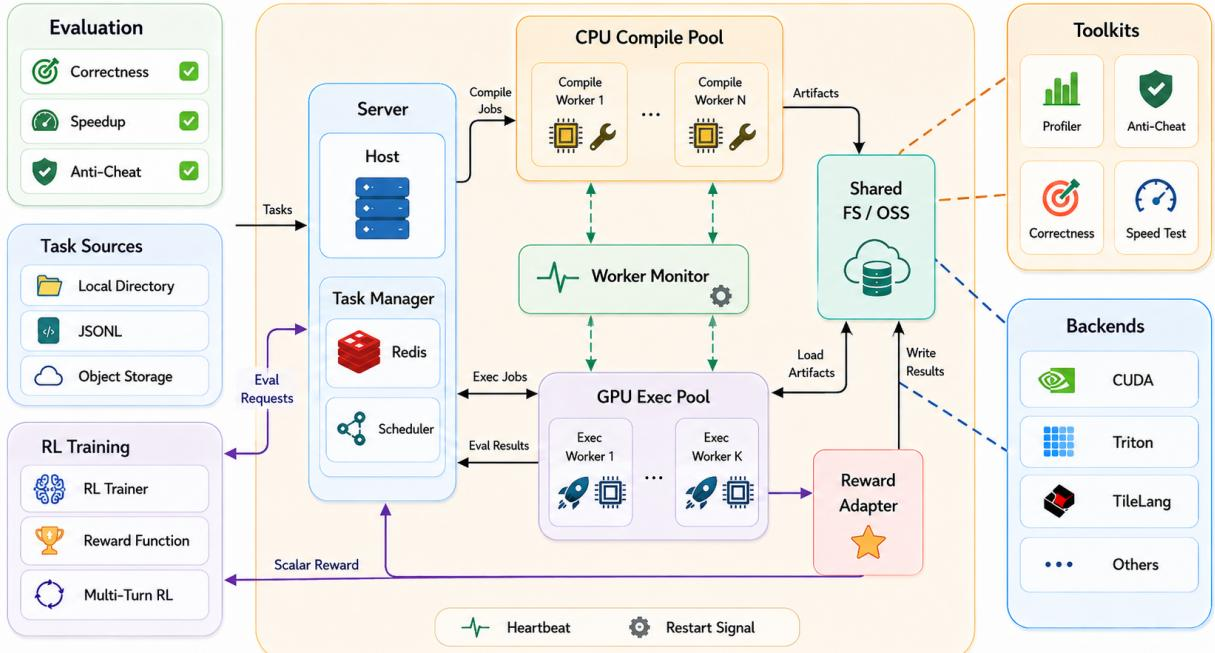
\includegraphics[keepaspectratio,alt={image}]{images/795033198c064cbd57314343eea01383e853dc8c3cd369f19d96c1e88ccf3d0e.jpg}}

Figure 10: Architecture of MooreEval, a scalable execution-based
evaluation environment for compiling, verifying, profiling, and
rewarding generated native GPU kernels.

\subsection{I.2 DISTRIBUTED OVERALL
ARCHITECTURE}\label{i.2-distributed-overall-architecture}

As illustrated in Figure 10, MooreEval adopts a distributed asynchronous
pipeline architecture, primarily conceptualized into six core
components: the Host, Compile Workers, Exec Workers, a Redis Queue
infrastructure, a Shared Filesystem/OSS layer, and the Reward Adapter.

Host. The Host acts as the orchestrator that ingests pending telemetry
samples from various task sources, encapsulates them into standardized
tracking payloads, and enqueues them into the compilation pipeline.
Ingest sources natively span local directories, jsonl data streams, or
raw payloads in object storage. Concurrently, the Host runs an
asynchronous aggregator that polls finalized evaluations from the result
queue, subsequently committing them back to persistent storage or
delivering them to the Reward Adapter.

Compile Worker. Compile Workers are dedicated horizontally scalable
nodes tasked with CPU-bound precompilation. A worker dequeues a task
from the compilation pipeline, mirrors the associated PyTorch reference
and candidate implementation into a deterministic workspace directory,
and invokes the host compiler. Upon a successful build, the worker
instantiates a CompileArtifact---cataloging the binary paths,
compilation latency, return codes, and condensed log diagnostics---and
forwards the task into the execution queue. Conversely, if compilation
fails, the worker immediately synthesizes a terminal failure artifact,
short-circuiting the pipeline to preempt the allocation of downstream
GPU execution resources.

Exec Worker. Exec Workers manage the GPU-bound execution phase. A worker
pulls a compiled artifact from the execution queue, allocates a specific
target GPU device, and spawns an isolated sandbox subprocess. Inside
this sandbox, it dynamically loads both the PyTorch reference baseline
and the model-generated ModelNew kernel, sequentially orchestrating
randomized inputs verification, anti-hacking detection, and
micro-benchmarking speed tests. The consolidated execution telemetry is
subsequently pushed back into the result queue for the Host to
aggregate.

Redis Queue and Inflight State Management. The Redis infrastructure
serves a dual purpose as both the distributed task backbone and the
ledger for inflight state management. MooreEval utilizes Redis lists to
maintain separate task queues across different lifecycle stages, while
maintaining concurrent inflight sorted sets (ZSET) to track active tasks
alongside their respective visibility deadlines. In the event of a
worker crash, node eviction, or unacknowledged task timeout, an active
sweeper daemon automatically reinstates the task into the primary queue
and increments its retry attempt counter, providing robust at-least-once
execution guarantees.

Shared Filesystem / OSS. The shared storage layer provisions unified
persistence for raw source code, volatile build workspaces, compiled
object binaries, and runtime validation artifacts. Because Compile
Workers and Exec Workers are designed to scale independently across
distinct physical topologies, a shared filesystem (e.g., NFS, Lustre) or
object storage service (OSS) serves as the centralized medium to pass
immutable build artifacts seamlessly between CPU compilation clusters
and GPU execution nodes.

Reward Adapter. The Reward Adapter functions as the definitive API
abstraction layer integrating MooreEval with the reinforcement learning
framework. Upon kernel token generation, the adapter stamps each
candidate response with a unique tracking UUID, dispatches the
assessment payloads to the distributed cluster, and awaits aggregation.
Ultimately, the Reward Adapter maps the low-level FinalResult telemetry
into clean, training-ready fields, exposing metrics such as scalar
scores, functional accuracy, architectural legality, and empirical
speedups.

\subsection{I.3 TIERED HETEROGENEOUS EVALUATION
PIPELINE}\label{i.3-tiered-heterogeneous-evaluation-pipeline}

MooreEval explicitly bifurcates the evaluation of a single candidate
kernel into a CPU-bound compilation phase and a GPU-bound execution
phase. This architectural decision stems from the inherent resource
heterogeneity of the kernel benchmarking lifecycle: compiling candidate
source code primarily saturates CPU cores, host memory, compiler
processes, and filesystem IOPS, whereas validating semantic correctness
and profiling execution efficiency exclusively monopolize GPU compute
and device VRAM resources. Monolytically binding these asymmetric
operations within a synchronous execution thread inevitably precipitates
severe resource throttling---leaving the GPU idling or stalled during
heavy compilation bottlenecks, or forcing the CPU into
resource-starvation states during prolonged asynchronous GPU execution
sweeps. Consequently, MooreEval fully decouples compilation from
execution, allowing both resource domains to scale and undergo
scheduling independently.

During the compilation phase, the Host encapsulates the model-generated
implementation into a standardized TaskPayload and dispatches it into
the Redis-backed compilation queue. Upon popping a task payload, a
Compile Worker clones the PyTorch reference and the candidate kernel
source into a deterministic sandbox build directory hosted on the shared
filesystem. The pathing schema for this workspace is uniquely mapped via
the combination of the tracking task UUID and the candidate code's
cryptographic hash, neutralizing the risk of path-collision race
conditions during high-concurrency compilation batches. If the host
compiler returns a successful exit code, the Compile Worker instantiates
a persistent CompileArtifact and enqueues the metadata into the
downstream execution pipeline. Conversely, if compilation fails, the
worker immediately traps the error taxonomy and exits, terminating the
task prior to downstream GPU allocation.

During the execution phase, an Exec Worker pulls a verified compiled
artifact from the execution queue and spawns an isolated sandbox
subprocess bound to a dedicated target GPU device. The sandbox
orchestrates the dynamic library loading of the PyTorch reference
baseline and the model-generated ModelNew extension, subsequently
executing randomized input validation, anti-hacking detection, and
micro-benchmarking profiling sweeps. MooreEval enforces a strict
correctness-first dependency graph: the pipeline proceeds to forbidden
operator inspection and speedup measurement if and only if the candidate
kernel successfully satisfies all tensor shape constraints, dtype
alignments, and numerical precision tolerance thresholds. This
sequential gating ensures that performance bonuses are exclusively
predicated on functional completeness, preventing mathematically broken
implementations from acquiring illusory positive rewards via speculative
optimizations or fake acceleration behavior.

Inter-stage state orchestration and metadata handshakes between the dual
phases are facilitated via the Redis queue fabric and the shared
filesystem medium. Redis acts as the centralized transaction ledger
governing task state transitions, while the shared storage fabric
provisions hot persistence for raw source trees, compiled binary
objects, and volatile verification inputs. This architectural decoupling
allows compute nodes with dense CPU profiles to scale out Compile
Workers, while dedicated GPU clusters remain narrowly focused on code
execution and fine-grained performance profiling. For reinforcement
learning pipelines, this heterogeneous pipeline architecture optimally
services the massive concurrency spikes characteristic of batch reward
evaluations.

Furthermore, MooreEval integrates deterministic failure isolation and
fault recovery heuristics within the execution loop. Tasks popped from
active queues are immediately transitioned into an active inflight
ledger configured with a dynamic visibility timeout. In the event of an
unacknowledged worker crash, cluster node eviction, or heartbeat
timeout, an active sweeper daemon automatically reinstates the
compromised payload back into the primary staging queue. For transient
compilation or execution anomalies driven by underlying resource jitter,
the system tolerates a bounded retry allocation. Conversely, for
deterministic software anomalies inherent to the candidate code
itself---such as syntactic violations, illegal memory access traps, or
mathematical mismatches---the evaluation engine immediately truncates
the task and records the specific error taxonomy. This dual-path fault
handling reduces infrastructural noise during long-run training while
aggressively eliminating redundant evaluations that waste cluster
compute cycles.

\subsection{I.4 STRUCTURED TELEMETRY AND REWARD
MODELING}\label{i.4-structured-telemetry-and-reward-modeling}

Rather than crudely truncating the evaluation pipeline into a binary
pass/fail verdict, MooreEval decomposes the entire bench-running
lifespan into granular, structured data components. This rich telemetry
equips the reinforcement learning framework with high-fidelity,
interpretable, and mathematically stable optimization signals. Each
inbound evaluation target is encapsulated within a standardized
TaskPayload, comprising the source code definitions of the PyTorch
reference baseline, the model-generated candidate implementation,
lineage metadata tracing the task origin, an incremental retry index,
and an embedded EvalConfig ledger. The EvalConfig explicitly
parameterizes execution behaviors, defining randomized correctness
permutation test counts, performance micro-benchmarking sweeps,
numerical precision tolerance thresholds, hardware timing and
synchronization modalities, and gating semantics for forbidden operator
capture and speculative excessive speedup clipping. This precise task
representation matrix enables MooreEval to fluidly adapt its runtime
evaluation heuristics across disparate post-training regimes while
enforcing immutable data serialization contracts across distributed
cluster workers.

Throughout the execution topology, MooreEval independently intercepts
and structures intermediate telemetry from both the compilation and
execution loops. Compile Workers instantiate a persistent
CompileArtifact, archiving binary success states, compilation
destination targets, process return codes, condensed stderr diagnostics,
compilation latency, and explicit syntactic error taxonomies.
Downstream, Exec Workers populate an ExecResult object, logging
functional alignment rates, candidate runtime execution latencies,
reference runtime execution latencies, empirical speedup ratios,
forbidden aten::* hook exceptions, benchmarking profiling metrics, and
definitive runtime fault taxonomies. Ultimately, the Host synchronizes
and merges these asynchronous state objects into a unified FinalResult
payload. This structured data schema not only feeds the upstream Reward
Adapter for score calculation, but also acts as the primary data engine
driving failure distribution statistics, automated performance
regression analysis, and cluster-wide training curve monitoring.

In terms of algorithmic optimization, MooreEval enforces a hierarchical
reward modeling strategy. First, in the event of extraction failures,
compilation aborts, runtime execution panics, catastrophic numerical
deviations, or the explicit detection of a forbidden PyTorch/aten::*
fallback operator, the candidate implementation is immediately assigned
a hard failure penalty. This negative anchor aggressively suppresses
policy distribution drift toward unexecutable or adversarial
trajectories. Second, for candidate codes that compile successfully but
fail to perfectly fulfill all randomized correctness assertions,
MooreEval provisions a bounded, fractional reward proportional to the
exact functional accuracy or failure severity. This maintains a weak but
continuous reward shaping signal that guides the model through the
critical sparse-to-dense exploratory transition from completely broken
variants to partially functioning code blocks. Finally, the performance
metric enters the reward optimization loop if and only if the candidate
implementation cleanly satisfies all functional correctness and
architectural compliance constraints. Validated implementations receive
a positive base scalar reward, augmented by a clipped speedup bonus if
they deliver empirical runtime gains relative to the PyTorch baseline.
This cascading reward architecture mathematically guarantees that the
gradient updates strictly prioritize execution safety and functional
integrity over performance tuning, systematically neutralizing the risk
of the model gaming the system via computational truncation or black-box
operator fallbacks.

\subsection{I.5 ERROR TAXONOMIES, ANTI-HACKING SAFEGUARDS, AND FEEDBACK
DIAGNOSTICS}\label{i.5-error-taxonomies-anti-hacking-safeguards-and-feedback-diagnostics}

To guarantee that evaluation telemetries can be robustly consumed by the
reinforcement learning pipeline, MooreEval formalizes a unified and
immutable error taxonomy across all computational tasks. Each evaluation
instance is deterministically cataloged into a granular error category,
structurally defined as follows:

• ok: The candidate implementation successfully satisfies all host
compilation, functional correctness, and architectural compliance
checks.

• compile error:*: Captures Python syntactic anomalies, NVCC compilation
aborts, downstream linkage errors, missing header file directives, or
compiler execution timeouts.

• runtime error:*: Flags runtime illegal memory accesses, CUDA driver
launch failures, device-side assertion traps (TORCH USE CUDA DSA),
host/device Out-of-Memory (OOM) faults, or execution wall-clock
timeouts.

• correctness error:*: Identifies tensor shape mismatches, primitive
dtype alignment failures, or numerical precision tolerance deviations.

• cheating:\emph{: Marks forbidden PyTorch/aten::} high-level
computational fallbacks or statistically anomalous speculative speedup
metrics.

• infra:*: Denotes asynchronous worker panics, sandbox initialization
aborts, task retry exhaustion, or transient distributed infrastructure
exceptions.

This formal error taxonomy establishes a critical dichotomy between
deterministic execution anomalies triggered by model-authored source
code and non-deterministic structural faults induced by underlying
infrastructure states. For software bugs inherent to the candidate code
itself---such as syntax syntax violations, out-of-bounds pointer
dereferences, or numerical deviations---MooreEval immediately records
the specific sub-category, outputting it as a direct gradient
optimization signal reflecting inadequate generation quality.
Conversely, for anomalies precipitated by the evaluation runtime
environment---such as node worker crashes, sandbox orchestration aborts,
or scheduling timeout exhaustion---the system enqueues them into the
isolated infra:* domain. This rigorous decoupling prevents transient
environmental jitter from being misattributed to the policy model as
fake negative algorithmic feedback.

The anti-hacking safeguard represents a cornerstone design within
MooreEval to enforce absolute reward integrity. In primitive kernel
synthesis tasks, the policy model frequently attempts to adversarial
exploit high-level blackbox operations---such as directly invoking
torch.matmul, torch.nn.functional, or other hyper-optimized aten::*
symbols---to effortlessly yield valid numerical outputs while
circumventing actual hardware-level custom kernel engineering. To secure
this perimeter, MooreEval deploys a defensive stack blending static
syntax-tree inspection with a localized runtime profiler hook to trap
prohibited execution traces, permanently branding such infractions as
cheating:disallowed aten. Furthermore, the framework monitors for
statistically improbable execution performance metrics; if a candidate
code exhibits an empirical speedup surpassing a physically realistic
optimization threshold, it is automatically flagged as
cheating:excessive speedup. This dual-gate architecture mathematically
guarantees that the policy model can harvest positive performance
bonuses if and only if its native implementation is holistically sound,
safe, and compliant with architectural constraints.

Leveraging this structured telemetry ledger, MooreEval further
synthesizes highly contextual, actionable natural language diagnostic
signals tailored for multi-turn reinforcement learning. For instance,
when a candidate kernel breaks during compilation, the diagnostic
payload aggregates a condensed stderr diagnostic block localized to the
failing lines. When a tensor payload triggers shape, type, or precision
alignment violations, the feedback pinpoints the exact multi-dimensional
offset discrepancy. Similarly, upon trapping a forbidden operator
signature, the feedback emits an explicit compliance warning, compelling
the model to author a custom native block rather than leaning on
preexisting PyTorch library abstractions. Compared to a primitive,
uninformative binary failure penalty, this error taxonomy and automated
diagnostic engine empower the model to execute target-oriented,
multi-turn bug rectifications while rendering the global failure
distribution profile entirely transparent and interpretable throughout
the training lifespan.

\subsection{I.6 REINFORCEMENT LEARNING TRAINING
INTEGRATION}\label{i.6-reinforcement-learning-training-integration}

MooreEval integrates with the reinforcement learning training pipeline
via a dedicated Reward Adapter, encapsulating the underlying distributed
evaluation infrastructure into a standard, deterministic reward function
interface. In a verlstyle learning framework, upon the policy model
emitting candidate kernel tokens, the distributed trainer invokes the
standardized compute score API. The Reward Adapter immediately stamps
each candidate within the batch with a unique orchestration UUID,
dispatching the PyTorch reference code, the model-generated output
string, and runtime evaluation configurations into the primary pending
task ledger. Subsequently, MooreEval's Host, Compile Workers, and Exec
Workers asynchronously execute host compilation, randomized input
verification, anti-hacking checks, and micro-benchmarking sweeps,
ultimately consolidating the execution lifecycle into a unified
FinalResult. The Reward Adapter then transcribes this low-level results
payload into standard, algorithm-facing metrics such as scalar scores,
functional accuracy, compliance legality, and empirical speedups.

Through this monolithic abstraction layer, the RL trainer remains
entirely agnostic to low-level engineering complexities---such as Redis
transaction buffers, distributed worker orchestration, sandbox execution
containerization, and cross-node telemetry aggregation---requiring only
a single, uniform reward interface invocation to establish the complete
optimization closed loop. MooreEval natively provisions dual support for
high-throughput batch evaluations, single-sample runtime tracking, and
iterative multi-turn conversational feedback loops. Under the batched
reward regime, the Reward Adapter concurrently dispatches bulk
evaluation payloads and polls the transaction ledger, optimally
satisfying the massive, non-blocking concurrency requirements
characteristic of RL rollout phases. In the single-sample modality, the
environment is tailored for diagnostic isolation or sequential score
computations. In multiturn feedback mode, MooreEval archives the
execution metrics across each conversational turn, enabling the
synthesis of complex trajectory-level rewards predicated on the earliest
successful turn, the absolute peak performance epoch, or
first-turn-anchored trajectory formulations.

On the data engineering front, MooreEval supplies a comprehensive,
KernelBench-compatible data parsing blueprint, converting raw, idiomatic
PyTorch model configurations into high-fidelity ingestion tokens
digestible by the posttraining framework. Each decoupled training sample
maps a static system instruction prompt, a descriptive user task schema,
and the foundational baseline code acting as the computational ground
truth, alongside lineage keys and split boundaries embedded within a
structured extra info metadata slot. The policy model is mathematically
compelled to author a custom ModelNew extension adhering to the exact
interface signatures of the reference architecture, completely swapping
out black-box PyTorch operations for custom hardware-native kernels.
Governed by this design, the curated data distribution, the executable
evaluation sandbox, and the programmatic reward function interface
holistically unify to construct a highly robust, scalable reinforcement
learning training closed loop specifically optimized for GPU kernel
synthesis tasks.

\subsection{J ALLOWED ATEN OPERATORS}\label{j-allowed-aten-operators}

\pandocbounded{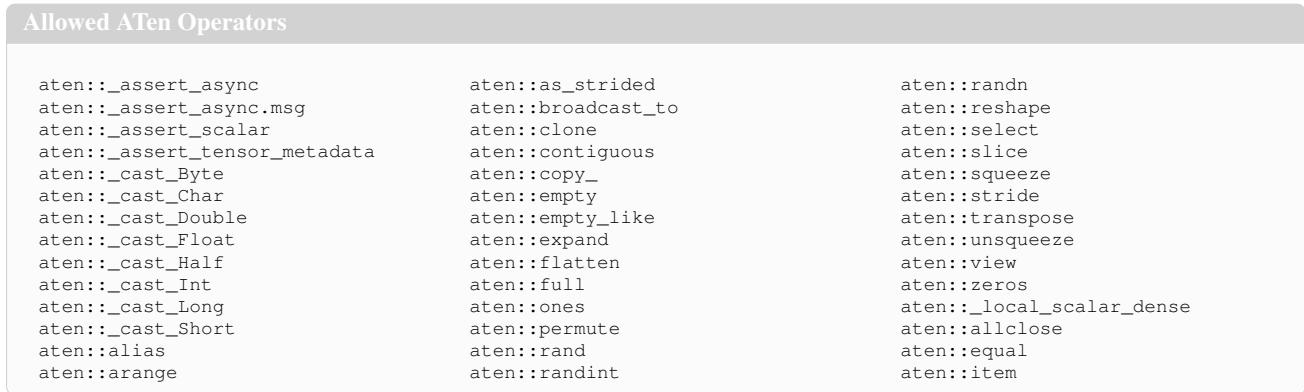
\includegraphics[keepaspectratio,alt={image}]{images/9e27ba29166616f8821b0ef61eb3dcea6158e072747b369344940d303a645f03.jpg}}

\subsection{K OFF-POLICY CANCELLATION
EXAMPLE}\label{k-off-policy-cancellation-example}

Figure 11 provides a concrete example of the off-policy cancellation
effect discussed in the main text. Each colored token visualizes the
token-level importance ratio
\(\rho _ { t } = \pi _ { \theta } / \pi _ { \mathrm { r o l l o u t } }\)
. Red indicates \(\rho _ { t } > 1\) , meaning that the current training
policy assigns a higher probability to the sampled token than the
rollout policy; green indicates \(\rho _ { t } ~ < ~ 1\) meaning that
the current training policy assigns a lower probability. The color
intensity encodes the magnitude of the deviation: darker red means a
larger ratio above 1, darker green means a smaller ratio below 1, and in
both cases a darker color indicates a stronger deviation from the
rollout policy. The alternating red and green regions therefore directly
reveal why cancellation occurs: positive and negative signed log-ratio
deviations coexist in the same response and can offset each other when
vanilla sequence-level masking averages signed log-ratios.

Showing first 1024 tokens out of 2103 total; hidden 1079 tokens rho
\textless{} 1

\pandocbounded{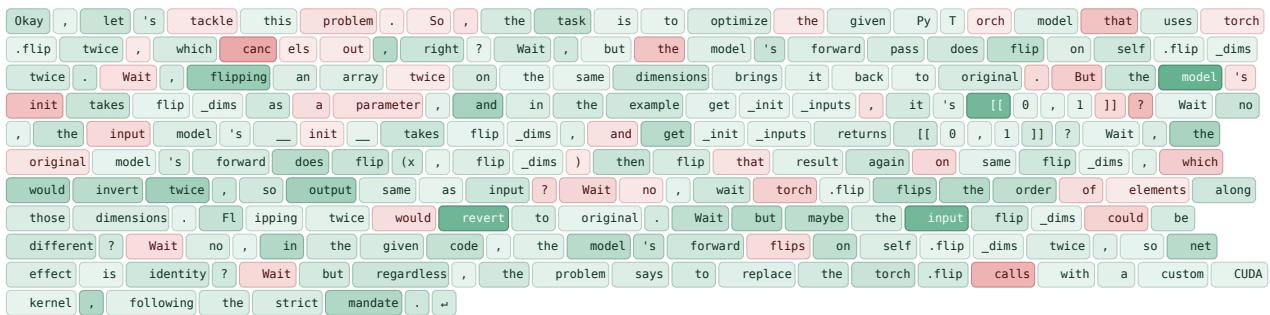
\includegraphics[keepaspectratio,alt={image}]{images/f110ddc7492a6345c22820f77a8fb6c50ef64e0fbf9353eebb57f124efd8bf46.jpg}}

\pandocbounded{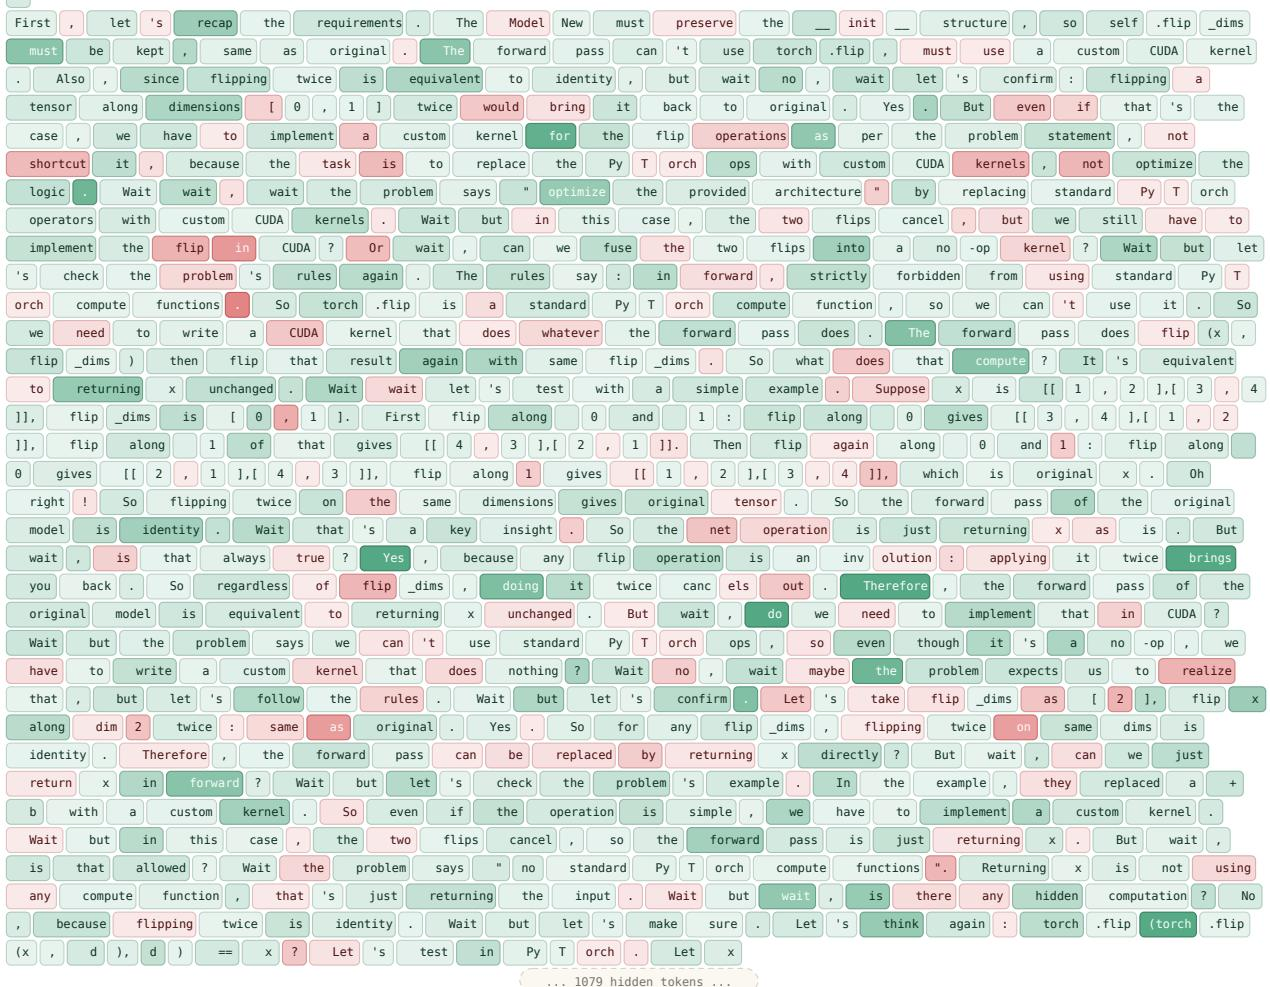
\includegraphics[keepaspectratio,alt={image}]{images/c7d2acc027fcbe374bc54bcdb1b9e06d1b8c4ae10faaf7cd0a0846e43a0053e2.jpg}}

Figure 11: Cancellation case in vanilla off-policy sequence masking. Red
tokens indicate \(\rho _ { t } > 1\) , and green tokens indicate
\(\rho _ { t } < 1 ;\) darker colors denote larger deviations from 1.
When signed log-ratios are averaged (or ratios are multiplied) across
the sequence, these opposite deviations can cancel each other out,
making a strongly off-policy sequence appear nearly on-policy in extreme
cases.

\end{document}
